\documentclass{ucdgradtaughtthesis}
\usepackage{multirow}
\usepackage{pdfpages}
%%\PassOptionsToPackage{a4paper,left=30mm,top=20mm,right=20mm,bottom=30mm}{geometry}
%\usepackage[backend=biber,style=numeric]{biblatex} % Use biblatex with numeric citations
\usepackage{geometry}  % Use the geometry package
\geometry{
    a4paper,            % Paper size
    left=30mm,          % Left margin
    right=20mm,         % Right margin
    top=20mm,           % Top margin
    bottom=30mm,     % Bottom margin
}
\usepackage{cite}
\usepackage{hyperref}  
\usepackage{tikz}
\usetikzlibrary{positioning}
\usepackage{subcaption}
\usepackage{ulem} 
\usepackage{comment}
\usepackage{amsmath}
\usepackage{float} 
\setlength{\parskip}{0.5em}
% Enable clickable references    
\usepackage{array}
\usepackage{graphicx}    
\usepackage{adjustbox}
\usepackage{makecell}
\usepackage{csvsimple}
\usepackage{fancyhdr}
\pagestyle{fancy}
\usepackage{amssymb}
\usepackage{setspace}

\onehalfspacing
\newcommand{\Sarp}[1]{{\textcolor{blue}{{SA: #1}} }}
\newcommand{\Sean}[1]{{\textcolor{red}{{Sean: #1}} }}
\newcommand{\todo}[1]{\textcolor{orange}{\texttt{TODO: #1}}}


\lhead{\fancyplain{}{\textbf{\large\leftmark}}}
\rhead{\fancyplain{}{\textbf{\large\rightmark}}}
\setlength{\headheight}{30pt}
\renewcommand{\chaptermark}[1]{\markboth{\chaptername\ \thechapter. #1}{}}
\renewcommand{\sectionmark}[1]{\markboth{}{\thesection.#1}}


\bibliographystyle{plainurl}

 % without .bib extension



 \title{Guassian Process Regression for Gravitational Waves}
 \author{Seán White}
 
 \degree{BSc Applied and Computational Mathematics}
 
 \college{Science}
 \school{School of Mathematics and Statistics}
 
 \supervisor{Dr. Sarp Ak\c{c}ay}
 
 \thesisdate{\today}



\begin{document}
\pagestyle{plain}


\maketitle

\begin{abstract}
    The gold standard Gravitational Waveforms (GWS) for merging black holes are generated by Numerical relativity (NR) simulations, but they are computationally expensive. 
    Analytic approximations reduce this cost yet introduce errors when compared with NR results. A recent method (NR informed method) has been developed to use these errors (quantified by the waveform mismatch) in a bayesian framework to select the most accurate model in each region of the parameter space.
    However, computing mismatches across vast parameter domains still requires many NR simulations. To mitigate this cost, we propose a Gaussian Process Regression (GPR) model to predict mismatches efficiently.

    We begin by reviewing Gaussian Process fundamentals and systematically test various kernels (RBF, Matern, Rational Quadratic, Laplacian) under both homoscedastic and heteroscedastic noise. 
    Cross-validation on six performance metrics narrows the field to eight finalist models, which we then retrain on 90\% of the data and evaluate on a 10\% holdout. 
    Models assuming constant (homoscedastic) noise prove too simplistic, while those relying on known noise values struggle in regions with sparse data. 
    Our best-performing model ( a heteroscedastic GPR with an additive RBF-Matern kernel) achieves an \(R^2 \approx 0.99\) and an RMSE of \(\sim 0.034\), demonstrating robust predictive accuracy.

    To capture uncertainty in the kernel hyperparameters, we build a posterior distribution over the hyper-parameters using Markov Chain Monte Carlo (MCMC) simulations. 
    We compare the resulting marginal predictive distribution with pointwise predictions and, for computational practicality, adopt the pointwise model as our final choice. 
    This GPR-based model offers a computationally efficient alternative for estimating waveform mismatches, reducing reliance on costly NR simulations across the parameter space. 
    Our GPR model therefore enables more efficent use of the NR-informed method in GW parameter estimation.
\end{abstract}
    

\chapter*{Acknowledgments}
I would like to thank .....

\tableofcontents
\listoffigures
\listoftables

% Normal Chapters. Switch to arabic numbers and turn headers on
\clearpage
\pagenumbering{arabic}
\pagestyle{fancy}


\chapter{A brief Introduction to Gravitational Waves}
\section{Plane Wave Solution from General Relativity}
\label{sec:GRintro}
\todo{Consistent I/we}
Gravitational waves (GWs) are small fluctuations of spacetime that propagate at the speed of light. In the simplified linearized theory, we assume a flat (Minkowski) geometry for the background spacetime, and the small fluctuations about it satisfy the wave equation in an appropriate gauge (specific choices of coordinates). This is described in detail in Gravitational Waves, Vol. 1 by Maggiore~\cite[Sec~ 1.1]{GRbook}, we provide brief
details here.

Formally we start by perturbing the flat Minkowski metric $\eta _{a b}$ by a small amount encoded by
the metric perturbation $h_{a   b}$
\begin{equation}
g_{ab} = \eta_{ab} + \epsilon\,h_{ab},
\qquad
\epsilon \ll 1,
\qquad
\eta_{ab} = \mathrm{diag}(-1, 1, 1, 1).
\end{equation}
This is then substituted into the Einstein field equation whereby only terms linear in $h_{ab}$ are kept,
the so-called linearized regime of general relativity. 
Using the trace-reversed variable $\bar{h}_{ab}:= h_{ab}-\tfrac{1}{2} \eta_{ab} h_c^{\ c}$,
the Einstein field equation simplifies to
\begin{equation}
    \Box \bar{h}_{ab} = \frac{-16\pi G}{c^4} T_{ab}.
\end{equation}
However we are interested in this equation outside of the source (i.e $T_{ab} =0$), therefore we are left with 
\begin{equation}
    \Box \bar{h}_{ab} = 0, 
\end{equation}
with \(\Box\) the d’Alembertian operator in flat spacetime.
%

Although \(h_{ab}\) initially has 10 independent components (as a symmetric $4 \times 4$ rank-2 tensor), 8 of these correspond to gauge freedom and constraints. After imposing the Lorenz and transverse-traceless (TT) gauge conditions, only two physical degrees of freedom remain: the plus (\(h_+\)) and cross (\(h_\times\)) polarizations~\cite[Sec.~1.2]{GRbook}.
This wave equation admits plane-wave solutions. For a wave propagating in the \(z\)-direction, the TT-gauge form of the perturbation is
\begin{equation}
h_{ab}^{(\mathrm{TT})} \;\propto\;
\begin{pmatrix}
0 & 0 & 0 & 0 \\
0 & h_+ & h_\times & 0 \\
0 & h_\times & -h_+ & 0 \\
0 & 0 & 0 & 0
\end{pmatrix}
e^{i(kz-\omega t)}.
\end{equation}


\subsection{Leading-Order Power Emission by Gravitational Waves}
\label{subsec:GW_power}
In general, the power emitted by a radiative field can be expressed schematically as
\begin{equation}
    \dot{E} = \sum_{\ell = 0}^{\infty} \left\langle \left| \left( \frac{\partial}{\partial t} \right)^{\ell+1} P_\ell(t) \right| \right\rangle.
\end{equation}
Here, \(P_{\ell}(t)\) represents the multipole moments of the radiating source. The \(\ell = 0\) term corresponds to the monopole moment, which in the gravitational case is the total mass of the system. Assuming mass is conserved, this term vanishes.
The \(\ell = 1\) term represents the dipole moment, which is also zero in the gravitational case due to conservation of linear momentum. Therefore, the leading-order contribution to gravitational-wave emission arises from the \(\ell = 2\) term, known as the quadrupole radiation.
This gives the leading-order expression for the power emitted in gravitational waves
%
\begin{equation}
\dot{E} = \frac{G}{5\,c^5}
\left\langle \dddot{Q}_{ij}\,\dddot{Q}^{\,ij} \right\rangle,
\end{equation}
%
where \(Q_{ij}\) is the mass quadrupole moment of the source. It is related to the mass moment \(M_{ij}\) by
%
\begin{equation}
Q_{ij} := M_{ij} - \frac{1}{3} \delta_{ij} M^k_{\ k},
\end{equation}
where \(M_{ij} = \int d^3x\, T^{00}x^i x^j\).



\subsection{Quasi-circular Inspiral of two Point Masses}
\label{subsec:two_mass_example}
We will now consider a generic problem as illistrated in \cite{intoGRSarp} where two point masses, \(m_1 \ge m_2\), are in a quasi-circular orbit of separation \(R\),
each at distances \(r_1\) and \(r_2\) from their common center of mass (CoM), with
\(R = r_1 + r_2\). We place the orbit in the \(x\)--\(y\) plane so that mass~1 moves on
\(\mathbf{x}_1(t) = r_1(\cos\Omega t,\,\sin\Omega t)\) and mass~2 on
\(\mathbf{x}_2(t) = r_2(\cos(\Omega t+\pi),\,\sin(\Omega t+\pi))\). The system’s orbital
frequency is \(\Omega\). A short calculation yields
%
\begin{equation}
    Q^{ij} = 4 \Omega^3 \left(m_1 r_1^2 + m_2 r_2^2\right)
    \begin{pmatrix}
    \sin(2\Omega t) & -\cos(2\Omega t) \\
    -\cos(2\Omega t) & -\sin(2\Omega t)
    \end{pmatrix}.
\end{equation}
%
%
Introducing the reduced mass \(\mu = m_1 m_2/(m_1 + m_2)\), we get that the \(\ell=2\) power emission is
%
\begin{equation}\label{eq:E_dot_2}
\dot{E}_{\ell=2}
\;=\;
\frac{32}{5}\;\frac{G}{c^5}\;\Omega^6\,\mu^2\,R^4.
\end{equation}
Here \(G\) is Newton's gravitational constant and c is the speed of light. Both \(\Omega\) and \(R\) are functions of time, but they evolve on a time scale (radiation reaction) much longer than the orbital time
scale and so when averaging over orbits we approximate them as constant. Applying Kepler’s law, \(\Omega^2 = GM/R^3\), and defining
\(\omega = 2\Omega\) as the GW frequency, we find
%
%
\begin{equation}
\dot{E}_{\ell=2}
\;=\;
\frac{32}{5}\;\frac{c^5}{G}
\left(\frac{G\, M_c \;\omega}{2c^3}\right)^{10/3},
\quad
\text{where}
\quad
M_c \;=\;\mu^{3/5}\,M_{\text{tot}}^{2/5}
\label{eq:Energy}
\end{equation}
%
is known as the chirp mass where $M_{\text{tot}} = m_1+m_2$ is the total mass.
%
%
$ \dot{E} $ represents the rate at which the system loses energy due to gravitational-wave emission.
This energy loss causes the binary orbit to shrink and the GW frequency to increase, 
with the chirp mass \(M_c\) and frequency \(\omega\) capturing the key features of this inspiral.
%

In general, an incoming GW manifests itself as a time series of GW strain given by
\begin{equation}
 h(t) = h_+(t) - i h_\times(t), \label{eq:GW_strain}
\end{equation}
%
where $ h_+, h_\times$ are the two physical degrees of the GW known as the polarizations.
For the case of the simple quasi-circular inspiral introduced above, 
the polarizations can be expressed in terms of the characteristic strain \( h_c(t) \) [Sec~\cite[Sec.~4.1]{GRbook}]
which captures the amplitude of the waveform
\begin{subequations}
\begin{align}
h_+(t) &= h_c(t) \left( \frac{1 + \cos^2\iota}{2} \right) \cos[\Phi_N(t)],
\label{eq:hp_time}\\
h_\times(t) &= h_c(t) \cos\iota \sin[\Phi_N(t)],
\label{eq:hc_time}\\
h_c(t) &= \frac{4}{D} \left( \frac{G M_c}{c^2} \right)^{5/3} \left( \pi f(t) \right)^{2/3}
\label{eq:char_strain}.
\end{align}
\end{subequations}
Here \(\iota = \cos^{-1}(\hat{n} \cdot \hat{L}) \) is the inclination angle between the line-of-sight unit vector \( \hat{n} \) and the orbital angular momentum unit vector \( \hat{L} \),
\( M_c \) is the chirp mass,
\( D \) is the distance to the source and \(f(t)\) is the GW frequency, defined by \(\frac{\omega (t)}{2\pi}\).
As the frequency \( f(t) \) increases, so too does \( h_c(t) \), giving rise to the characteristic chirping waveform.
%

To compare these theoretical waveforms with NR simulations it is necessary to have the
Fourier transform of the GW amplitudes. The resulting forier transforms of Eqs.~(\ref{eq:hp_time}, \ref{eq:hc_time})
are stated below and derived in Sec~\cite[Sec.~4.1]{GRbook} :
\begin{subequations}
    \label{eq:hfreq}
    \begin{align}
        \tilde{h}_+(f) &= A e^{i \Psi_+(f)} \frac{c}{D} \left( \frac{G M_c}{c^3} \right)^{5/6} \frac{1}{f^{7/6}} \left( \frac{1 + \cos^2 \iota}{2} \right), \label{eq:hplus_freq} \\
        \tilde{h}_\times(f) &= A e^{i \Psi_\times(f)} \frac{c}{D} \left( \frac{G M_c}{c^3} \right)^{5/6} \frac{1}{f^{7/6}} \cos \iota, \label{eq:hcross_freq}
    \end{align}
\end{subequations}
%
%
where the constant \( A \) and the phases are given by
\begin{subequations}
    \begin{align}
        A &= \frac{1}{\pi^{2/3}} \left( \frac{5}{24} \right)^{1/2}, \label{eq:A_amp} \\
        \Psi_\times(f) &= \Psi_+(f) + \frac{\pi}{2}, \label{eq:psi_cross} \\
        \Psi_+(f) &= 2\pi f \left( t_0 + \frac{D}{c} \right) - \Phi_0 - \frac{\pi}{4} + \frac{3}{4} \left( \frac{G M_c}{c^3} 8\pi f \right)^{-5/3}. \label{eq:psi_plus}
    \end{align}
\end{subequations}
%
Here \( t_0 \) represents the constant time shift and \( \Phi_0 \) represents the constant phase shift.
%

\subsection{Introducing the Waveform Mismatch}
\label{subsec:mismatch_intro}
%
%
This simplified two-mass, circular-orbit model captures the main physical features of an inspiraling binary system, such as the characteristic chirp behaviour.
However, it omits several important physical effects, including orbital eccentricity and the spins of the individual masses. 
To quantify the impact of these simplifications on waveform accuracy, we compute the mismatch between the simplified waveform, 
\( h_i \), and more accurate (or faithful) waveforms \( h_0 \), such as those generated using numerical relativity.
The mismatch between two signals is defined in \cite{mismatch, Ogpaper} as:
%
\begin{equation}
\label{eq:mismatch_def}
\mathcal{M} = 1 - \max_{\boldsymbol{\lambda_m}}
\frac{\langle h_i,\,h_0 \rangle}{\sqrt{\langle h_i,\,h_i \rangle \,\langle h_0,\,h_0 \rangle}},
\end{equation}
%
where \( \langle \cdot, \cdot \rangle \) denotes the inner product of two waveforms in the frequency domain defined as:
%
\begin{equation}
\langle h_i,\,h_0 \rangle = 4\,\mathrm{Re} \int_{f_{\text{min}}}^{f_{\text{max}}} \frac{\tilde{h}_i^*(f)\,\tilde{h}_0(f)}{S_n(f)}\,df,
\end{equation}
%
where \( \tilde{h}(f) \) represents the Fourier transform of the gravitational waveform (Eq.~\eqref{eq:hfreq}), the asterisk denotes complex conjugation, and \( S_n(f) \) is the detector’s noise averaged over multiple noise realisations.
We finally maximise over a set of (intrinsic and/or extrinsic) model parameters \(\mathbf{\lambda_m}\) depending on the type of mismatch we wish to compute
 (see Section~\ref{sec:data_description} for details on these parameters).
A mismatch \(\mathcal{M}\ll 1\) indicates that a given waveform
faithfully represents the ``physical'' (NR) signal, whereas larger mismatches highlight missing
physics (overly simplified).




\section{GW Approximation using Bayesian Methods}
\label{sec:GW_and_Bayes}

In Section~\ref{sec:GRintro} we focused on linearised theory and a simple Newtonian two-body inspiral model. This helped motivate the ideas behind gravitational wave generation and emisson.
However the gold standard for generating gravitational waveforms is to directly solve the full Einstein equations via numerical relativity (NR),
but, the computational cost is enormous, and therefore only a limited number of NR simulations are currently available.
Consequently, many analytic or semi-analytic GW models have been created that are calibrated to these NR simulations.
As each waveform model makes a various set of differing assumptions to others models, it introduces model-specific
errors and potentially biases.
We utilise the mismatch between signals discussed in Section~\ref{subsec:mismatch_intro} 
to quantify how faithful GW waveforms generated by a given model are to the NR simulations.
%
%

The standard approach to account for modelling errors when inferring the properties of binary black holes is to construct a mixture model, where results from multiple waveform models are combined.
Bayesian methods are employed to build posterior distributions for each model over model parameters (Mass, Spin vectors, etc.) given the data. Different approaches exist for combining these posteriors:
\begin{itemize}
    \item Standard Method \cite{linearcombination}: Combine all model-specific posterior distributions with equal weights yielding a single mixture distribution.
    \item Evidence-Informed Method \cite{Bayesianapproach}: Weigh each model by its Bayesian evidence i.e., by how well it fits the observed data overall. 
\end{itemize}
%
%

These methods fail to account for the fact that some waveform models may be more faithful to full NR solutions in certain regions of parameter space (e.g., certain mass ratios or spin orientations),
while others do better in other regions. Combining all posteriors equally or by weights determined by over-all model performance does not account for these local variations in model accuracy.
To address this, Hoy et al.~\cite{Ogpaper} proposed a numerical relativity-informed strategy that uses waveform mismatch to evaluate local model accuracy across the parameter space. 
Bayesian inference is employed to favour the model with the lowest mismatch at each point in the parameter space, thereby improving the robustness of parameter estimation.
%

An illustrative example of this is shown in Figure~\ref{fig:projectmotivation}, taken from Hoy et al.~\cite{Ogpaper}. It shows a scatter plot of the posterior samples for two total spin projections generated from the parameter estimation recovery of the injection of the synthetic GW signal \textsc{SXS:BBH:0926}~\cite{NRsimulation} into LIGO noise. 
Contours over these points represent the ratio of mismatches (to NR) between different waveform models.
In the left panel, the contour plot of the ratio of \textsc{IMRPhenomTPHM}-NR \textsc{SEOBNRV5PHM}-NR mismatches is shown with the right panel showing the same for \textsc{IMRPhenomXPHM}\cite{NRfitMP}.
A mismatch ratio greater than one indicates that the \textsc{SEOBNRV5PHM}~\cite{bestNRfitS} produces waveforms that more closely match NR than the model it is being compared against.
We see that \textsc{SEOBNRV5PHM} yields mismatches that are approximately \( \sim 3\times \) and \( \sim 1.8\times \) smaller, respectively.
This relatively large difference in model performance motivates the NR informed strategy
which will favour \textsc{SEOBNRV5PHM} in these parameter regions where it is more accurate. 
Hoy et al.~\cite{Ogpaper} showed that using this technique uses 30\% less computational resources, and more faithfully recovers the true parameters than
the existing techniques.
%

\begin{figure}[H]
    \centering
    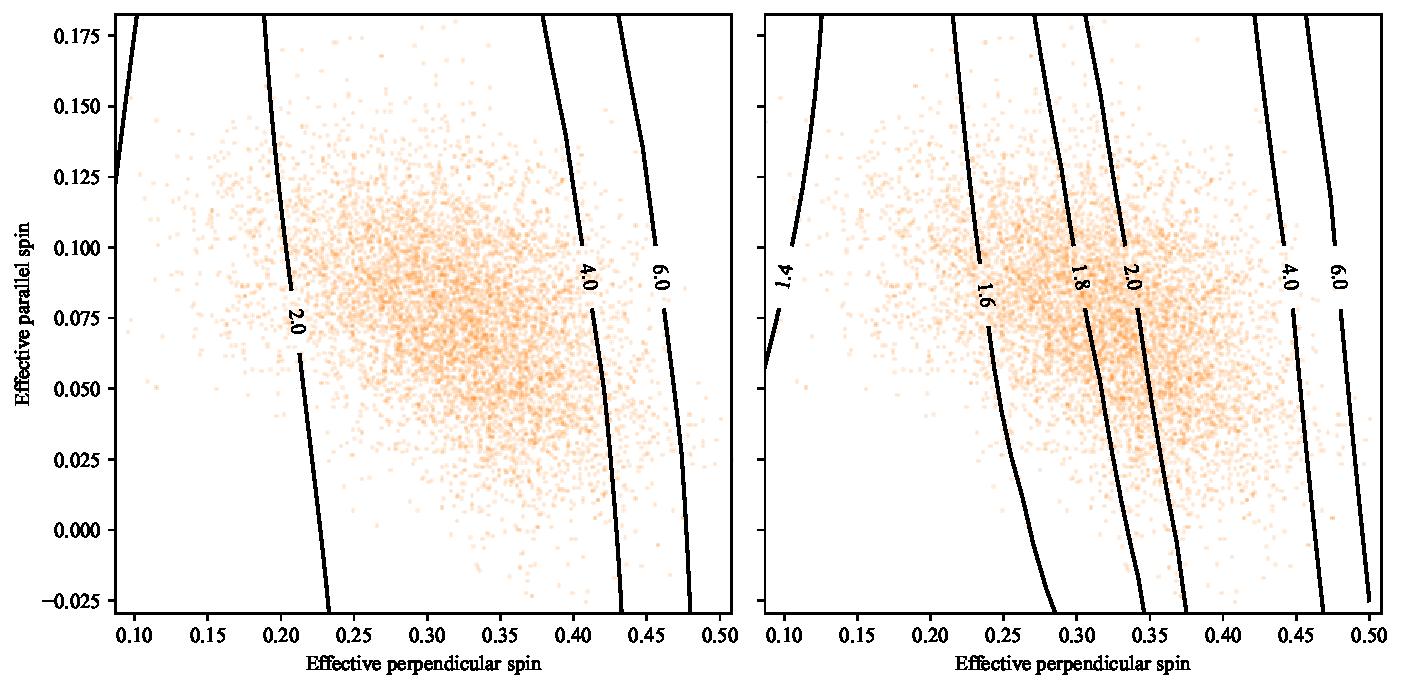
\includegraphics[width=\textwidth]{LatexPlots/HoyFigure2.pdf}
    \caption[Motivating the NR Bayesian Method.]{Contour plots showing the ratio of mismatches with respect to NR simulations, for different effective parallel and perpendicular spin components, averaged over a range of mass ratios. 
    The left plot shows \( \mathcal{M}(\textsc{IMRPhenomXPHM}) / \mathcal{M}(\textsc{SEOBNRV5PHM}) \), and the right shows \( \mathcal{M}(\textsc{IMRPhenomTPHM}) / \mathcal{M}(\textsc{SEOBNRV5PHM}) \).}
    \label{fig:projectmotivation}
\end{figure}





\section{Project Motivation}
Although the NR-informed method is conceptually appealing, it requires us to know (or at least to estimate) 
the mismatch of each model throughout the parameter space of interest. Because
NR simulations are costly, we cannot generate an exhaustive library of NR waveforms
everywhere. This is where the work summarized in this thesis comes in.
%

We propose to build a GPR model that predicts the mismatch as a function of parameters. Specifically, from a finite set of computed mismatches (obtained at a limited but carefully chosen set of parameter points), we train a GPR.
The trained model can then predict the mismatch in the untested regions of parameter space. This approach circumvents the need for high-resolution NR simulations at every point of interest,
offering an efficient and scalable alternative. The Gaussian Process framework is advantageous because it not only provides a smooth fit but also yields uncertainty estimates for its predictions.
As more NR data become available, the GPR can be updated or retrained, systematically improving the global mismatch predictions.
By modeling the mismatch between approximate waveforms and NR waveforms via GPR, we can then better implement the mismatch-driven approach introduced by Hoy et al.~\cite{Ogpaper}. 

\section{Data Description}
\label{sec:data_description}
Our proposed GPR method will take as inputs the intrinsic parameters of the binary black hole and will output the mismatch predictions.
The inrinsic parameter space of a binary black hole is eight dimensional (two masses and two spin 3-vectors) as highlighted by Figure~\ref{fig:gr_diagram}. 
To generate this mismatch data we calculated the mismatch between waveform model \textsc{SEOBNRv5PHM} \cite{bestNRfitS} and the NR surrogate \textsc{NRSur7dq4} \cite{NRsurrogate} using eqn~\eqref{eq:mismatch_def} for a set of 250 intrinsic parameters 
such that it covers 5 different mass ratios and a grid of concentric ellipses in the spin projection space.
This 250 element set is then repeated for 4 different masses.
Each mismatch is further an average of 294 mismatches computed over a grid of 3 different extrinsic parameters.
See Hoy et al. for further details.
%

We reduce our eight-dimensional parameter space (two masses \(M_1\) and \(M_2\), and two spin vectors in three dimensions \(\mathbf{S} = (S_x, S_y, S_z)\)) to four parameters via the following mappings   
\begin{align}
    \begin{aligned}
    M_{\mathrm{tot}} & = M_1 + M_2, \\
    \eta & = \frac{q}{(1 + q)^2},
    \end{aligned}
    \hspace{1.5cm}
    \begin{aligned}
    \chi_{\parallel} &= \frac{\left|\mathbf{S}_{1,\parallel} + \mathbf{S}_{2,\parallel}\right|}{M_{\mathrm{tot}}^2}, \\
    \chi_{\perp} &= \frac{\left|\mathbf{S}_{1,\perp} + \mathbf{S}_{2,\perp}\right|}{M_{\mathrm{tot}}^2}.
    \end{aligned}
\end{align}
Here, \( q = \frac{M_2}{M_1} \) is the mass ratio, and \( \eta \) is the symmetric mass ratio. The parameters \( \chi_{\parallel} \) and \( \chi_{\perp} \) correspond to the magnitudes of the combined spin vectors projected parallel and perpendicular to the orbital angular momentum, respectively.
\begin{figure}[H]
    \centering
    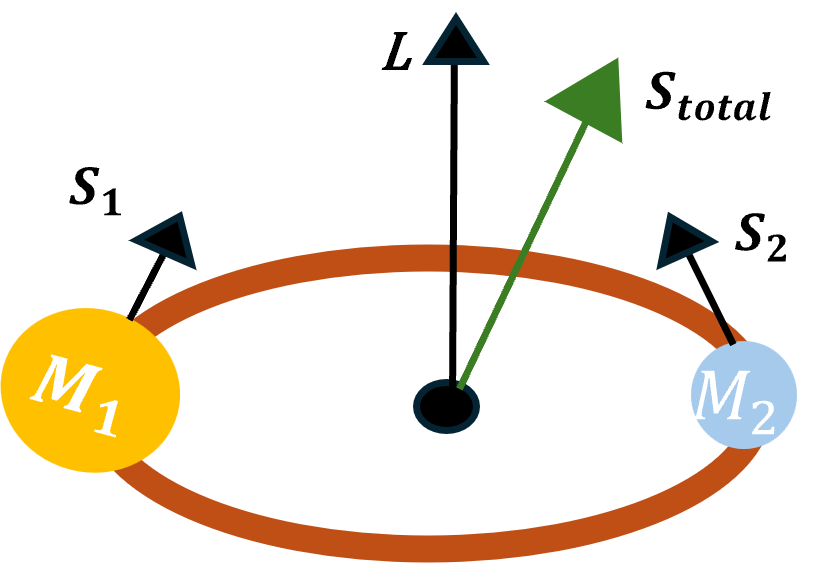
\includegraphics[width=0.4\textwidth]{LatexPlots/GRdiagram.png}
    \caption[Visualising a binary black hole system and it's intrinsic parameters]{Visualising a binary black hole system. The two black holes with masses \(M_1\) and \(M_2\) orbit each other in a quasi-circular orbit, 
    each with spin vectors \(\mathbf{S}_1\) and \(\mathbf{S}_2\). The total spin is \(\mathbf{S}_{\text{total}} = \mathbf{S}_1+\mathbf{S}_2\) and \(\mathbf{L}\) is the orbital angular momentum. 
    The spin projections \( \chi_{\parallel} \) and \( \chi_{\perp} \) are the components of the total spin that are parallel and perpendicular to \( \mathbf{L} \), respectively.}
    \label{fig:gr_diagram}
\end{figure}
To assist in training our GPR model, we begin by scaling the input parameters. The total mass is scaled to lie in the interval \([0, 1]\), with four discrete values. For each total mass, the five values for the symmetric mass ratio are scaled to span the interval \([-1, 1]\). 
We also transform the spin data \((X_{\parallel}, X_{\perp})\) onto a uniform grid of size \(10 \times 25\), with:
\[
x \in \{0.1, 0.2, \ldots, 1\}, \qquad y \in \left\{-\frac{\pi}{2},-\frac{\pi}{2}+\frac{\pi}{24},\ldots, \frac{\pi}{2}\right\}.
\]
\begin{equation}
(x, y, z, w) = \text{transformed}(X_{\perp}, X_{\parallel}, \eta, M_{\text{tot}}),
\end{equation}
where \(x\), \(y\), \(z\), and \(w\) are the scaled inputs used in our GPR framework.

    \begin{figure}[H]
        \centering
        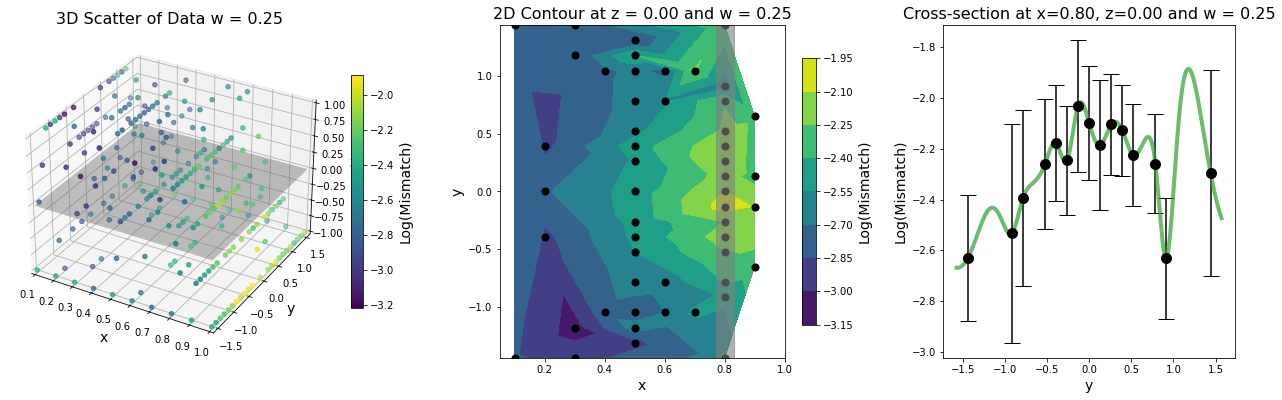
\includegraphics[width=\textwidth]{LatexPlots/final_gps_plots/data_visual.png}
        \caption[Visualisation of the input data across reduced dimensions.]{
        Visualisation of the input data across reduced dimensions. 
        Left: A 3D scatter plot of all data points for fixed total mass \(w = 0.25\) ($M_\text{tot}=37.5 M_\odot$). 
        Centre: A 2D slice of the data at rescaled symmetric mass ratio \(z = 0\) ($q=0.404$), interpolated over spin components.
        Right: A 1D cut through the data at \(x = 0.8\) showing variation across \(y\). 
        When using raw data, interpolation is needed between samples, but GPR provides an analytic model that can be directly evaluated without interpolation.
        }
        \label{fig:visualising_data}
    \end{figure}







\chapter{Gaussian Process Regression Background}
\section{Introduction and Roadmap}

In the following subsections, I discuss the following foundational concepts of Gaussian Process Regression \textbf{(GPR)}:
\begin{enumerate}
    \item \textbf{Gaussian Processes Regression Background:} Section~\ref{sec: GP_backgroound} introduces Gaussian Processes and explains how their priors and posteriors are constructed from finite sets of points.
    \item \textbf{Kernel Functions:} In Section~\ref{sec: Kernels}, I explore how kernels encode the basic assumptions about smoothness and structural properties of the underlying function. I look at how kernel hyperparameters effect the shape of samples from our prior distribution.
    \item \textbf{Noise Modeling:} Section~\ref{sec: Handlingnoise} covers several approaches for incorporating observational noise into the GP framework. I look at how noise effects the samples from our prior distribution.
    \item \textbf{Hyperparameter Optimization:} In Section~\ref{sec: Hyper_parameters}, I discuss how kernel and noise hyperparameters can be optimised resulting in a posterior distribution that better explains our data.
    \item \textbf{Hyperparameter Uncertainty:} In Section~\ref{sec: MCMC}, I discuss the uncertainty associated to the point estimates found by parameter optimisation using log-likelihood and how we can build a better predictive distribution marginalised over the hyperparameters.
    \item \textbf{Multi Dimensional GPR:} We discuss how the GPR then generalises for multiple dimensional inputs in Section~\ref{sec:multidims}.
\end{enumerate}

\section{Gaussian Proces Regression Background}
\label{sec: GP_backgroound}
\subsection{Definition of a Gaussian Process}
\label{sec: Definition_of_GP}
%
A Gaussian Process \textbf{(GP)} defines a probabilistic model over all possible functions rather than assuming a single function to be true
\begin{equation}
f(X) \sim \mathcal{GP} (\mu(X), k(X, X')).
\label{eq: Initial_GP_distribution}
\end{equation}
where \( \mu(X) \) is the mean function, specifying the expected function value at each \( X \):
\begin{equation}
    \mu(X) = {E}[f(X)],
    \label{eq: meandef}
\end{equation}
%
\( k(X, X') \) is the covariance function (kernel), encoding the relationships between function values at different points:
\begin{equation}
    k(X, X') = \text{Cov}(f(X), f(X')).
    \label{eq: kerneldef}
\end{equation}
%

Since the input space is continuous, the GP represents an infinite-dimensional distribution. 
In practice, we approximate the process by evaluating the GP at a finite set of inputs.
These function values are then assumed to follow a multivariate normal Gaussian distribution.
%
Mathematically, for a finite set of input points
\begin{equation}
X = \{X_1, X_2, \dots, X_n\},
\end{equation}
 the corresponding function values
\begin{equation}
f = \{f(X_1),f(X_2),...,f(X_n), \}
\end{equation}
follow a multivariate normal distribution
\begin{equation}
f \sim \mathcal{N}\left(\mu(X), K(X, X)\right).
\label{eq: Multivariate_distribution}
\end{equation}
Each sample from this multivariate distribution represents a function evaluated at \( n \) different points.

\subsection{The Prior Distribution}
\label{sec: prior_dist}
Before observing any data, we assume a joint Gaussian distribution over both training and test points. Let \( X \) denote training inputs and \( X_* \) test inputs. 
The joint prior over their function values is
\begin{equation}
\begin{bmatrix}
f(X) \\
f(X_*)
\end{bmatrix}
\sim \mathcal{N}
\left(
\begin{bmatrix}
\mu(X) \\
\mu(X_*)
\end{bmatrix},
\underbrace{
\begin{bmatrix}
K(X, X) & K(X, X_*) \\
K(X_*, X) & K(X_*, X_*)
\end{bmatrix}
}_{\mathcal{C} = \text{Covariance Matrix}}\right).
\label{eq: Multivariate prior}
\end{equation}
%
The corresponding joint probability density function (pdf) is given by:
%
\begin{equation}
    p(f, f_*) = \frac{1}{(2\pi)^{n/2} \sqrt{|\mathbf{C}|}} \exp\left( 
    - \frac{1}{2}\left(\begin{bmatrix}f \\f_*\end{bmatrix}-
    \begin{bmatrix}\mu(X) \\\mu(X_*)\end{bmatrix}\right)^T
    \mathbf{C}^{-1}\left(
    \begin{bmatrix}f \\f_*\end{bmatrix}-
    \begin{bmatrix}\mu(X) \\\mu(X_*)\end{bmatrix}\right)\right).
\end{equation}
%

After accounting for the mean, the resulting distribution is entirely determined by its kernel function.
The kernel governs how the model generalizes to unseen data. There are many kernel choices, each encoding different structural assumptions about the function, such as smoothness, periodicity, or linearity.
In the next section we examine the different kernel choices available and the assumptions that each kernel encodes about our function structure, such as smoothness and periodicity.



\section{Kernel Functions}
\label{sec: Kernels}
The kernel function encodes our assumptions about the relationship between input points in a Gaussian Process (GP).
It defines the covariance between any two function values and thereby determines the smoothness, periodicity, or other properties of the functions drawn from the GP prior.
Fundamentally, kernels reflect the idea of similarity: input points \( x \) and \( x' \) that are close together are assumed to have highly correlated outputs \( f(x) \) and \( f(x') \),
while distant inputs are assumed to produce less correlated values. This notion of similarity, as emphasized in \cite[Ch.~4]{bible}, is central to how Gaussian processes learn from and generalize beyond training data.
%

In Figure~\ref{fig: samples_from_GP_prior}, we illustrate the effect of the kernel on the GP prior.
We draw three functions from the multivariate Gaussian prior defined in Equation~\ref{eq: Multivariate prior}, using a zero mean and an RBF kernel.
The first subplot shows these samples, while the second subplot visualizes the corresponding covariance matrix as a heatmap.
The matrix reveals that correlations are strongest when input points are close together (near the diagonal) and decay as the distance between inputs increases.
This is evident also from the samples as we can see nearby points often move in similar directions, while distant points diverge more significantly.
%

The final three subplots highlight how this distance-based correlation manifests in the joint distribution of pairs of function values.
For closely spaced inputs, such as \( (x, x') = (0, 0.1) \), the joint distribution of \( (f(0), f(0.1)) \) forms a narrow elliptical contour,
indicating strong correlation (approximately 0.9). As the distance increases, such as in the pairs \( (0, 0.5) \) and \( (0, 1) \), the ellipses widen, reflecting weaker correlation. This visualization reinforces the intuition that kernel functions govern how input proximity translates to output similarity.

\begin{figure}[H]
    \centering
       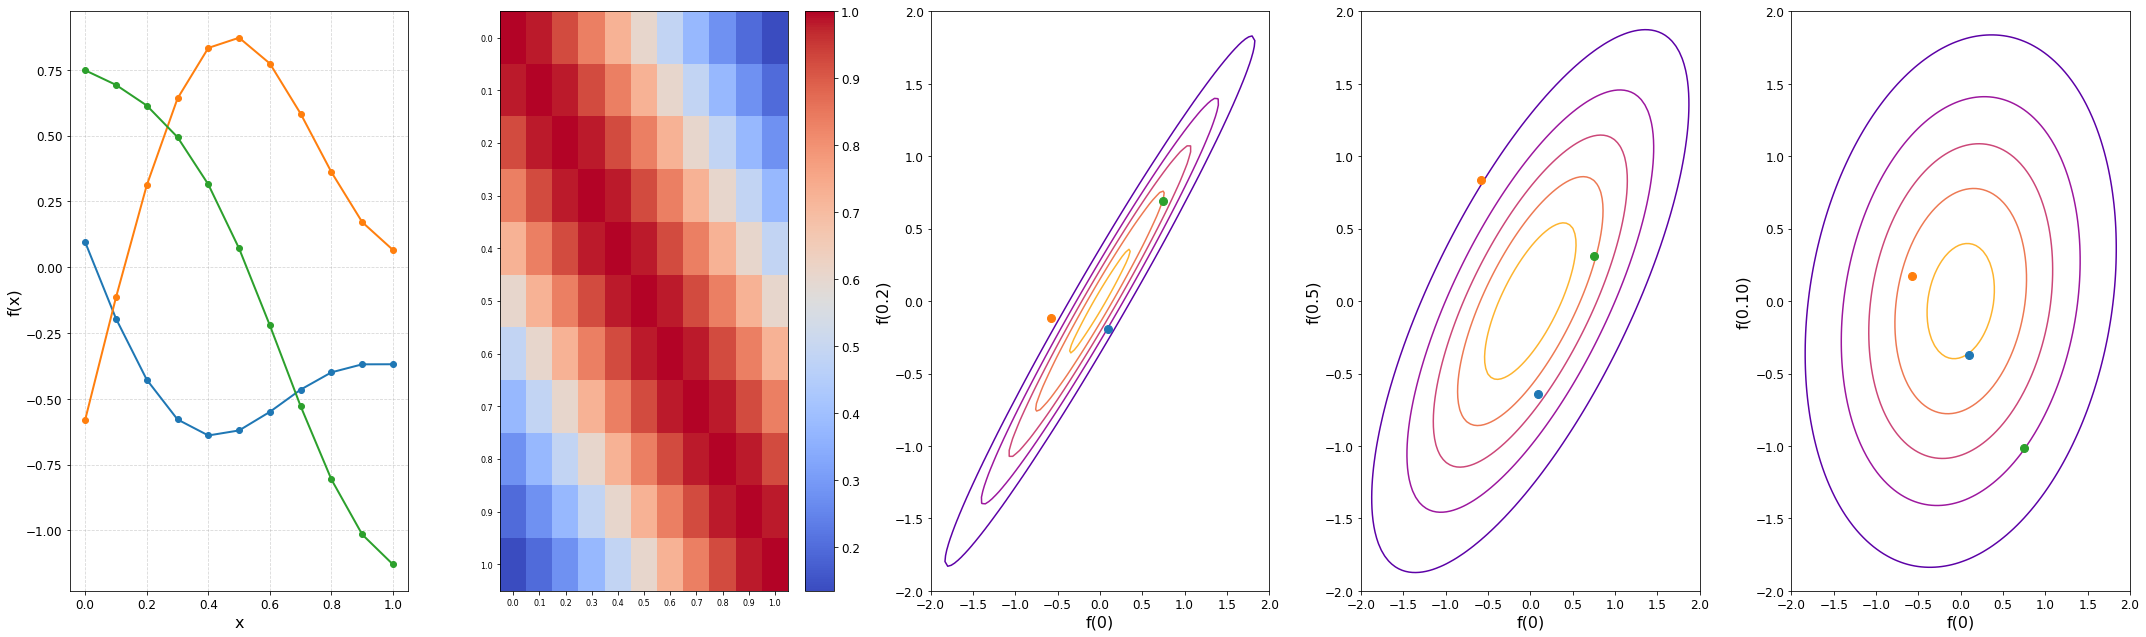
\includegraphics[width=\textwidth]{LatexPlots/1dplots/Kernel_background.png}
        \caption[Visualising the assumptions the kernel encodes into our GP process.]{Sampling from the GP prior with zero mean and an RBF kernel ($\ell = 0.5$, $\sigma_f^2 = 1$). 
        The first plot shows three sample functions drawn from the prior distribution. 
        The second plot visualizes the covariance matrix as a heatmap, revealing the strength of correlations between inputs.
        The final three subplots display joint distributions between selected input pairs. These distributions are multivariate distributions with mean zero and covariance matrix defined by a \(2 \times 2\) where the diagonals are 1 and the off diagonals are the correlation between the selected input points.
        The contours are drawn at multiples of \(0.5 \sigma\) indicating confidence regions for each distribution}
    \label{fig: samples_from_GP_prior}
\end{figure}
%

We have discussed how the kernel function encodes the covariance structure of the GP prior. This structure depends on the choice of kernel. According to \cite{bible}
kernels can be divided into two major sub-groups, stationary kernels and non-stationary kernels. 
Stationary kernels depend only on the relative (often radial) distance between inputs \(\|x - x'\|\) and are invariant to translations 
in the input domain. By contrast, non-stationary kernels depend explicitly on 
the absolute values of \(x\) and \(x'\), allowing the function’s properties—such as smoothness 
or amplitude—to vary across the domain. For more detailed discussion on building, combining, and customizing these kernels, 
see \cite{kernelcookbook} and \cite[Ch.~4]{bible}.
%

In Table~\ref{tab:kernel-examples}, we provide an overview of several common kernel types, 
showing both their functional form and samples drawn from the corresponding GP priors. 
While each kernel imposes a distinct structural pattern on the functions—such as smoothness, periodicity, or linearity—they are all similarly influenced by shared hyperparameters like the lengthscale. 
In addition, many kernels include unique internal parameters that further shape the behaviour of the modeled functions. 
In the following subsections, we explore each of these kernels in detail and discuss the role of their associated hyperparameters.
%

\begin{table}[H]
    \centering
    \renewcommand{\arraystretch}{4} % Slightly tighter rows
    \setlength{\tabcolsep}{0.5pt} % Tighter columns
    \small % Smaller text to fit content
    {\fontsize{6}{9.5}\selectfont
    \begin{tabular}{|>{\centering\arraybackslash}m{1.85cm}|*{6}{>{\centering\arraybackslash}m{2.3cm}|}} 
        \hline
        \textbf{Kernel name:} & \textbf{RBF (SE)} & \textbf{Rational Quadratic} & \textbf{Periodic} & \textbf{Matern} & \textbf{Laplace} & \textbf{Linear (Dot Product)} \\ 
        \hline
        \textbf{Plot of $k(x, x')$:} & 
        \adjustbox{valign=c}{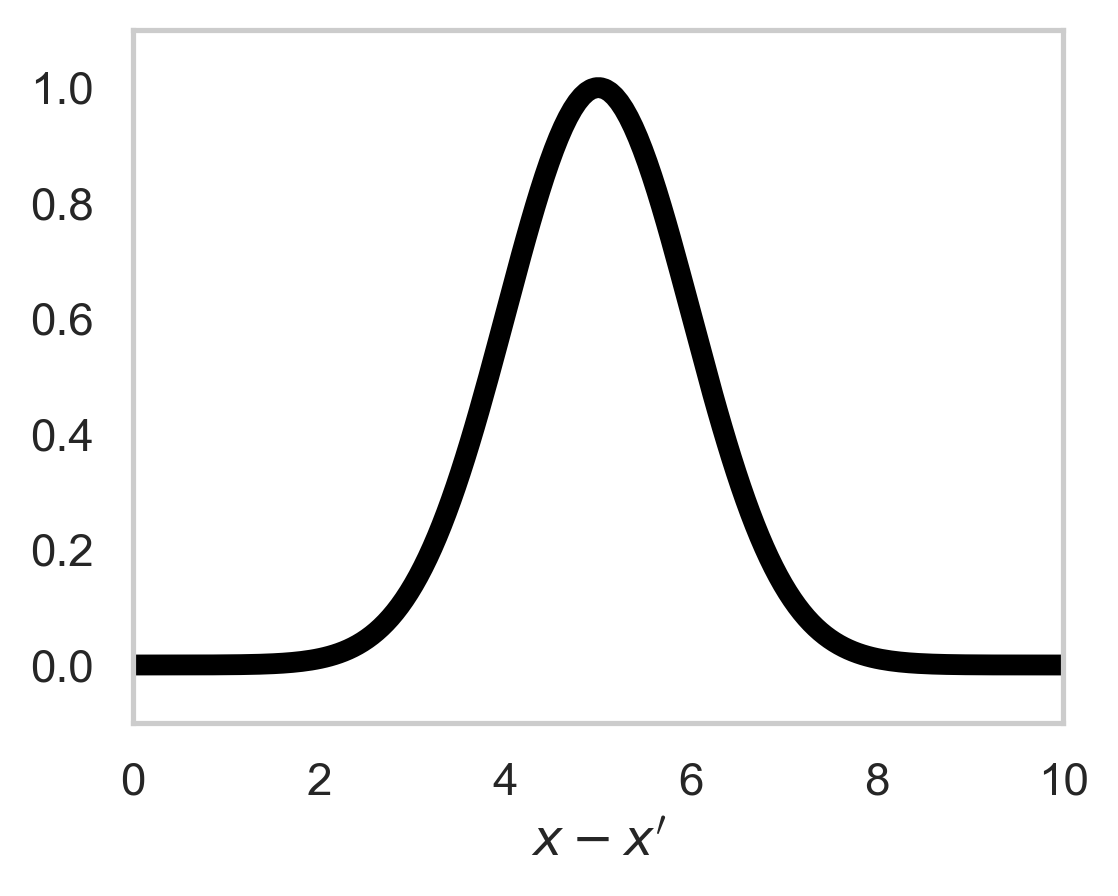
\includegraphics[width=2cm]{LatexPlots/1dplots/Kernel_RBF_SE.png}} & 
        \adjustbox{valign=c}{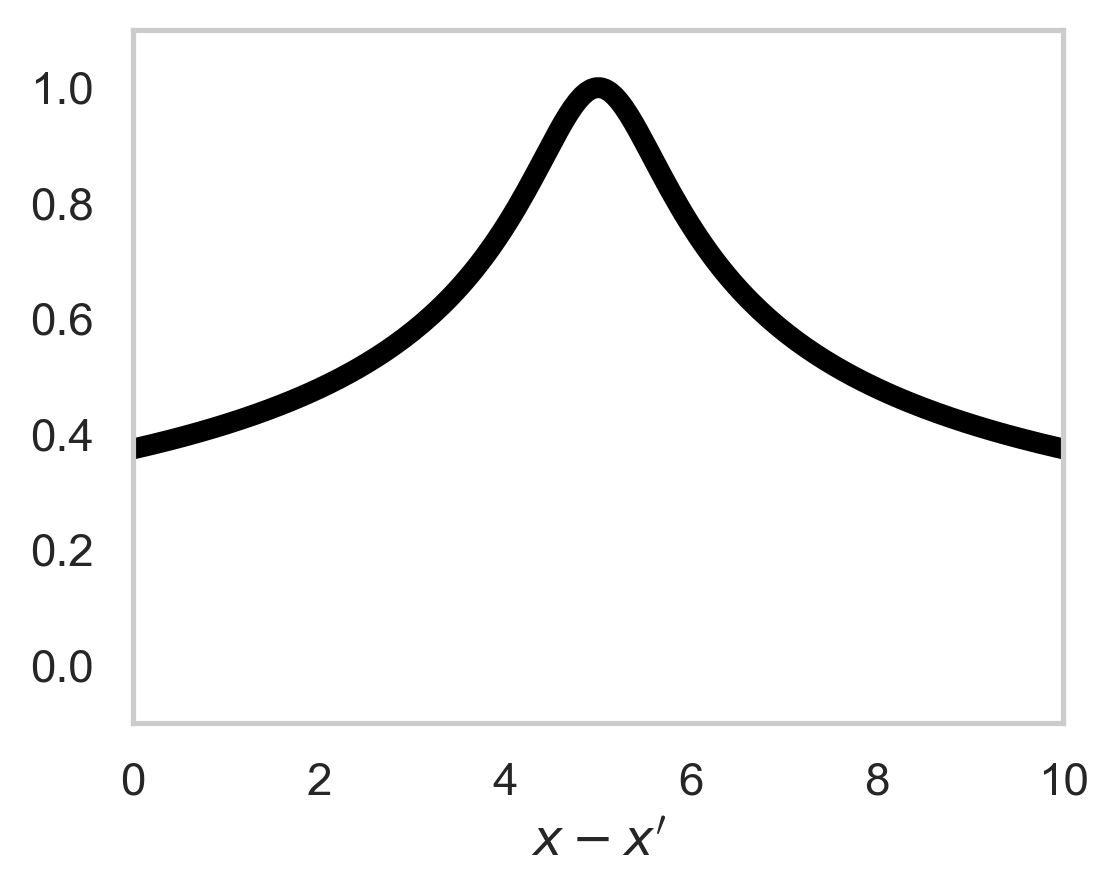
\includegraphics[width=2cm]{LatexPlots/1dplots/Kernel_Rational_Quadratic.png}} & 
        \adjustbox{valign=c}{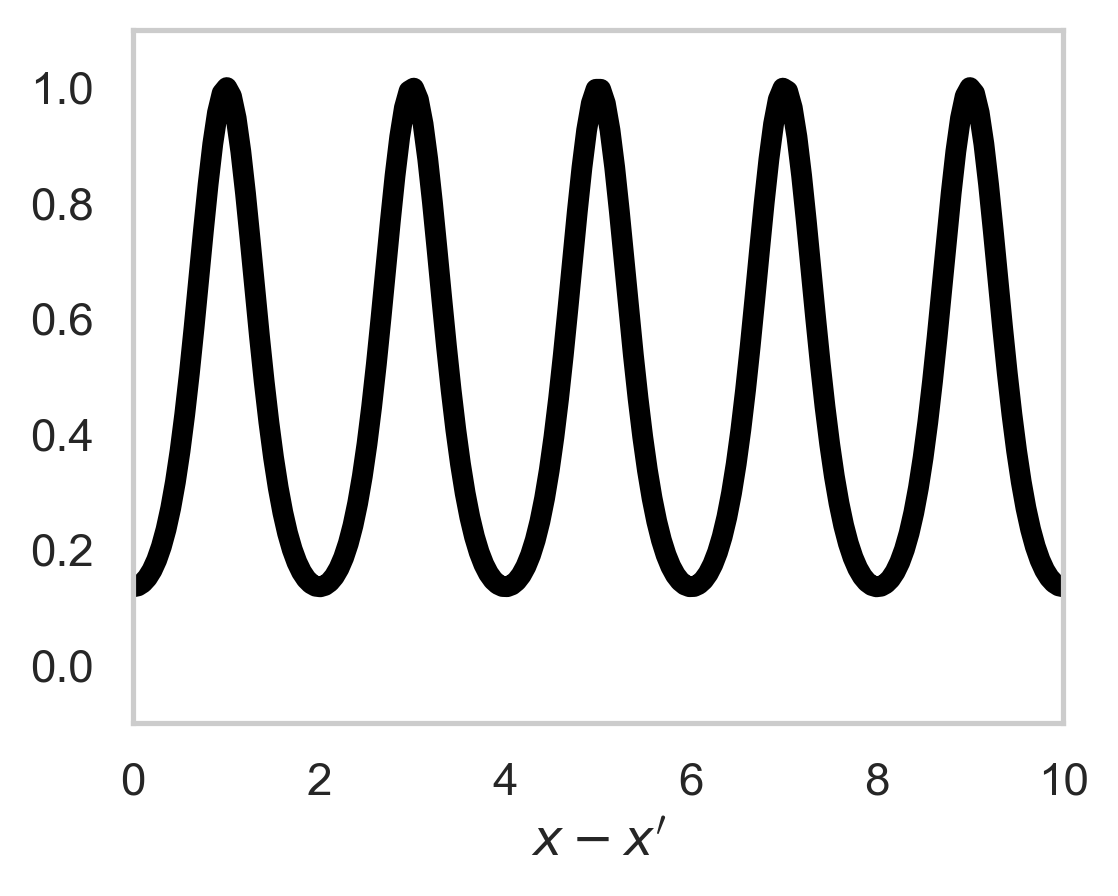
\includegraphics[width=2cm]{LatexPlots/1dplots/Kernel_Periodic.png}} & 
        \adjustbox{valign=c}{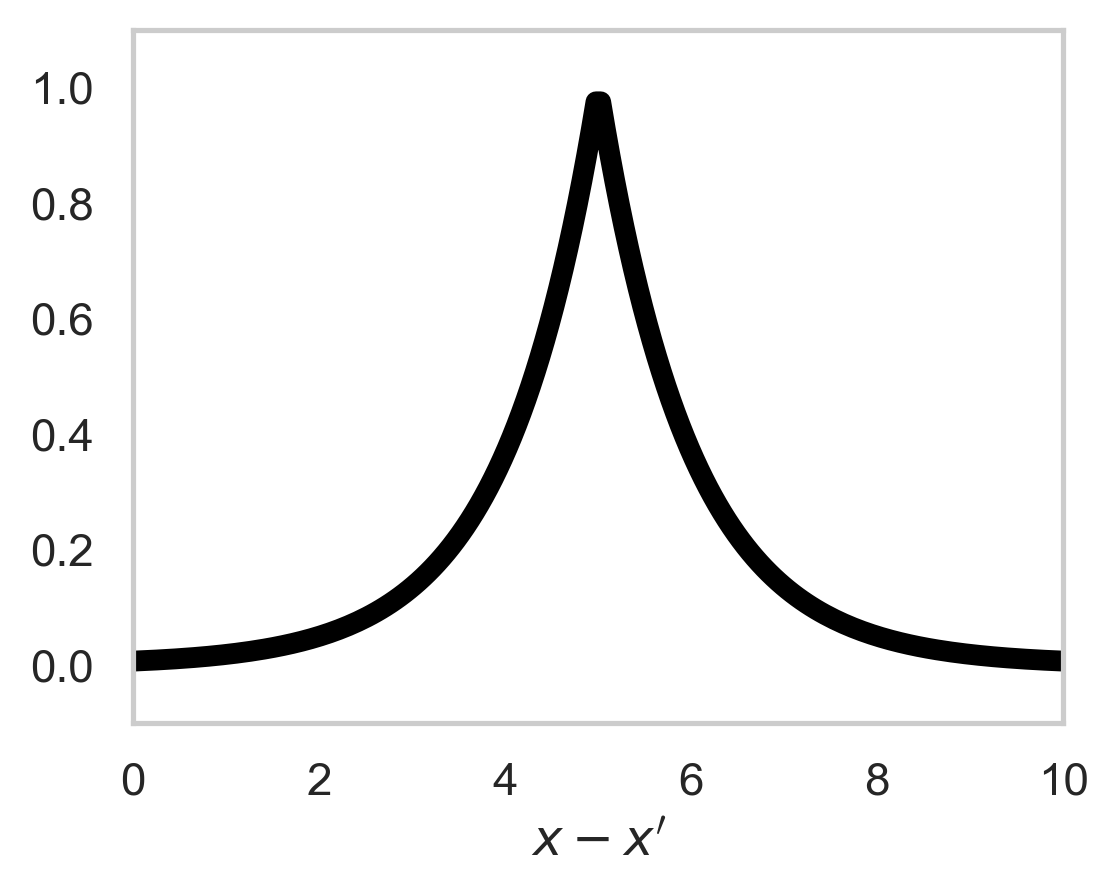
\includegraphics[width=2cm]{LatexPlots/1dplots/Kernel_Matern_nu05.png}} & 
        \adjustbox{valign=c}{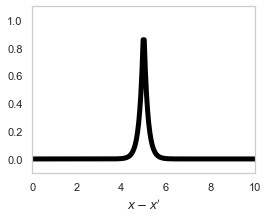
\includegraphics[width=2cm]{LatexPlots/1dplots/Kernel_Laplace_Exponential.png}} & 
        \adjustbox{valign=c}{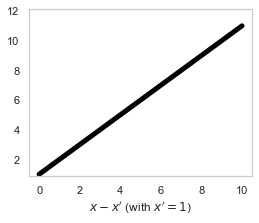
\includegraphics[width=2cm]{LatexPlots/1dplots/Kernel_Linear_Dot_Product.png}} \\ 
        \hline
        \textbf{GP Prior Samples:} & 
        \adjustbox{valign=c}{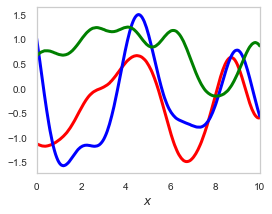
\includegraphics[width=2cm]{LatexPlots/1dplots/KernelSample_RBF_SE.png}} & 
        \adjustbox{valign=c}{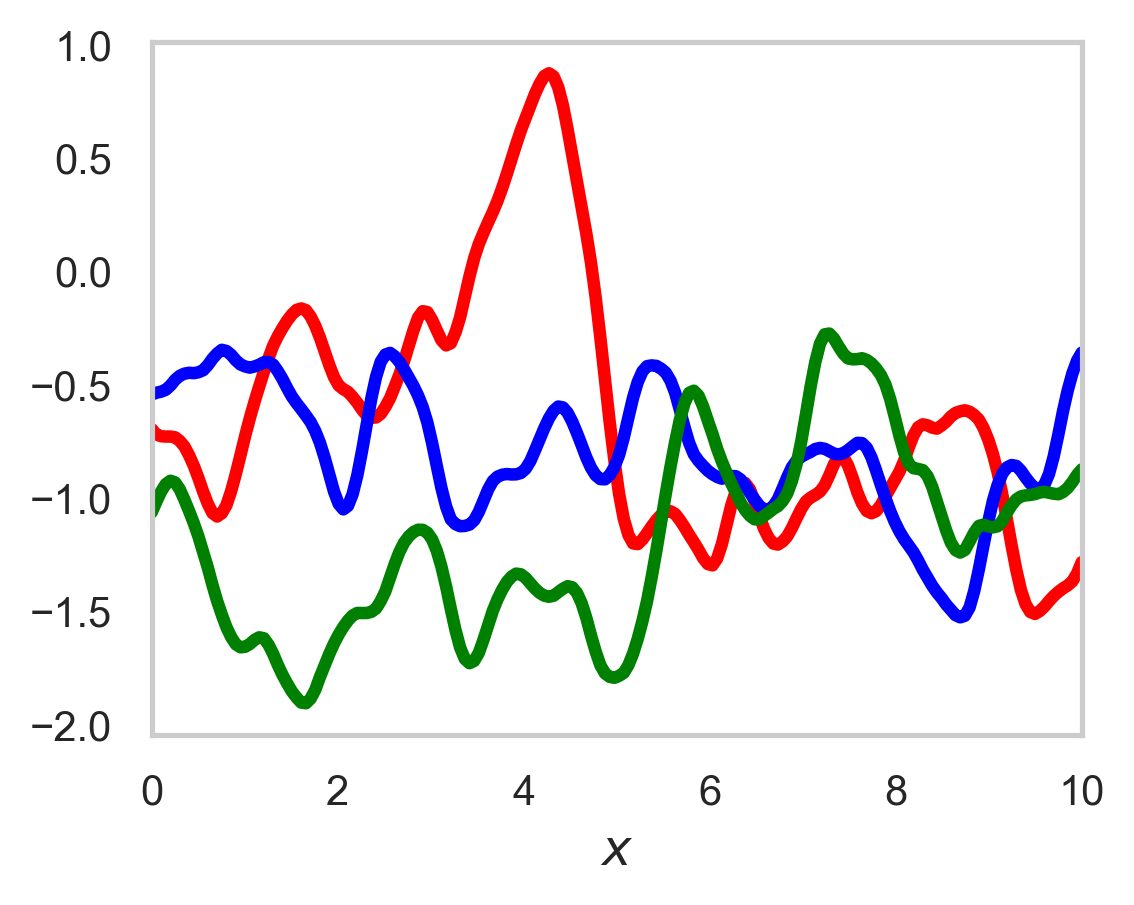
\includegraphics[width=2cm]{LatexPlots/1dplots/KernelSample_Rational_Quadratic.png}} & 
        \adjustbox{valign=c}{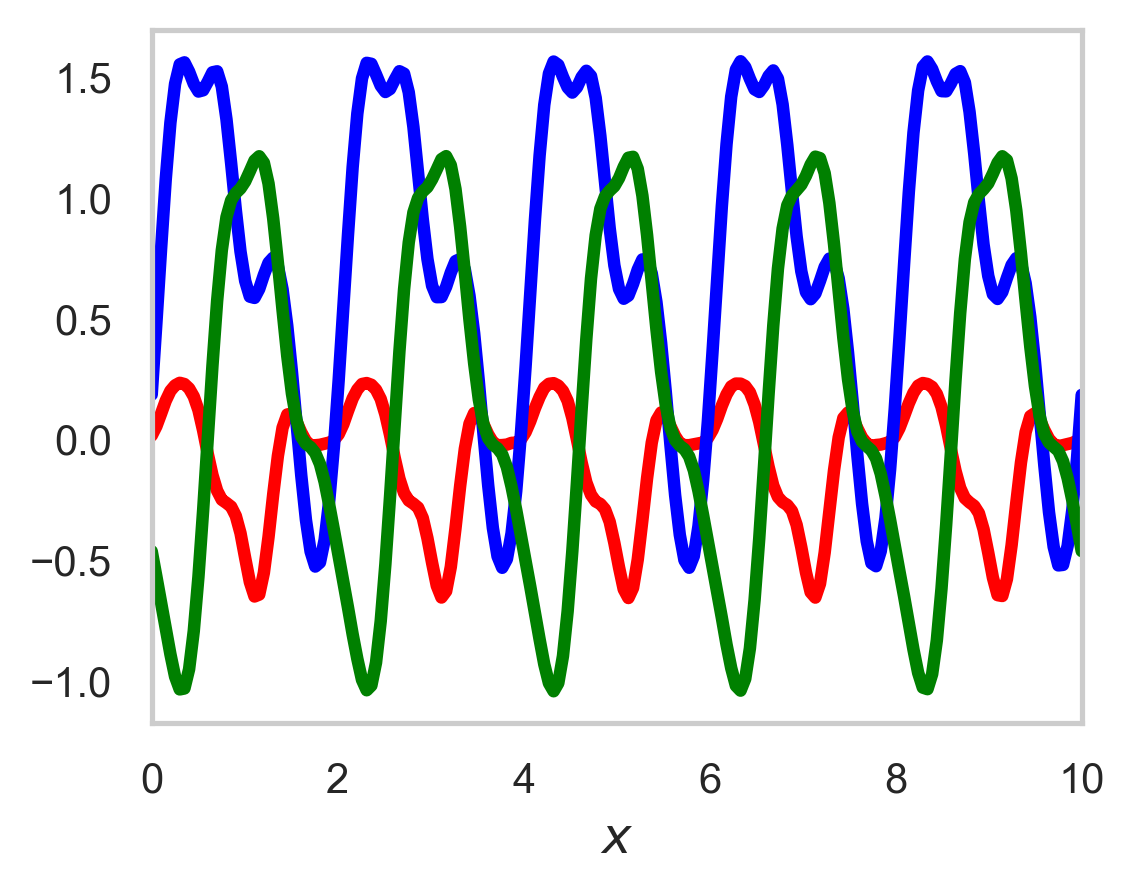
\includegraphics[width=2cm]{LatexPlots/1dplots/KernelSample_Periodic.png}} & 
        \adjustbox{valign=c}{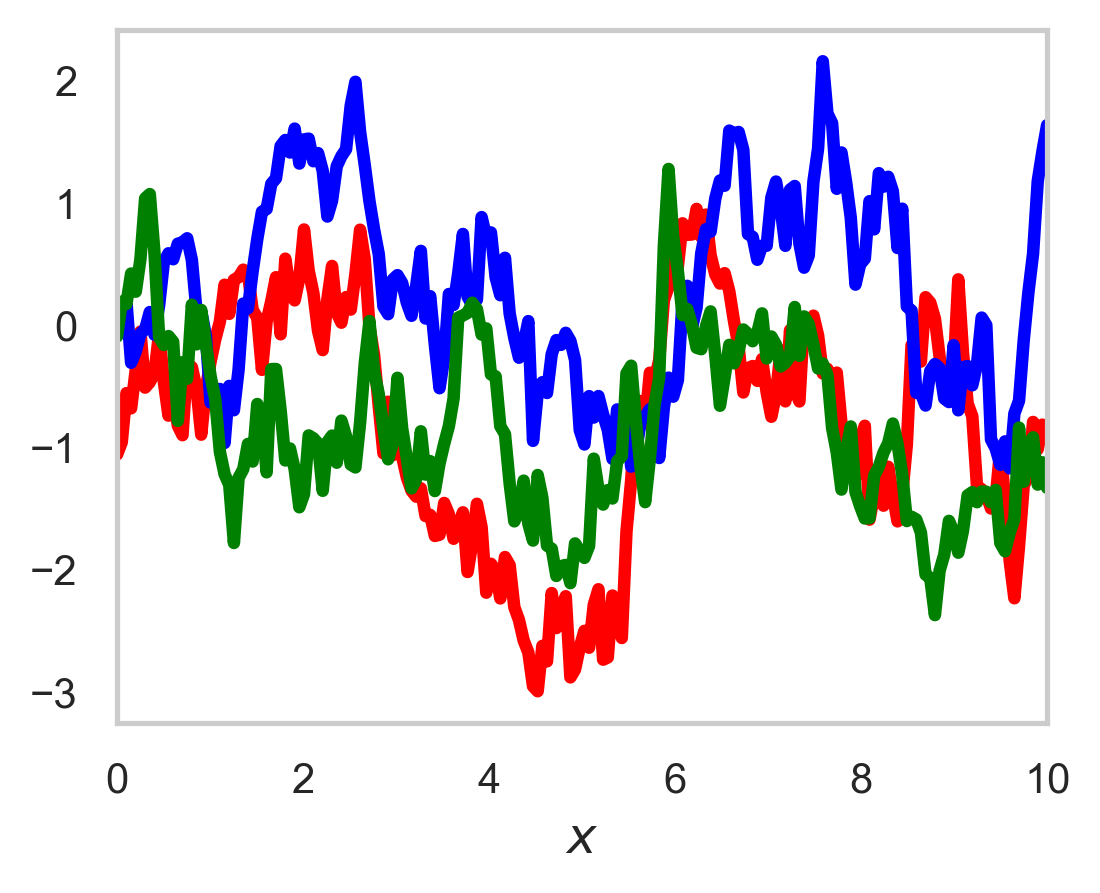
\includegraphics[width=2cm]{LatexPlots/1dplots/KernelSample_Matern_nu05.png}} & 
        \adjustbox{valign=c}{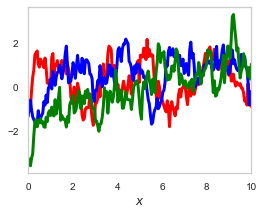
\includegraphics[width=2cm]{LatexPlots/1dplots/KernelSample_Laplace_Exponential.png}} & 
        \adjustbox{valign=c}{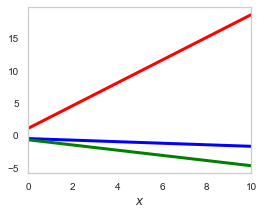
\includegraphics[width=2cm]{LatexPlots/1dplots/KernelSample_Linear_Dot_Product.png}} \\ 
        \hline
        \textbf{Key Hyperparameters} &
        $\ell$ (Lengthscale) &
        \shortstack{$\ell$ \\ $\alpha$ (Scale-mix)}&
        \shortstack{$\ell$ \\ $p$ (Period)} &
        \shortstack{$\ell$ \\ $\nu$ (Smoothness)} &
        $\gamma$ (Decay rate) &
        None or variance \\ 
        \hline
        \textbf{Structure type:} & 
        Local variation & 
        Multi-scale local variation & 
        Repeating structure & 
        Rough to smooth & 
        Rougher variation & 
        Linear functions \\ 
        \hline
    \end{tabular}}
    \caption[Visual comparison of common kernel functions and their effect on Gaussian process priors. ]{
        Visual comparison of common kernel functions and their effect on Gaussian process priors. 
        Each column shows the kernel shape $k(x, x')$, samples from the corresponding GP prior, and a summary of the structure it imposes. 
        All kernels were evaluated using a lengthscale parameter $\ell = 1$ (except where noted). 
        For the Matern kernel, $\nu = 0.5$; Laplace kernel, $\gamma = 6$; Rational Quadratic kernel, $\alpha = 0.25$; and Periodic kernel, period $p = 2$.
        Detailed formula each kernel are provided in the appendix \ref{appendix:B}.Note: In practice, we scale each kernel by a signal variance hyperparameter \(\sigma_f^2\), which governs the overall vertical variation in the function.
        This scaling is applied consistently across all kernel types and accounts for the amplitude of the wave.
        }
    \label{tab:kernel-examples}
\end{table}
%

From Table~\ref{tab:kernel-examples}, we observe that the RBF, Rational Quadratic, Matern, Laplace, and Periodic kernels are all examples of stationary kernels (i.e depend on $|x-x'|$). 
Many of these, such as the RBF, Matern,Rational Quadratic and Laplace, exhibit ``bell-shaped'' structures. Their inputs \(x\) and \(x'\) that are close together yield high covariance,
which then decays as the distance \(\|x - x'\|\) increases. The Periodic kernel, while also stationary, has a unique structure. Instead of decaying monotonically with distance, 
it assigns high covariance to inputs that are separated by integer multiples of a fixed period \(p\). This leads to the kernel encoding a periodic pattern on the sampled functions.
%

Having examined multiple kernel types and their properties we will now examine the effect of the kernel hyper-parametrs \(\ell,\sigma_f^2\) on the GP prior. 
In Figure~\ref{fig: GPprior_hyperparams} we see that small \(\ell\) results in samples that are noisy with lots of local variations. This is beacuse the rate of decrease of the covariance
between points is determined by \(\ell\) and so small \(\ell\) reinforces that only points very close to \(x'\) are correlated with \(x'\). However the larger \(\ell\) gets the 
more correlation \(x'\) has with further points therefore resulting in smooth curves.
Visualising the effect of the signal variance \(\sigma_f^2\) we can see that simply larger \(\sigma_f^2\) results in the vertical variation of each sample becoming bigger.
%

\begin{figure}[H]
    \centering
        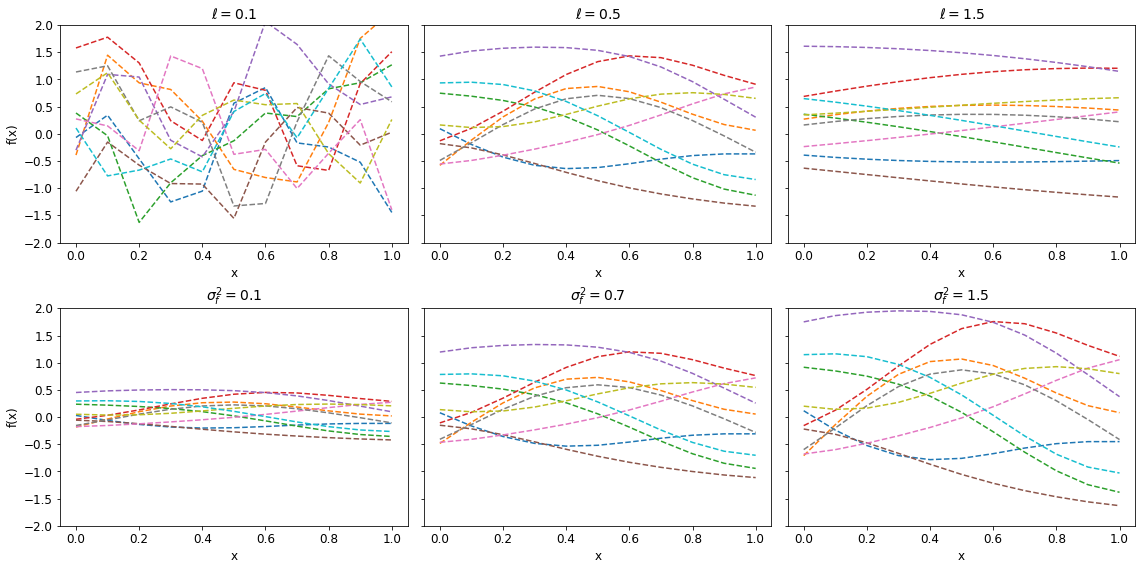
\includegraphics[width=\textwidth]{LatexPlots/1dplots/Kernel_hyperparams.png}
        \caption[Visualising the effect of kernel hyperparameters.]{Sampling from the GP prior with mean 0 and covariance given by the RBF kernel.
        The first plot shows the effect of the lengthscale hyperparameter \(\ell\) on the GP prior.We fix the signal variance to 1.
        The second plot shows the effect of the signal variance hyperparameter \(\sigma_f^2\) on the GP prior.We fix the lengthscale to 0.5.}
    \label{fig: GPprior_hyperparams}
\end{figure}

\section{Building the Posterior Distribution}
\label{sec: priortoposterior}

We have discussed how our prior distribution is dependent on the choice of kernel and the hyperparameters of said kernel. In this section
we will discuss how we can update our prior distribution \ref{eq: Multivariate prior} to achieve our new prediction distribution distribution from which we can make
inferences. One of the key strengths of Gaussian Processes is that, given observations at training inputs \(X\) and setting kernel hyperparameters \(\theta\)
we can make predictive inferences about the function value at any new test location \(x_*\).
By applying the standard conditional Gaussian formulas (see appendix \todo{clean appendoix} \ref{appendix:A} for the full derivation),
the posterior distribution of \(f(x_*)\) given \(\{X, f(X)\}\) is Gaussian and given by:
%
\begin{subequations}
    \begin{equation}
    p\bigl(f(x_*) \mid f(X), X, X_*,\theta \bigr) 
    \sim \mathcal{N}\!\left(m(x_*),\;\sigma^2(x_*)\right),
    \end{equation}
    \vspace{-8ex}
    \begin{align}
    m(x_*) 
    &= \mu(x_*) + k(x_*, X)\,k(X, X)^{-1}\left[f(X) - \mu(X)\right],
    \label{eq: predictive_mean} \\
    \sigma^2(x_*) 
    &= k(x_*, x_*) - k(x_*, X)\,k(X, X)^{-1}\,k(X, x_*).
    \label{eq: predictive_variance}
    \end{align}
    \label{eq: predictive_dist}
\end{subequations}    
% 
In these expressions:
\begin{itemize}
    \item \( \mu(\cdot) \) is the mean function ( We take this to be zero since we centre the data prior to prediction),
    \item \( k(X, X) \) is the covariance matrix among the observed training points,
    \item \( k(x_*, X) \) is the vector of cross-covariances between the test point \(x_*\) and the training inputs,
    \item \( k(x_*, x_*) \) is the prior variance at the test point itself.
\end{itemize}
%

We now have an analytic function that can be evaluated to find the mean function value and variance at any input point.
This is a very useful property that Gaussian Processes possess. Figure~\ref{fig: priortoposterior} shows how we update our
distributions based on the training points. We initially plot samples taken from the prior distribution (Equation~\ref{eq: Multivariate prior}). 
After conditioning this distribution on one training point and obtaining the new predictive posterior distribution (Equation~\ref{eq: predictive_dist}), 
we see that the predictive mean passes exactly through the training point, has small variance around it, and then fans out farther away. 
Conditioning on two training points at opposite ends of our input domain creates an ellipse-shaped credible interval whose largest radius 
appears midway between the two training points. With more training points, the predictions align progressively closer to the true function 
and the variance becomes smaller.
%

Note that this example uses a one-dimensional, noise-free function and a basic RBF kernel with fixed hyperparameters (\(\ell = 1\), \(\sigma^2 = 0.5\)). 
In practice the choice of Kernel function plays a pivotal role in the assumptions we make about the shape and general behaviour of our model. In the next section
we examine the different kernel choices available and the assumptions that each kernel encodes about our function structure, such as smoothness and periodicity.


\begin{figure}[H]
    \centering
    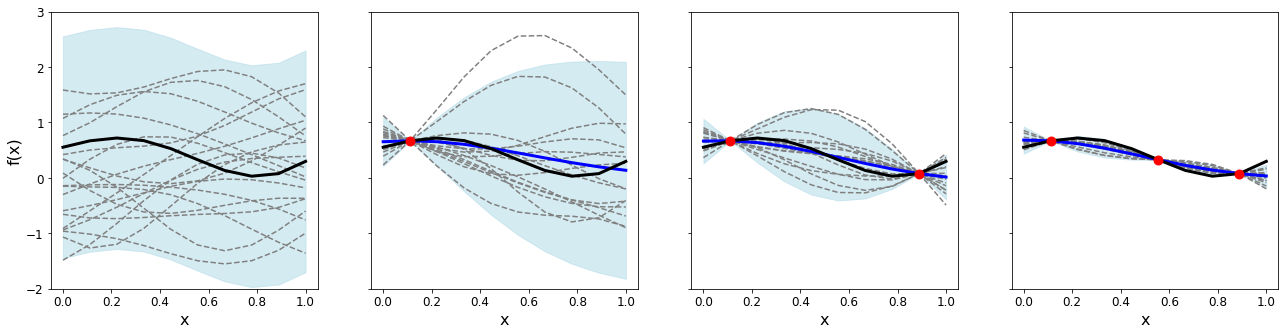
\includegraphics[width=\textwidth]{LatexPlots/1dplots/priortoposterior.png}
    \caption[Building the posterior distribution]{1D Gaussian Process Regression: Prior to Posterior. This sequence shows how the GP prior transforms into a posterior as more data points are added. 
    The RBF kernel was used with hyperparameters: $l = 1$, $\sigma^2 = 0.5$.The black line represents the true function. The blue is the mean of each posterio distribution. 
    The light blue shaded region is the credible interval and the grey lines are the samples drawn from each posterior/prior. }
    \label{fig: priortoposterior}
\end{figure}
\todo{add a  link to animation here illustrating the nice distribution formed at each point}




\section{Handling Noise in our Data}
\label{sec: Handlingnoise}
So far, our discussion has assumed noise-free observations. However, real-world data is rarely clean, measurements often include some form of uncertainty. To make our Gaussian Process models more applicable to this real-world data,
we now explore how to incorporate noise into the GP framework.
%

We assume that each observation includes the true function value plus Gaussian noise:
\begin{equation}
y_i = f(x_i) + \epsilon_i, \quad \epsilon_i \sim \mathcal{N}(0, \sigma_{n,i}^2),
\end{equation}
where \( \sigma_{n,i}^2 \) is the noise variance associated with input \( x_i \). This allows us to model both homoscedastic and heteroscedastic noise under a unified notation.
Under this model, we have the following Gaussian assumptions:
\begin{align}
f &\sim \mathcal{N}(0, K), &&\text{(prior over the true function)}, \\
y &\sim \mathcal{N}(0, K + \Sigma), &&\text{(distribution over noisy observations)},
\label{eq: prior_distribution_noise}
\end{align}
where \( \Sigma = \mathrm{diag}(\sigma_{n,1}^2, \sigma_{n,2}^2, \dots, \sigma_{n,n}^2) \) is the noise covariance matrix.
%

This now updates our previous posterior distribution (Eqns: \ref{eq: predictive_dist}) to a revised posterior:
%
\begin{subequations}
\begin{align}
    P(f_*|X,X_*,\theta,y) &\sim \mathcal{N}(m(f_*), \text{Var}(f_*)),\\
m(f_*) &= K_*^T (K_y)^{-1} y,
\label{eq: predictive_mean_noise}\\
\text{Var}(f_*) &= K_{**} - K_*^T (K_y)^{-1} K_*,
\label{eq: predictive_variance_noise}
\end{align}
\label{eq: predictive_distribution_noise}
\end{subequations}
%
where \(K_y\) depends on how we handle our noise. There are three main cases of how we handle our noise

\subsection{Homoscedastic Noise} 

In the homoscedastic case, we assume that all observations have the same noise level, meaning the noise variance is constant across the dataset:
\[
\sigma_{n,i}^2 = \sigma_n^2 \quad \forall i.
\]
This simplifies the noise covariance matrix \( \Sigma \) to a scalar multiple of the identity matrix:
\[
\Sigma = \sigma_n^2 I.
\]
The total covariance matrix of the observed data becomes:
\[
K(X, X) + \sigma_n^2 I = 
\begin{bmatrix}
k(x_1, x_1) + \sigma_n^2 & \cdots & k(x_1, x_n) \\
\vdots & \ddots & \vdots \\
k(x_n, x_1) & \cdots & k(x_n, x_n) + \sigma_n^2
\end{bmatrix}.
\]
Our prior distribution now becomes:
\begin{equation}
y \sim \mathcal{N}(0, K+\sigma_n^2 I),
\label{eq: prior_withnoise}
\end{equation}
where $\sigma_n^2$ is a new parameter which effects the shape of the distribution. In figure \ref{fig: GPprior_hyperparams} we 
explored how the internal kernel hyperparameters effect the shape of the sampes from our prior distribution. We now examin how the noise (i.e $\sigma_n^2$) effects samples from our prior distribution from \ref{eq: prior_withnoise}.
Our posterior distribution is as in eqn \ref{eq:  predictive_distribution_noise} with \(K_y = K(X, X) + \sigma_n^2 I \) for some constant \(\sigma_n\)

\begin{figure}[H]
    \centering
        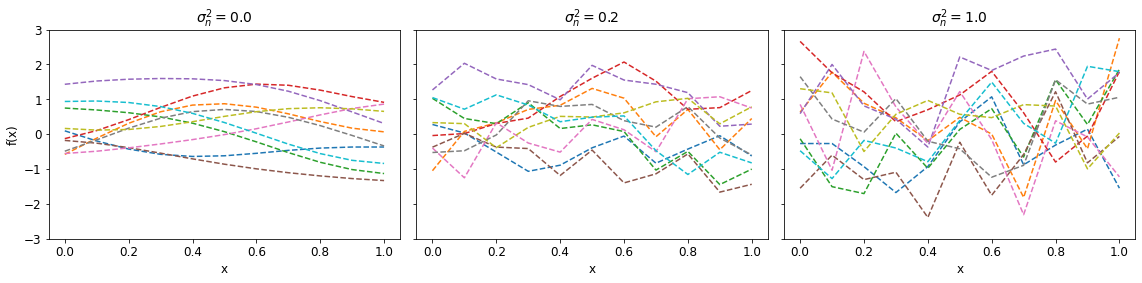
\includegraphics[width=\textwidth]{LatexPlots/1dplots/Kernel_noise.png}
        \caption[Visualising the effect of noise on samples from the GP prior.]{Sampling from the GP prior with mean 0 and covariance given by the RBF kernel.
        The plot shows the effect of the noise hyperparameter \(\sigma_n^2\) on the GP prior.We fix the signal variance to 1 and length scale to 0.5.}
    \label{fig: kernel_noise}
\end{figure}



\subsection{Heteroscedastic Noise}  
\subsubsection{Known Noise:}
%
In this case, the noise variance changes across the input space—some observations are noisier than others. If we know the individual noise variances \( \sigma_i^2 \) for each training input \( x_i \), we incorporate them by adding a diagonal noise matrix to the kernel:
\[
K(X, X) + \Sigma = 
\begin{bmatrix}
k(x_1, x_1) + \sigma_1^2 & \cdots & k(x_1, x_n) \\
\vdots & \ddots & \vdots \\
k(x_n, x_1) & \cdots & k(x_n, x_n) + \sigma_n^2
\end{bmatrix},
\]
where \( \Sigma = \text{diag}(\sigma_1^2, \sigma_2^2, \dots, \sigma_n^2) \).
In this case the noise is not found as a hyperparameter but instead just added to the diagonal of the covariance matrix.
Our posterior distribution is as in eqn \ref{eq:  predictive_distribution_noise} with \(K_y =K(X, X) + \Sigma \) where \(\Sigma\) is the known noise of our data. 
%
\subsubsection{Learning Noise over the Input Space:}
%
If the noise variance is unknown but varies across the input space, we can model it as a function. 
This is done by building a kernel that captures both smooth, global trends and rough, local fluctuations. 
In practice, this means building an additive kernel made up of sub-kernels.For example, as seen in Table~\ref{tab:kernel-examples}, some kernels like the Matern, Laplacian, or Rational Quadratic capture local variations well (interpreted as noise),
while others like the RBF capture broader, smoother structure. By combining these, we can allow one kernel component to model the general structure of the function, and the other to model the heteroscedastic noise behavior. 
Our posterior distribution is as in eqn \ref{eq:  predictive_distribution_noise} with :

\begin{equation}
    K_y = \theta_1 K_1(X, X) + \theta_2 K_2(X, X),
    \label{eq:additive_kernel}
\end{equation}
where \( K_1 \) and \( K_2 \) are distinct kernels chosen to capture different aspects of the data. 
The coefficients \( \theta_1 \) and \( \theta_2 \) are parameters that control the relative contribution of each kernel component.

\subsection{Monte Carlo Sampling of Noise}  

This technique can be applied in both homoscedastic and heteroscedastic noise settings. Rather than explicitly modelling observation noise by adding a noise term to the kernel matrix, we instead account for uncertainty by perturbing the observed outputs with sampled noise.
Assuming Gaussian noise, we generate multiple noisy versions of the observed data by sampling from our noise distribution defined by the known noise. For each of these sampled datasets, we compute a Gaussian Process posterior, and then average the predictions to obtain a final predictive distribution that integrates over observation noise.
This Monte Carlo-style approach allows uncertainty in the outputs to be naturally incorporated into the predictions without modifying the covariance structure directly. A full mathematical description of this method is provided in Appendix~\ref{appendix:monte_carlo}.

%
%
\subsection{Comparing Noise Models}
From Figure~\ref{fig:noise_comparison} we see how different noise assumptions influence samples drawn from the Gaussian Process prior. 
In the homoscedastic case (left), our samples exhibit consistent fluctuations across the entire domain due to a constant noise variance applied uniformly to all inputs. 
The heteroscedastic case (middle) introduces input-dependent noise, this results in regions of smoothness followed by abrupt variations—reflecting the fact that each output has its own associated noise level.
Finally, in the Monte Carlo noise sampling approach (right), we generate multiple samples by adding different levels of noise to our prior distribution on our true function values.
This highlight all the plausible functions consistent with the observed data and captures the full range of uncertainty introduced by noisy observations.

\begin{figure}[H]
    \centering
    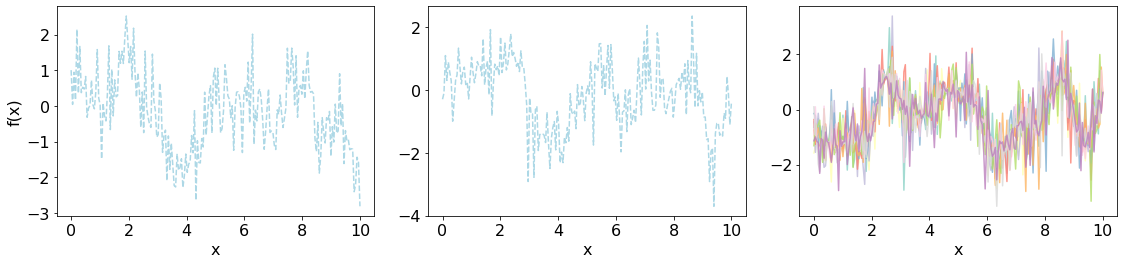
\includegraphics[width=\textwidth]{LatexPlots/1dplots/GPR_noise_comparison.png}
    \caption[Comparing samples taken from a GP with Homoscedastic noise,Heterscedastic noise and monte carlo sampling of the noise.]{Samples drawn from a zero-mean Gaussian Process prior with varying noise assumptions.
    \textbf{Left:} Homoscedastic noise, where a constant noise variance \(\sigma_n^2 = 0.5\) is added uniformly across all inputs.
    \textbf{Middle:} Heteroscedastic noise, where individual noise variances \(\sigma_i^2\) are known and drawn from \(\mathcal{N}(0, 0.5)\), resulting in a diagonal noise covariance.
    \textbf{Right:} Monte Carlo sampling of noisy observations, where multiple noisy realizations are generated from \(\mathcal{N}(f(x), \epsilon^2)\)}
    \label{fig:noise_comparison}
\end{figure}




\section{Hyperparameters}
\label{sec: Hyper_parameters}
Until now, the predictive distributions (Eqns~(\ref{eq: predictive_distribution_noise},\ref{eq: predictive_dist})) have been conditioned on fixed kernel hyperparameters. 
As shown in Figures~\ref{fig: GPprior_hyperparams} and~\ref{fig: kernel_noise}, 
these hyperparameters significantly shape both the prior and posterior behaviour of the Gaussian Process.
 However, they are not known prior to prediction and must be inferred from data. To do this, we maximize the log marginal likelihood \cite[Ch.~5]{bible}.

From Eqn~\ref{eq: prior_withnoise}, our observed data is distributed as: 
\[
y \sim \mathcal{N}(0, K + \Sigma I),
\]
the corresponding marginal likelihood for a multivariate Gauusian distribution is:
\[
p(y \mid X, \theta) = \frac{1}{(2\pi)^{n/2} \,\lvert K_y \rvert^{1/2}} 
\exp\!\Bigl(-\tfrac12\,y^\top K_y^{-1} y\Bigr), 
\quad\!\text{where}\quad K_y = K + \Sigma I.
\]
Taking the logarithm yields:
\begin{equation}\label{eq: 5}
\log p(y \mid X, \theta) 
= -\tfrac{1}{2}\,y^\top K_y^{-1}y \;-\; \tfrac{1}{2}\,\log\lvert K_y \rvert \;-\; \tfrac{n}{2}\,\log 2\pi.
\end{equation}
Optimizing this with respect to \(\theta\) provides hyperparameter estimates for kernel lengthscales, 
variances, and (if applicable) noise levels. Once these estimates are obtained, we can make accurate posterior predictions.

Figure~\ref{fig:Optimising_Hyperparams} plots the log marginal likelihood over different hyperparameter pairs. In several panels, the surface flattens at its peak indicating that multiple 
hyperparameter combinations yield nearly the same log likelihood.
The final 3D scatter plot zooms in on the region surrounding the optimiser's point estimate,
the similar shading near the black dot (the point estimate) illustrates how small variations in \(\theta\) can produce very similar likehood values. 
This flatness in the likelihood surface leads to difficulty in choosing a true optimal point and leads to uncertainty in our model. 
This will be further discussed in the following section.

\begin{figure}[H]
    \centering
    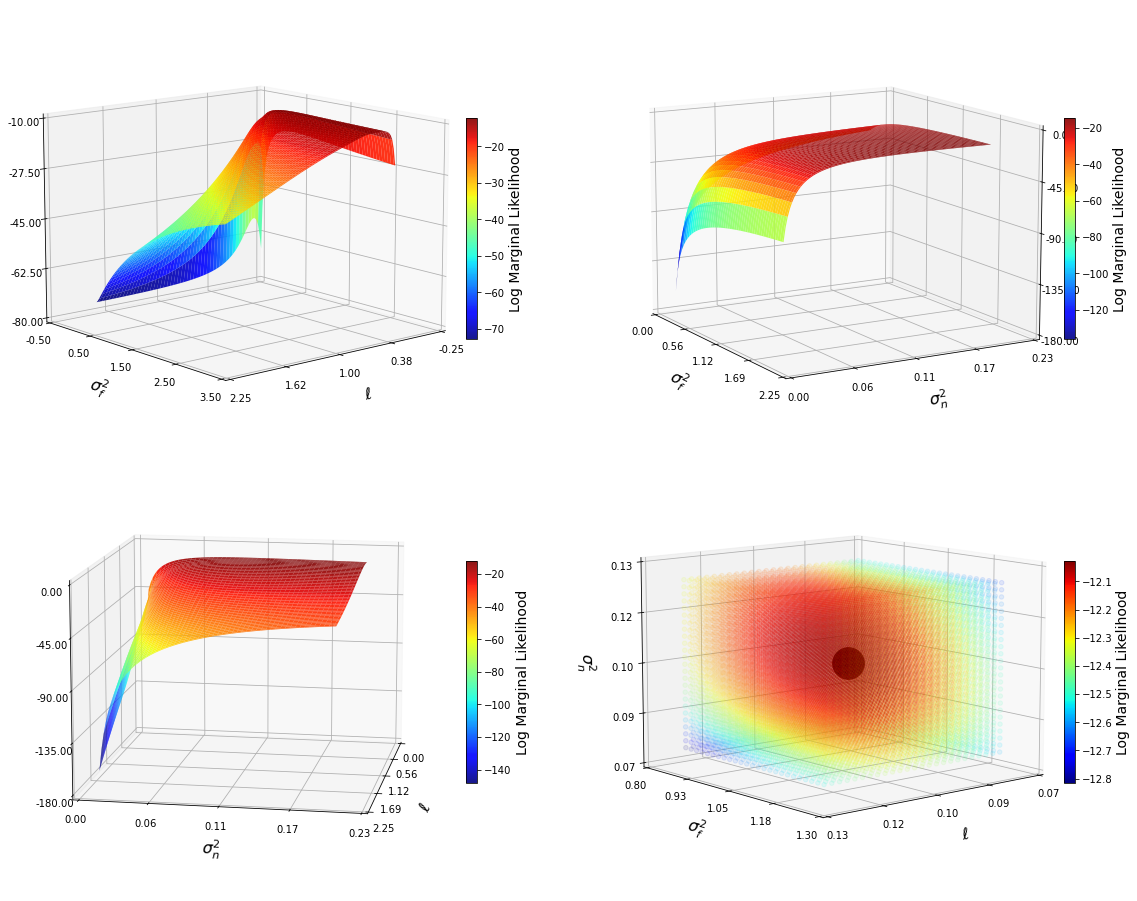
\includegraphics[width=0.8\textwidth]{LatexPlots/1dplots/LogLikeallparams.png}
    \caption[Visualising the log likelihood optimisation surfaces over the model parameters.]{For a GPR with noise where we have the noise as a hyperparameter we are forced to optimise a length \((\ell\)) hyperparameter, a variance \(\sigma_f^2\) hyperparameter and a noise \(\sigma_n^2\) hyperparameter. 
    Here we have kept one parameter constant on each graph and compared the log likelihood space varying the other two parameters. 
    In the upper left panel the noise is set to $\sigma^2_n= 0.1$, in the upper right panel the length is set at $ \ell=0.5$, in the lower left panel the variance is set at $\sigma^2_f=1.5$. 
    In the final panel we plot a 3-dimensional scatter plot and illustrate the point estimate given by the optimisation algorithm \texttt{"fmin\_l\_bfgs\_b"} as the black dot. This point is located at
    $(\sigma_f^2 = 1.16, \ell = 0.109 \sigma_n^2 = 0.105)$.}
   \label{fig:Optimising_Hyperparams}
\end{figure} 


\section{Quantifying Hyperparameter Uncertainty}
\label{sec: MCMC}
As shown in Figure~\ref{fig:Optimising_Hyperparams}, optimising hyperparameters does not necessarily yield a single “best” solution. 
Instead, there often exists a region of hyperparameter values that explain the data equally well, resulting in a flat or multi-modal log marginal likelihood surface.
Up to this point, the models considered have relied on point estimates (selecting the hyperparameters that maximise the log marginal likelihood and using them directly for prediction). 
While this process is convenient, by choosing one parameter we ignore the underlying uncertainty across hyperparameters that achieve similarly high likelihood scores. 
To account for this, we now aim to construct a posterior distribution over the hyperparameters, thereby enabling us to quantify and visualise uncertainty in their values.
%

We aim to build the posterior distribution over the hyperparameters \( \theta \), given the data \((X, y)\), this is expressed as:
%
\begin{equation}
p(\theta \mid y, X) = \frac{p(y \mid X, \theta) \, p(\theta)}{p(y \mid X)}
\end{equation}
where:
\begin{itemize}
    \item \( p(y \mid X, \theta) \) is the likelihood of the data given the hyperparameters,
    \item \( p(\theta) \) is the prior distribution over the hyperparameters,
    \item \( p(y \mid X) = \int p(y \mid X,\theta)p(\theta)d\theta \) is the marginal likelihood, serving as a normalising constant.
\end{itemize}
Since \( p(\mathbf{y} \mid X) \) is often intractable (unable to analytically intergate), we sample from the unnormalised posterior using MCMC sampling:
\begin{equation}
p(\theta \mid \mathbf{y}, X) \propto p(\mathbf{y} \mid X, \theta) \, p(\theta)
\end{equation}
%
We generate samples \( \{\theta^{(s)}\}_{s=1}^S \sim p(\theta \mid y, X) \) from this posterior distribution.
We build a distribution over the collection of these samples helping to visualise the uncertainty associated with each parameter. 
An example of this is done in figure~\ref{fig:MCMCresults}.
\begin{figure}[H]
    \centering
    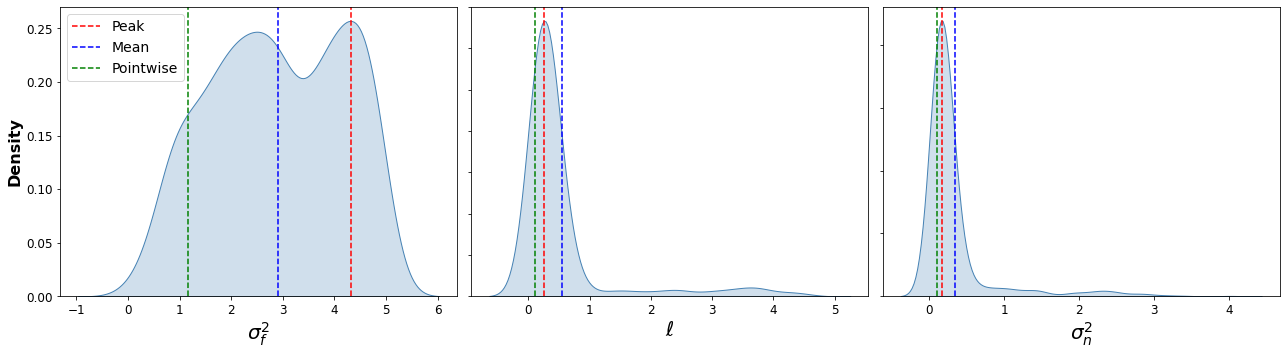
\includegraphics[width=\textwidth]{LatexPlots/1dplots/MCMCdistribution.png}
    \caption[Visualising the posterior distribution of the hyperparameters using MCMC.]{
    Results from an MCMC run using a Gaussian Process Regression model with an RBF kernel and a WhiteKernel to model noise. We used the point estimates from Figure~\ref{fig:Optimising_Hyperparams} as the starting point 
    for our samples. We sampled the parameter space using 12 walkers and taking 1000 steps with each walker. We discarded 100 of the initialed samples and thinned every 15 resulting in 720 final samples. 
    (For more details on this implementation refer to the Appendix \todo{MCMC appendix}.)
    Using these samples we plot the approximate posterior distributions for each hyperparameter. 
    the vertical red, blue and green lines indicate peak, mean, and pointwise estimates respectively.}
    \label{fig:MCMCresults}
\end{figure}
%

We observe in Figure~\ref{fig:MCMCresults} that the posterior for the signal variance hyperparameter \((\sigma_f^2)\) is nearly bimodal, with significant differences between the mean, mode, and point estimates. 
In these cases, relying on a single point estimate would lose critical information about model uncertainty.
To address this, we incorporate hyperparameter uncertainty directly into the predictive distribution by marginalising over the posterior \( p(\theta \mid y, X) \).
%
\begin{equation}
p(f_* \mid \mathbf{y}, X, X_*) = \int p(f_* \mid \mathbf{y}, X, X_*, \theta) \, p(\theta \mid \mathbf{y}, X) \, d\theta.
\end{equation}
Since this integral is also often intractable we approximate the marginalised predictive distribution using our MCMC samples \( \{\theta^{(s)}\}_{s=1}^S \):
%
\begin{equation}
p(f_* \mid \mathbf{y}, X, X_*) \approx \frac{1}{S} \sum_{s=1}^{S} p(f_* \mid \mathbf{y}, X, X_*, \theta^{(s)}).
\end{equation}
%
The resulting mean and variance are computed using the law of total variance:
%
\begin{equation}
\mathbf{E}[f_*] \approx \frac{1}{S} \sum_{s=1}^{S} \mu^{(s)}(f_*), \quad
\text{Var}[f_*] \approx \frac{1}{S} \sum_{s=1}^{S} \left[ \sigma^{2(s)}(f_*) + \left(\mu^{(s)}(f_*)\right)^2 \right] - \left( \mathbf{E}[f_*] \right)^2.
\end{equation}
This procedure allows the final predictive distribution to reflect both data noise and model uncertainty.


\section{Multi-Dimensional GPR}
\label{sec:multidims}
\todo{Improve or link better}
To model functions with multiple input dimensions, a common approach is to construct kernels that operate over each input dimension individually
and then combine them by multiply them [\cite{bible},\cite{gprthesis}]. For example, multiplying RBF kernels defined on each input dimension yields a multi-dimensional RBF kernel.
A specific case of this is the RBF-ARD (Automatic Relevance Determination) kernel, which assigns a separate lengthscale parameter \( \ell_d \) to each input dimension \( d \). Since an RBF ultilises an exponential function
the product of the kernel can be written as the exponential of the sum of the different dimension. Figure~\ref{fig:2dkernels} shows how different kernels with different length-scales can combine to produce a kernel in higher dimensions.
\begin{equation}
    k(\mathbf{x}, \mathbf{x}') 
    = \sigma_f^2 \prod_{d=1}^D \exp\left( -\frac{1}{2} \frac{(x_d - x_d')^2}{\ell_d^2} \right)
    = \sigma_f^2 \exp\left( -\frac{1}{2} \sum_{d=1}^D \frac{(x_d - x_d')^2}{\ell_d^2} \right)
\end{equation}
    

\begin{figure}[H]
    \centering
    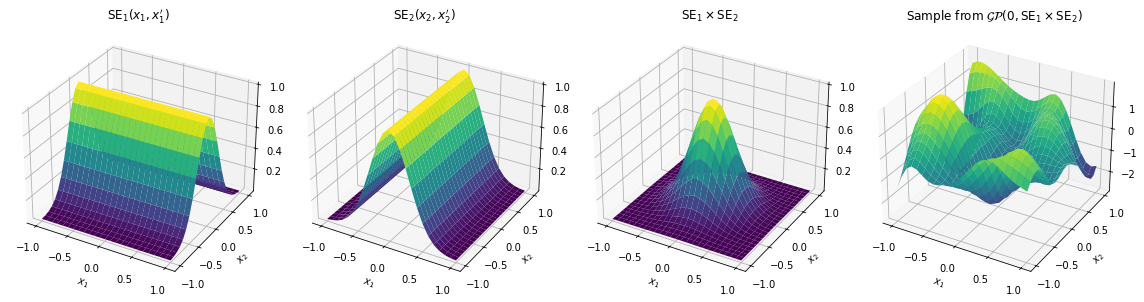
\includegraphics[width=\textwidth]{LatexPlots/final_gps_plots/2dkernels.png}
    \caption[Visualising the construction of a multi-dimensional kernel.]{
    Visualisation of constructing a two-dimensional kernel by multiplying two one-dimensional RBF kernels, each operating on a separate input dimension. Both kernels use a length scale of \(\ell = 0.3\). 
    The resulting product kernel models smooth interactions across both dimensions, and a sample drawn from the corresponding GP prior is shown.}
    \label{fig:2dkernels}
\end{figure}

\chapter{Methods}
\begin{figure}[H]
    \centering
   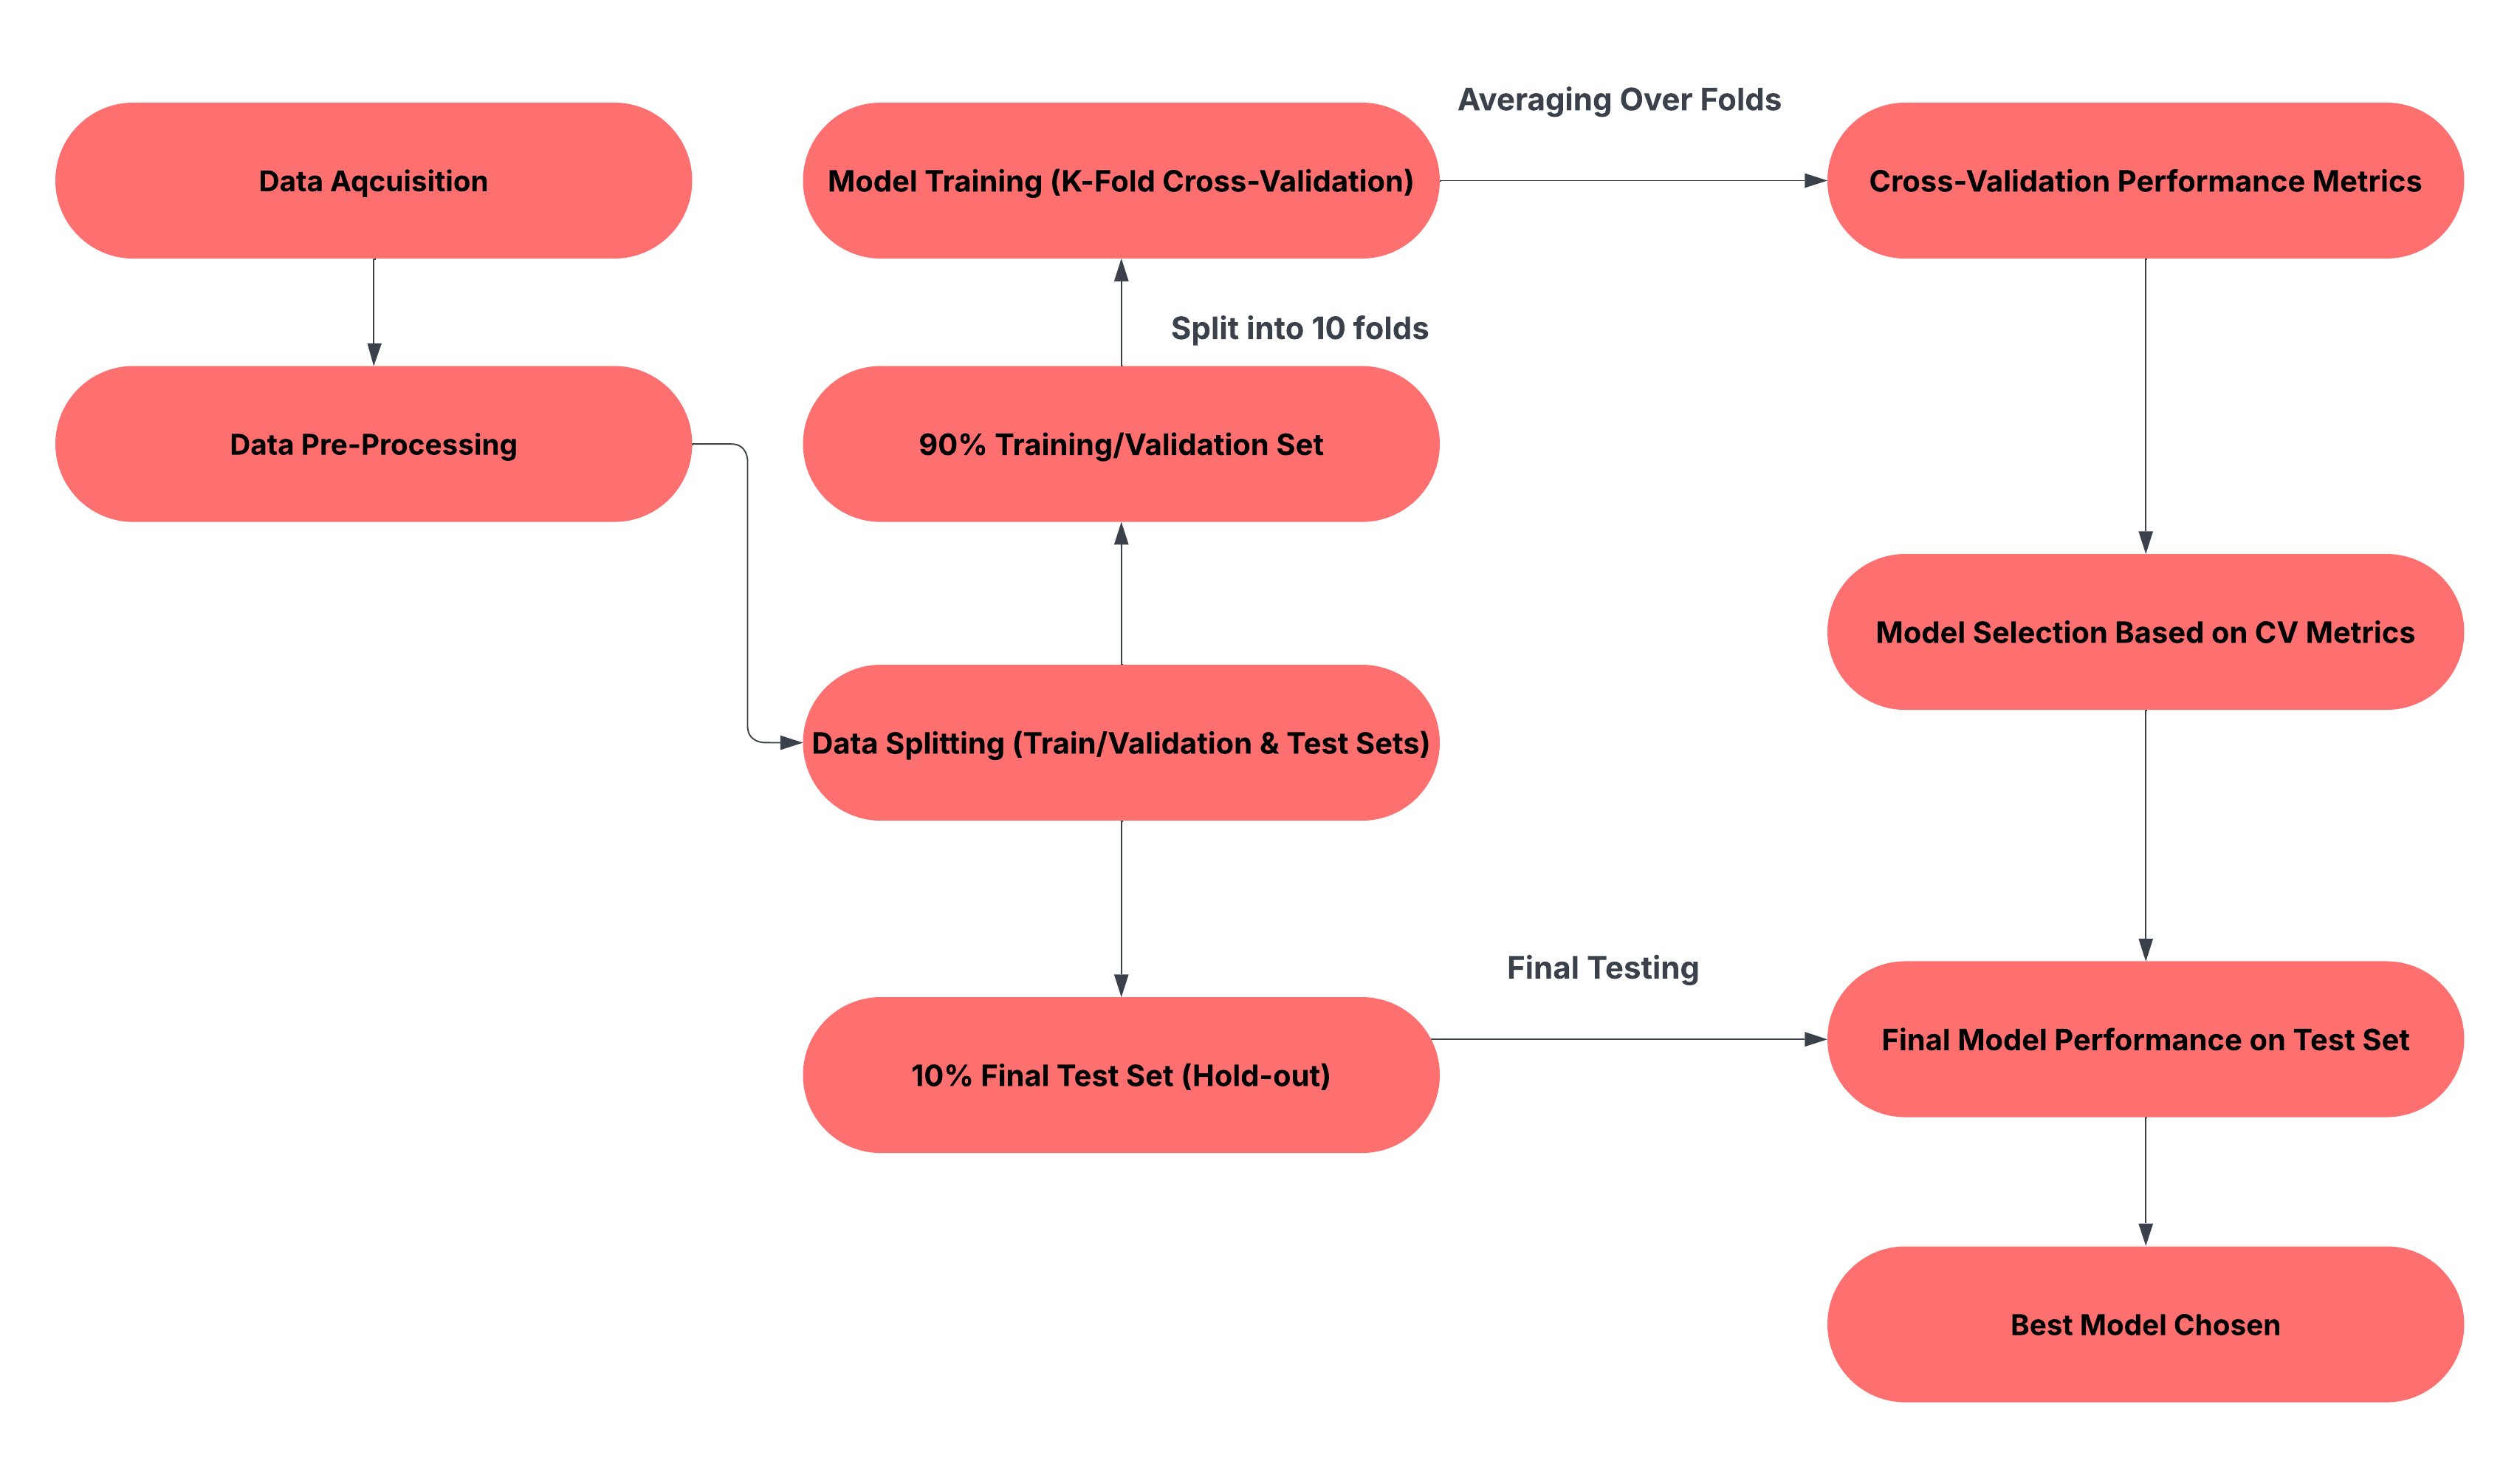
\includegraphics[width=0.8\textwidth]{LatexPlots/Flowchart.png}
    \caption[Flow chart of the process taken from data processing to selecting the best performing model.]{
        This flowchart provides a highlevel summarry of the methodology. Starting from data acquisition and preprocessing, 
        through k-fold cross-validation for model training and evaluation, 
        to the selection of the best performing model based on test set results. All of which is explained in detail below.}
    \label{fig:flowchart}
\end{figure}
\section{The Models}
\label{subsec:Models}
To build a robust Gaussian Process Regression (GPR) model, I constructed a comprehensive set of model configurations by combining the kernels described in Section~\ref{sec: Kernels} with the noise-handling techniques introduced in Section~\ref{sec: Handlingnoise}. 
A full summary of models implemented is provided in Table~\ref{tab:model_summary}. Below, we outline the different classes of models explored:

\noindent
\subsection{Homoscedastic Noise Models}
\begin{itemize}
    \item \textbf{White Kernel:} Noise is modelled as a global hyperparameter using the \texttt{WhiteKernel} class added to each kernel.
    After initial examination I found that the results of optimising the noise hyperparameter varied massively with the noise bounds. 
    To better understand how each model varied with noise hyper-paraters I implemented three variants with different noise bounds:
    \begin{itemize}
        \item \texttt{whitenoerror}: loose bounds \((10^{-6}, 10^6)\),
        \item \texttt{whiteminmaxerror}: bounds set using the 5th and 95th percentiles of the known standard deviations,
        \item \texttt{whitemeanerror}: bounds centered around the mean known uncertainty.
    \end{itemize}
\end{itemize}
%
%

\subsection{Heteroscedastic Noise Models}
\begin{itemize}
    \item \textbf{Known Noise:} The \texttt{fixedalpha} model assumes noise variance is known at each input and adds this directly into the kernel diagonal using the \texttt{alpha} argument of \texttt{GaussianProcessRegressor}.
    \item \textbf{Monte Carlo Sampling:} The \texttt{montecarlo} model accounts for our observed mismatch values having noise associated with them. It adds noise to our observations and builds posterior distributions for each of these ''noisy'' samples. 
    \item \textbf{Additive Kernel Structures:} The \texttt{combinekernel} models use additive combinations of kernels to capture both smooth and variable structures in the mismatch data. From our examination of the kernels in Section~\ref{sec: Kernels} we have seen that the RBF producs smooth curves while kernels like the Matern, Rational Quadratic and the Laplace produce more variational fits.
            From Examining our data in Section~\ref{sec:data_description} we noticed smooth general shapes with local variations. This was the motivation to make an additive Kernel of the form 
    \begin{equation}
        k(x, x') = \sigma_{f,1}^2k_{\mathrm{RBF}}(x, x') + \sigma_{f,2}^2k_{\mathrm{extra}}(x, x'),
    \end{equation}
    where \(k_{\mathrm{extra}}\) is one of Matern, RationalQuadratic, or Laplacian. We constrain the RBF Kernel to large \(\ell\) parameters with an optimisation range of \((0.5,100)\) since this will force the RBF Kernel to model the general smooth shape over inputs
    and then we give the additional kernel much smaller \(\ell\) bounds so that it captures the local variation. \(\sigma_{f,1}^2\) and \(\sigma_{f,2}^2\) are the signal variance for each kernel and capture the weighting of each model towards this combined signal variance.
\end{itemize}
%
%

\noindent
\subsection{Hybrid Model}
\begin{itemize}
    \item \textbf{Hybrid Noise:} The \texttt{hybrid} model includes both fixed known noise and a trainable noise parameter. The fixed component helps get accurate levels of uncertainty where the noise is known (training inputs), while the learnable part generalizes to unseen regions.
\end{itemize}
%
For each configuration, the kernel hyperparameters were optimised by maximising the log marginal likelihood, as described in Section~\ref{sec: Hyper_parameters}. 
Specific implimentation details are available in Section~\ref{subsubsec:implementdetails}
%
%
%

\begin{table}[h!]
    \renewcommand{\arraystretch}{1.3}
    \centering
    {\fontsize{8}{9.5}\selectfont
    \begin{tabular}{|l|l|l|l|}
    \hline
    \textbf{Model Label} & \textbf{Noise Type} & \textbf{Noise Optimisation Bounds} & \textbf{Kernels} \\
    \hline
    \texttt{whitenoerror} & Homoscedastic & \((10^{-6}, 10^6)\) & All kernels \\
    \texttt{whiteminmaxerror} & Homoscedastic & 5\% lower and 95\% upper error & All kernels \\
    \texttt{whitemeanerror} & Homoscedastic & \((0.7\mu_{\text{error}}, 1.3\mu_{\text{error}})\) & All kernels \\
    \hline
    \texttt{fixedalpha} & Heteroscedastic & -- & All kernels \\
    \texttt{montecarlo} & Heteroscedastic & Sampling & All kernels \\
    \texttt{combinekernel} & Heteroscedastic & -- & RBF + Matern \\
    \texttt{combinekernel} & Heteroscedastic & -- & RBF + RationalQuadratic \\
    \texttt{combinekernel} & Heteroscedastic & -- & RBF + Laplace \\
    \hline
    \texttt{hybrid} & Hybrid & \((10^{-6}, 10^6)\) & All kernels \\
    \hline
    \end{tabular}}
    \caption[Listing model variations used in cross validation runs.]{Summary of the Gaussian Process Regression models evaluated.
     ''All kernels'' refers to the RBF, Matern, Rational Quadratic, ExpSine Squared and the Laplace kernels discussed in Section~\ref{sec: Kernels}. In the ''All Kernels'' case the method 
     was ran for every kernel.}
    \label{tab:model_summary}
\end{table}

\subsection{Model Evaluation Metrics}
\label{sec:metrics}
To assess the performance of each GPR model, I used six evaluation metrics. These metrics were discussed and chosen in \cite{metrics} for the 
specific reason that they offer robust metrics that capture different information about the model. 
In this paper they divide the metrics into two types Average Expected Error \textbf{AEE} metrics and correlation metrics. 

\subsection{AEE Metrics}
\begin{itemize}
    \item \textbf{Root Mean Squared Error (RMSE)} \( \left(\sqrt{\frac{1}{N} \sum (y_i - \hat{y}_i)^2} \right)\): Measures the average distance between true values and the prediction. Since at each point the error is squared the RMSE has a heavier penalty for larger errors.
    \item \textbf{Mean Absolute Error (MAE)} \( \left( \frac{1}{N} \sum |y_i - \hat{y}_i|\right) \):  The MAE measures the average absolute difference between predicted and true values. It is less sensitive to larger errors than the RMSE since it is not quadratically scaled.
    \item \textbf{Figure of Merit (FOM)} \( \left( \frac{\text{RMSE}}{\sigma}\right) \): This is the ratio of our RMSE to the standard deviation. It can be interpreted as the average expected error scaled by the spread of the data. 
    Lower FOM values indicate higher model accuracy, as they imply that the model's predictive error is small compared to the variation in the data. A value near zero reflects excellent predictive performance, while larger values suggest less accurate predictions.
\end{itemize}

\subsection{Correlation Metrics}
\begin{itemize}
    \item \textbf{Coefficient of Determination}\(\left(\mathbf{R^2}\right)\)\( \left(1 - \frac{\sum (y_i - \hat{y}_i)^2}{\sum (y_i - \bar{y})^2}\right) \): Finds 1 - the ratio of how well the mean predicts the true values compared to the model predictions. Measures how much better our model is at predicting than a baseline mean prediction.
    
    \item \textbf{Adjusted} \(\mathbf{R^2 \left( \bar{R^2}\right)}\)\( \left( 1 - (1 - R^2) \cdot \frac{n - 1}{n - p - 1} \right) \): Updates our \( R^2 \) value to take account the number of predictors compared to the number of observed points. This helps to prevent over-fitting because trivially if we used \(p=n\) predictors we should get perfect results but our model would be drastically over-fitted.
    
    \item \textbf{Pearson Correlation Coefficient}\( \left(\frac{\text{cov}(y, \hat{y})}{\sigma_y \sigma_{\hat{y}}} \right) \):  Quantifies the linear relationship between true and predicted values.
\end{itemize}
In \cite{metrics} the author concluded that lower AEE metrics (close to 0) correspond to higher regressor accuracy, and higher correlation metrics (closer to 1) correspond to better predictions. We set out to evaluate our models with these metrics.

\section{Model Training, Testing and Comparisons}
%
%
\subsection{Cross Validation on all Model Types}
To ensure that each of the models was not overly dependent on a particular dataset and to mitigate overfitting, 
k-fold cross-validation was implemented, and the metrics outlined in Section~\ref{sec:metrics} were evaluated on each validation fold. 
This approach is supported by Rasmussen and Williams in \cite[Ch.~5]{bible}, where cross-validation is discussed as a method for model selection.
The full dataset was divided into a 90--10 split, where 90\% of the data was used for 10-fold cross-validation, and the remaining 10\% was held out 
as an untouched test set for final evaluation. During cross-validation, each model was trained on 9 out of the 10 folds and evaluated on the remaining fold, 
with the process being repeated such that every fold served as the validation set once. For each fold, model predictions were compared against the true values using the six metrics
described in Section~\ref{sec:metrics}.
To analyse model stability and consistency, the distribution of each metric across folds was visualised using box plots for each model type. Additionally, the mean performance for every metric 
across all folds and model types was plotted.

Each model was then ranked in comparison to all other models for each individual metric (lower is better for AEE, higher is better for correlation) receiving a score from \(1\) (best in that metric)
to \(33\) (worst performing model for that metric), and these rankings were averaged across all metrics to produce an overall ranking table based on each models average ranking.
The overall ranking of every model was plotted as a heat-map to allow easier interpretation
of how rankings varied.To understand relationships between metrics, a dendrogram was constructed based on the correlation of each metrics model rankings, 
enabling the identification of clusters of similar metrics and those with differing behaviours. 
Finally, to ensure robust generalisation, the most distinct metrics identified from the dendrogram were used to 
create a scatter plot comparing model performance, and a subset of models that consistently performed best across these dimensions were selected.

 \subsection{Final Testing}
In the final stage, each of the shortlisted models was retrained on the full 90\% cross-validation training set and evaluated on the held-out 10\% test set. Model predictions were compared to the true values using the same six metrics, and performance was visualised to identify the most accurate and robust candidates.
The best over-all model was selected at this stage. Markov Chain Monte Carlo (MCMC) (explained in Section~\ref{sec: MCMC}) was performed on this model
to construct posterior distributions over its hyperparameters, allowing for a visual and probabilistic assessment of hyperparameter uncertainty. 
The final model posterior distribution was then marginalised over its hyperparameters and was
compared against the pointwise posterior using performance matrics and plotting both posteriors at cross-cuts of the data.
 

\subsection{Implementation Details}
\label{subsubsec:implementdetails}
All models were implemented in Python. Gaussian Process Regression was carried out using the \\
\texttt{GaussianProcessRegressor} class from the \texttt{scikit-learn} library, with hyperparameter optimisation performed using the 
default \texttt{optimizer="fmin\_l\_bfgs\_b"} routine. 
For MCMC sampling, I used the \texttt{emcee} package. Interpolation was performed using \texttt{scipy.interpolate}. 
To ensure reproducibility, I consistently set the random seed to 42 throughout all experiments. All code is available at \cite{githubrepo}.
%
%
%
\chapter{Results}
\section{Cross-Validation Performance}
The cross validation results for all model types discussed in Section~\ref{subsec:Models} are visualised in Figure~\ref{fig:broad_comparison}. A few notable observations emerge. Firstly, the \texttt{montecarlo} noise modeling method performs poorly.
This may be due to the fact that the noise associated with our data is relatively large. When sampling different noise levels, this results in a mixture of large- and small-noise systems whose effects, when averaged, tend to cancel out—leading to overly generalised predictions.
We also find that interestingly incorporating the true noise in our GP results in worse performance than learning the noise as a hyperparameter.
This is evident by the relatively poor results from \texttt{fixedalpha}, and the slightly improved, but still limited, performance of \texttt{hybrid}.
We conclude that learning the noise via a hyperparameter is the most effective approach for our models.
\begin{figure}[H]
    \centering
    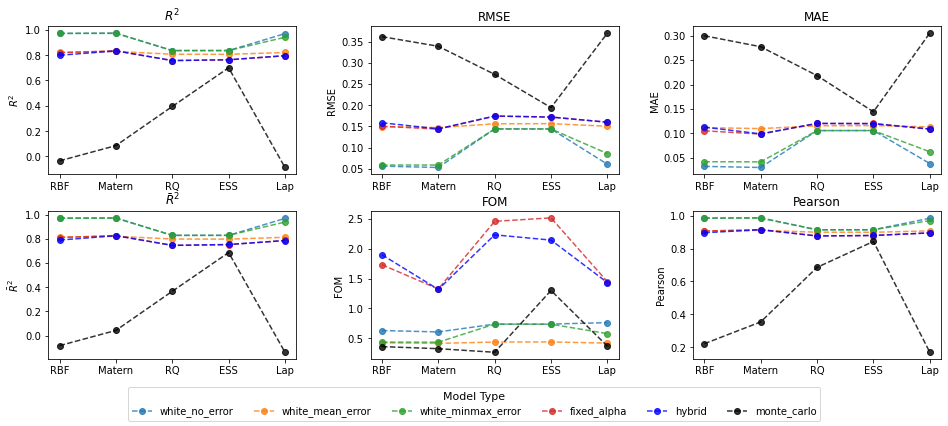
\includegraphics[width=\textwidth]{LatexPlots/CV_plots/metrics_compared.png}
    \caption[Comparing average metrics over all cross validation folds between all model types.]{Comparison of the average performance of each model type and for each kernel across all 10 folds of the training/validation data for each metric. Note: The \texttt{combinedkernel} approach is excluded here for clarity, but is included in all subsequent evaluations.}
    \label{fig:broad_comparison}
\end{figure}
The average rank of each model across all metrics is presented in Table~\ref{tab:rankingtable} and all the plots in Figure~\ref{fig:CV_sidebyside} label the models as their final ranking in this table.
The heatmap in Figure~\ref{fig:CV_sidebyside} (left) illustrates the rankings by metric, showing that most rankings are fairly consistent. To explore this further, a dendrogram of pairwise distances based on the correlation of metric rankings is plotted in Figure~\ref{fig:CV_sidebyside} (middle).
The dendrogram highlights three clusters of metrics with different ranking behaviors: the first cluster (including \(R^2\), adjusted \(R^2\), RMSE, and Pearson) ranks models similarly, while the MAE rankings differ slightly, 
and the FOM rankings vary significantly. This pattern is also evident in the heatmap, where FOM colors stand out from the other metrics.
To select a model that generalizes well across all metrics, we compare models using one metric from each cluster: \(R^2\) (from cluster 1), MAE, and FOM. 
In Figure~\ref{fig:CV_sidebyside}(right), we visualize model performance across these metrics. This visualization clearly identifies a top group of eight models, forming an optimal cluster, which is examined in more detail in the following section.
\begin{figure}[H]
    \centering
    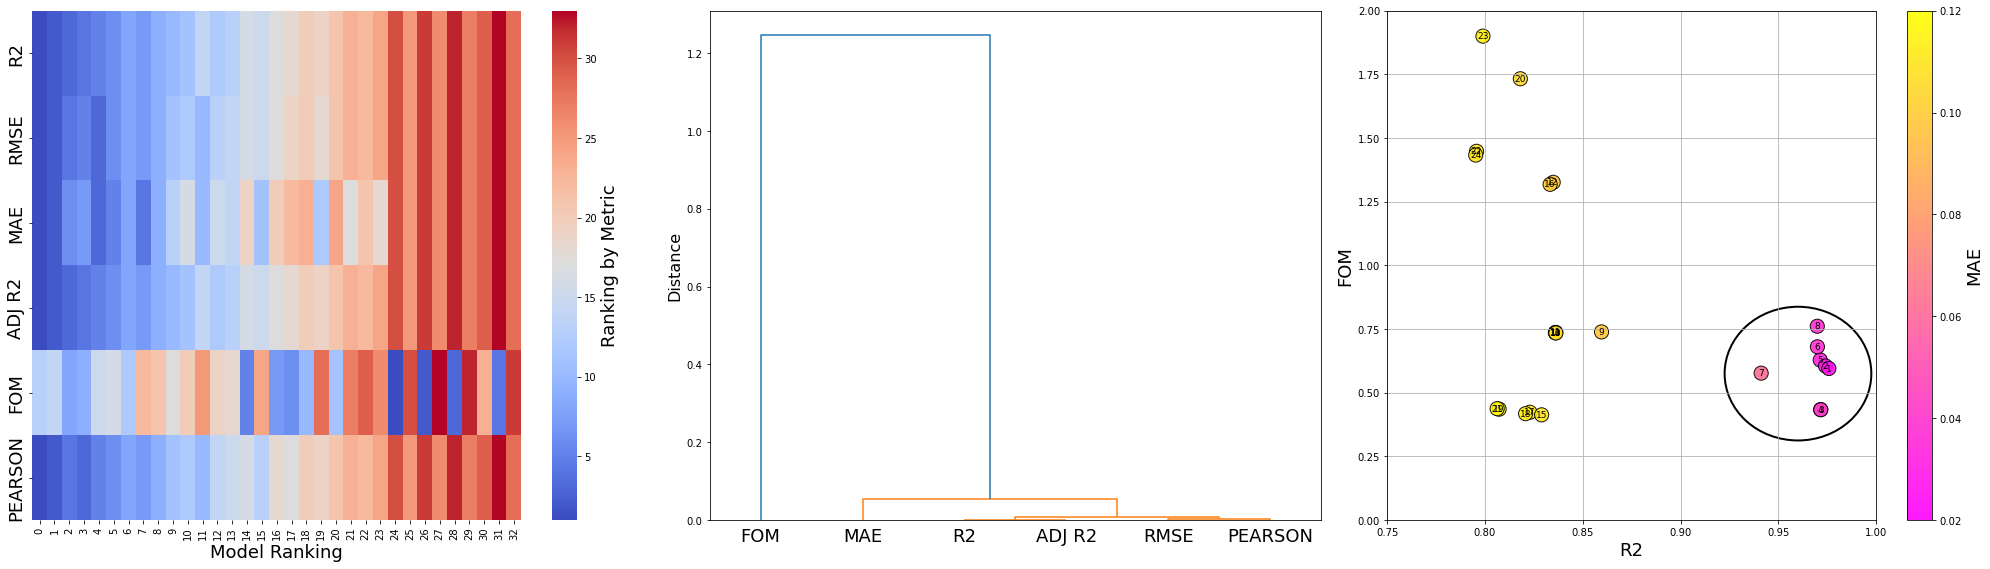
\includegraphics[width=\textwidth]{LatexPlots/CV_plots/ranking_visualisation.png}
    \caption[Visualising the ranking of each model after cross validation.]{Left: Heatmap showing each model’s rank across the evaluation metrics. The x-axis lists models according to their ranking in Table~\ref{tab:rankingtable}, and the y-axis shows the metrics. The color bar represents rank (blue indicates better rank, red indicates worse). 
    Middle: Dendrogram showing hierarchical clustering of metrics based on how similarly they rank models. The vertical axis denotes correlation distance—smaller values indicate higher agreement between metric rankings.
    Right: Scatter plot of all models with \(R^2\) on the x-axis, FOM on the y-axis, and MAE represented by the color of each point. Models are indexed by their rank from Table~\ref{tab:rankingtable}.}
    \label{fig:CV_sidebyside}
\end{figure}



\section{Training on 90\% of Data}
After identifying the top 8 models forming a high-performing cluster in Figure~\ref{fig:CV_sidebyside} (right),
we retrained these models using the full 90\% of the data previously used for cross-validation. The optimized hyperparameters for these final models are detailed in Table~\ref{tab:final_gpr_hyperparams}. 
To evaluate performance, we tested each model on the remaining 10\% of unseen data and visualized their results in Figure~\ref{fig:comparing_metrics}.
From the heatmap we can see that the rankings remain fairly consistent across metrics, with some variation in the FoM. The best performing models on the test set seperate themselves in the scatter plot. The best 3 models have high \(R^2 \sim 0.99\) , low FOM \(\sim 0.45\) and low MAE \(\sim 0.04\).
From Table~\ref{tab:finalmadelsrankingtable} we can see that these top 3 models correspond to the \texttt{RBFMat}, \texttt{Matnoerr} and \texttt{RBFnoerr}.
\begin{figure}[H]
    \centering
    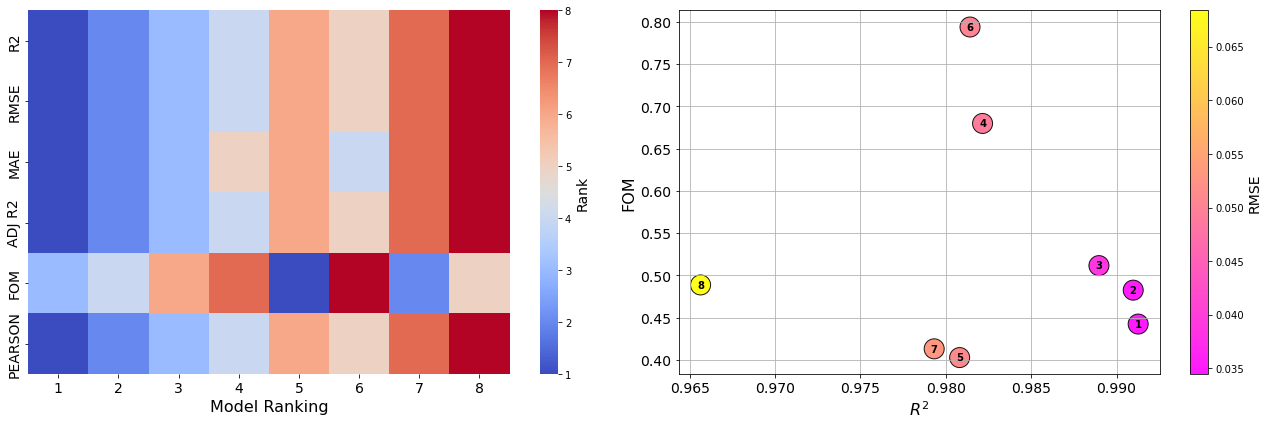
\includegraphics[width=\textwidth]{LatexPlots/final_gps_plots/metric_of_finalists_comparison.png}
    \caption[Visualising the ranking of each model on the test data.]{Left: Heatmap of top 8 model rankings by metric indexed by ranking.
    Right: Scatter of FOM against \(R^2\) with the colour bar representing the RMSE.
    The Rankings are given in Table~\ref{tab:finalmadelsrankingtable}.}
    \label{fig:comparing_metrics}
\end{figure}
\todo{reword interpretation, review at least}
Plotting the top 8 model predictions for various cross-cuts in Figure~\ref{fig:crosscuts_bestmodels}, we observe that while all models perform well, they differ in how they handle local noise.
The \texttt{RBFMat} model remains smooth in regions with sparse data and then responds sharply in regions containing outliers or local irregularities.
This behaviour is reflected in its optimized hyperparameters (Table~\ref{tab:final_gpr_hyperparams}). The RBF component has long characteristic length scales (around 1.0--1.5) and a large scale factor ($2.34$),
which captures the global smooth structure of the data. Meanwhile, the Matern component has much shorter length scales (mostly $< 0.5$) and a smaller scale ($0.207$), allowing it to respond to local variability—effectively modeling input-dependent noise.
Examining models that use a single kernel and a constant noise hyperparameter we see that the optimised noise hyperparameter is very small with \(\sigma_n^2 \ll 0.01\). For the models with tighter noise bounds (\texttt{minmaxerr})the optimiser always opts for the same lower noise bound. The loser bound models (\texttt{noerr})
also results in small noise hyperparameter values. This suggests that the GP is compensating for noise directly through the kernel, not through the explicit noise model. This provides further credibility to the \texttt{RBFMat} combined model, where the noise appears to be effectively captured within the Matern kernel.
Finally, examining Laplacian-based kernel models (\texttt{Laplace\_noerr} and \texttt{Laplace\_minmaxerr}), which only have a single hyperparameter ($\gamma$), they still perform reasonably well but tend to produce more linear predictions. This is likely due to their limited flexibility compared to other kernels.
Based on our metrics calculated and visualised in Figure~\ref{fig:comparing_metrics} and our qualitative examination of the crosscuts in Figure~\ref{fig:crosscuts_bestmodels}, we see that the \texttt{RBFMat} model offers the best trade-off between flexibility, interpretability, and robustness.
%
\begin{figure}[H]
    \centering
    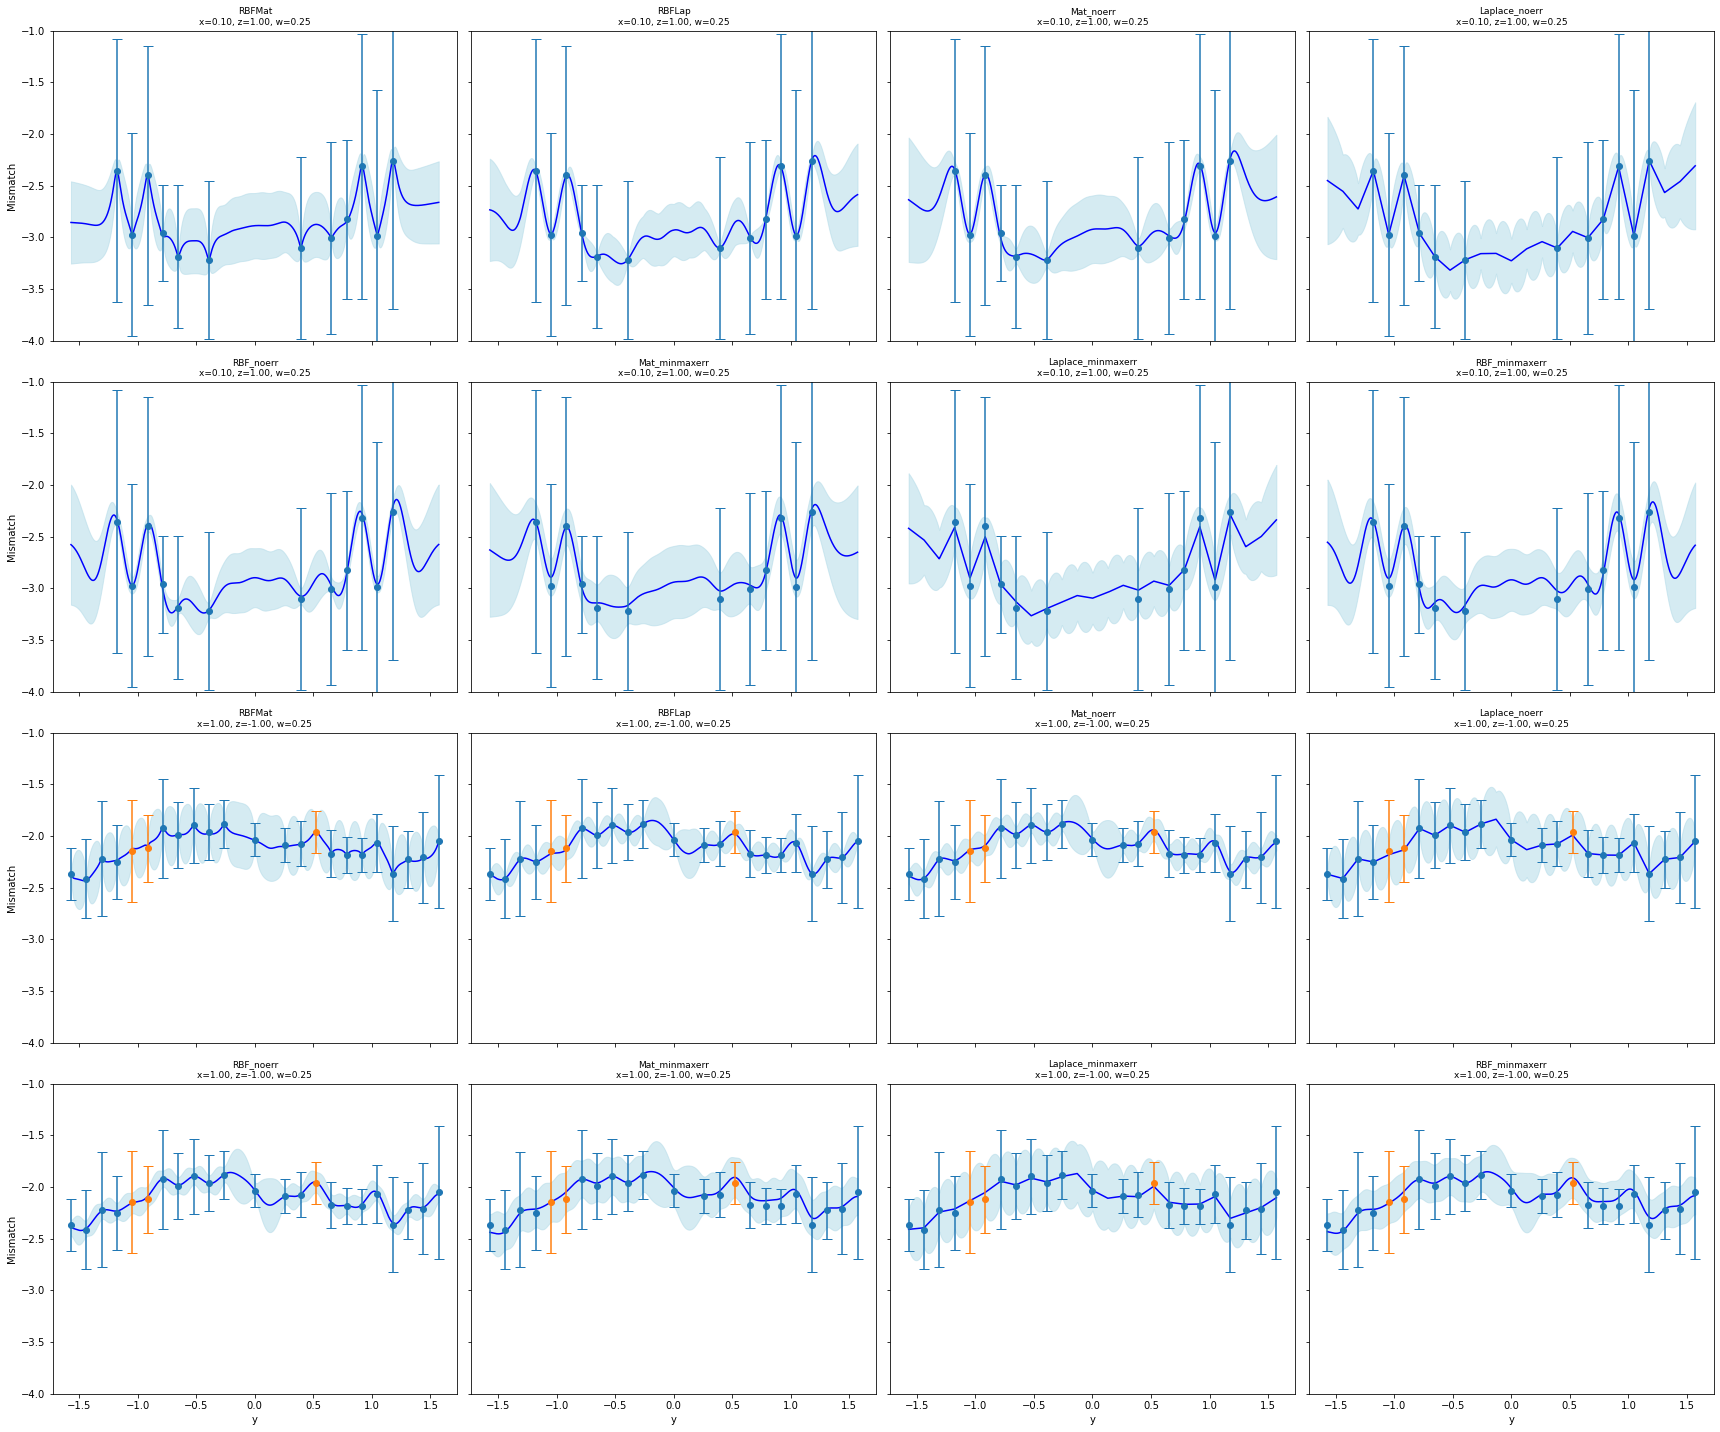
\includegraphics[width=1\textwidth]{LatexPlots/final_gps_plots/gps_crosscuts_bestmodels.png}
    \caption[Comparing Cross-cuts of best 8 models.]{Comparing Cross-cuts of best 8 models. Each models hyperparameters can be found in Table~\ref{tab:final_gpr_hyperparams}. 
    Recall that $z=1\ (z=-1)$ corresponds to mass ratio of $q=1\ (q=1/4)$, and similarly $w=0.25$ corresponds to $M_\text{tot}=37.5M_\odot$. The blue shaded region indicates the 95\% credible region for each model
    and the blue line is posterior mean. Blue scatter points represent training inputs and orange are test points.\todo{Reference futher graphs in appendix},
    \todo{Add 2d visuals aswell}}
    \label{fig:crosscuts_bestmodels}
\end{figure}

\begin{table}[H]
\centering
\footnotesize  % Smaller than normalsize, slightly larger than scriptsize
\renewcommand{\arraystretch}{1.15}  % Slightly tighter row spacing
\setlength{\tabcolsep}{4pt}  % Reduce column padding
{\fontsize{7}{8.5}\selectfont
\begin{tabular}{|c|c|c|c|c|c|c|}
\hline
\textbf{Model} & \textbf{Kernel 1} & $\mathbf{\sigma_{f,1}^2}$ & \textbf{Length Scales 1} & \textbf{Kernel 2} & $\mathbf{\sigma_{f,2}^2}$ & \textbf{Length Scales 2 / Noise} \\
\hline
\texttt{RBFMat} & RBF & $2.34$ & $[1.00, 1.51, 1.38, 1.36]$ & Mat ($\nu = 0.75$) & $0.207$ & $[0.0996, 0.0582, 0.414, 2.31]$ \\
\texttt{RBFLap} & RBF & $0.354$ & $[0.10, 0.10, 1.18, 2.91]$ & Lap ($\gamma = 0.964$) & $0.292$ & --- \\
\texttt{Mat\_noerr} & Mat ($\nu = 1.75$) & $0.926$ & $[0.227, 0.20, 1.15, 2.85]$ & White & --- & $\sigma_n^2 = 0.00637$ \\
\texttt{Laplace\_noerr} & Lap ($\gamma = 0.358$) & $7.24$ & --- & White & --- & $\sigma_n^2 = 10^{-6}$ \\
\texttt{RBF\_noerr} & RBF & $0.728$ & $[0.112, 0.112, 0.958, 1.6]$ & White & --- & $\sigma_n^2 = 0.00728$ \\
\texttt{Mat\_minmaxerr} & Mat ($\nu = 1.75$) & $1.14$ & $[0.27, 0.22, 1.34, 4.73]$ & White & --- & $\sigma_n^2 = 0.0439$ \\
\texttt{Laplace\_minmaxerr} & Lap ($\gamma = 0.284$) & $6.60$ & --- & White & --- & $\sigma_n^2 = 0.0439$ \\
\texttt{RBF\_minmaxerr} & RBF & $0.821$ & $[0.12, 0.115, 1.19, 2.52]$ & White & --- & $\sigma_n^2 = 0.0439$ \\
\hline
\end{tabular}}
\caption[The optimized hyperparameters for the final 8 GPR models.]{This table contains the optimized hyperparameters for the final 8 GPR models. $\sigma_{f,1}^2$ and $\sigma_{f,2}^2$ represent the constant factor the each kernel is multiplied by and is referred to as the signal variance since it controls the amplitute of the resulting model.
The Length scales are the corresponding length scales for each dimension and then $\sigma_n^2$ is the optimised noise hyperparameter introduced by the \textsc{WhiteKernel}. Mat and Lap refer to the Matern and Laplacian kernel.}
\label{tab:final_gpr_hyperparams}
\end{table}

\section{Hyperparameter Uncertainty}
We construct the posterior distribution over the \texttt{RBFMatern} model's hyperparameters using MCMC sampling. As shown in Figure~\ref{fig:MCMCRBFMatern}, it is evident that the RBF kernel is capturing the long length scale smooth variations in the data. This is evident since the RBF length span larger \(\ell\) values than those of the Matern kernel posterior.
Furthering examining the distributions, we find that some parameters - such as \((\sigma_{f,2}^2, \ell_5,\ell_1)\)- have sharply peaked distributions with low variance,indicating relatively low uncertainty in their posterior distribution. 
In contrast parameters such as \(\sigma_{f,1}^2 , \ell_8\) exhibit nearly bi-model distributions with large variance, demonstrating that these regions of the hyperparameter space are highly uncertain.

This uncertainty in \(\sigma_{f,1}^2\) can be understood by examining the underlying data. While the true data often exhibits global smooth trends, there are regions where it becomes noisy and has abrupt variations. As a result, 
the optimiser appears to struggle between assigning a higher or lower weight to the RBF kernel relative to the Matern kernel. 
A higher weight favours the RBF component which would emphasise global smoothness, whereas a lower weight allows the Matern kernel to account for local fluctuations. 
Ultimately, the optimiser resolves this ambiguity by selecting a compromise between the two competing modes by choosing the 
mean of the distribution.

\begin{figure}[H]
    \centering
    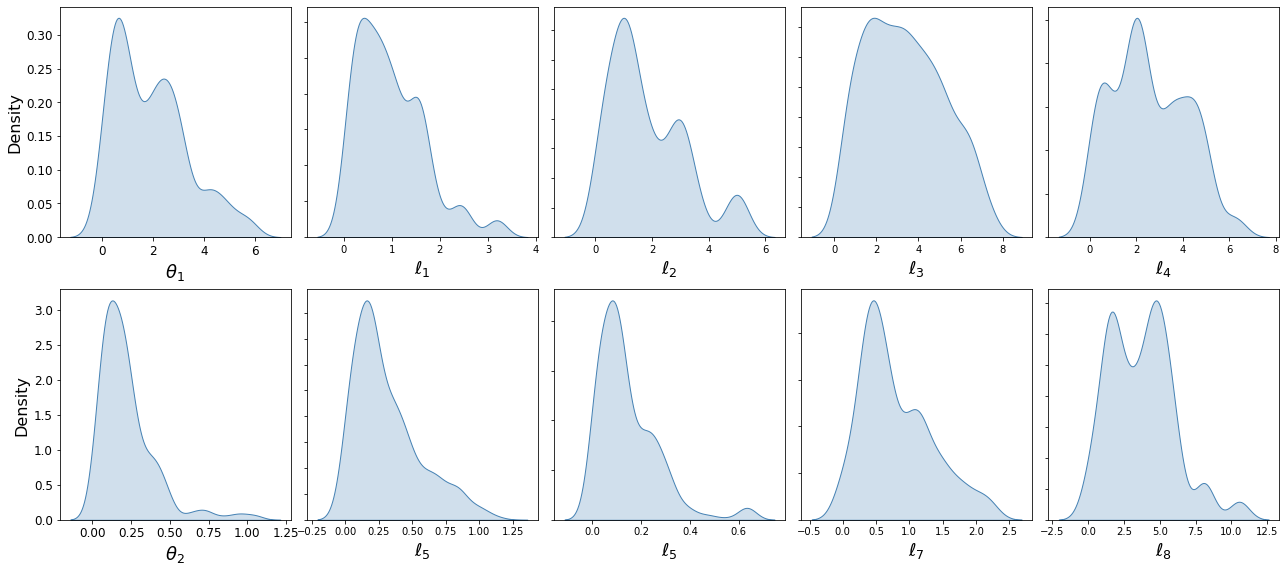
\includegraphics[width=1\textwidth]{LatexPlots/final_gps_plots/MCMCRBFMat.png}
    \caption[The hyperparameter posterior of the best \texttt{RBFMatern} model.]{The hyperparameter posterior of the best \texttt{RBFMatern} model. The model hyperparameters from Table~\ref{tab:final_gpr_hyperparams} initialise each of the walkers (4 walkers for every extra parameter so 40 walkers). For each walker we generate 300 samples and use a burnin of 100 and a thin of 15 resulting in a total of 560 samples used to build this distribution.
    The resulting parameter distributions are plotted. The vertical red, blue and green lines indicate peak, mean, and pointwise estimates respectively.}
    \label{fig:MCMCRBFMatern}
\end{figure}
To visualise how the parameter uncertainty effects the final posterior predictive distribution, we marginalise over our sampled hyperparameter posteriors and compare this prediction to the previous pointwise results of the \texttt{RBFMatern} model shown in Figure~\ref{fig:crosscuts_bestmodels}.
Figure~\ref{fig:MCMCvsmarginalised} reveals that the marginalised MCMC credible intervals are noticeably wider than those of the pointwise model, especially in regions with sparse or noisy data. This is expected since the marginalised model is taking extra hyperparameter
uncertainty into account. 
%
\begin{figure}[H]
    \centering
    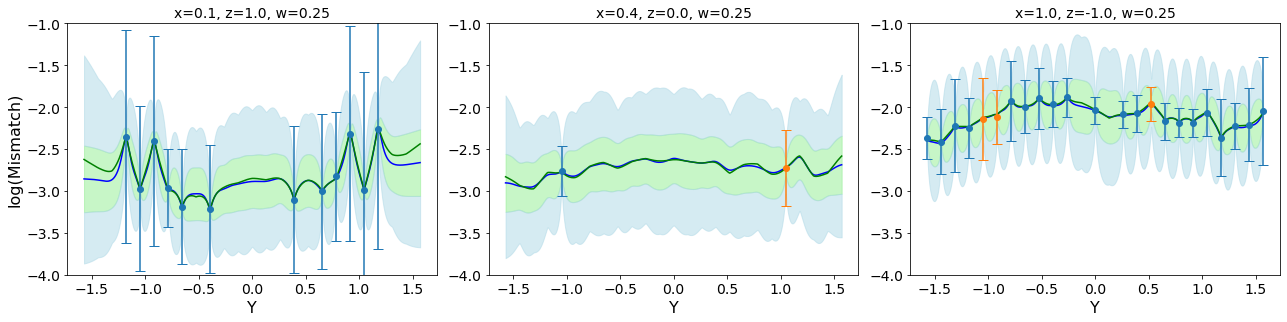
\includegraphics[width=1\textwidth]{LatexPlots/final_gps_plots/MCMCpointwisecomparison_all.png}
    \caption[Comparing the pointwise \text{RBFMatern} model with an alternative marginalised over its hyper-parmeters.]{Plotting the marginalised posterior distribution over the hyperparameters (blue) with the point wise \texttt{RBFMatern} model (green). The shaded regions represent the 95\% credible region
    for each modeltype and and the lines represent the posterior mean. Training points given are blue and test points orange. We again plot cross-cuts of our data, taking \(z = (1,0,-1)\) which corresponds to the mass ratio of \(q = (1,0.404,0.25)\) and \(w = 0.25\) which corresponds to \(M_{\text{tot}} = 37.5M_\odot\). We are marginalising over the distributions in Figure~\ref{fig:MCMCRBFMatern}. 
    Since marginalising is computationally expensive of our 300 samples for 40 walkers we discard the first 200 samples and thin every 10 sample. By doing this we marginalise over 400 converged MCMC samples.}
    \label{fig:MCMCvsmarginalised}
\end{figure}
%
Table~\ref{tab:pointwise_vs_mcmc} compares the performance metrics for the marginalised MCMC model against the pointwise \texttt{RBFMatern} model.
The pointwise model outperforms the marginalised model over all metrics except for the FOM measurement. This makes intuitive sense since the large credible intevals
formed by the marginalised model result in a lower FOM. 
% 
\begin{table}[H]
    \centering
    \small
    \renewcommand{\arraystretch}{1.3}
    \begin{tabular}{|c|c|c|c|c|c|c|}
    \hline
    \textbf{Model} & \textbf{R$^2$} & \textbf{RMSE} & \textbf{MAE} & \textbf{adj R$^2$} & \textbf{FOM} & \textbf{Pearson} \\
    \hline
    \textbf{Pointwise (RBFMat)} & 0.991 & 0.034 & 0.020 & 0.991 & 0.442 & 0.996 \\
    \textbf{MCMC (RBFMat)}      & 0.920 & 0.104 & 0.072 & 0.916 & 0.200 & 0.962 \\
    \hline
    \end{tabular}
    \caption[Comparing metrics between the pointwise \texttt{RBFMatern} model and its equivalent model marginalised over the hyperparameters.]{Comparison of regression performance metrics for the RBFMat model using a pointwise (MAP) solution versus the MCMC marginalised model. The MCMC model reflects increased uncertainty, resulting in reduced fit scores but a more robust and probabilistically faithful representation.}
    \label{tab:pointwise_vs_mcmc}
\end{table}
%

\chapter{Conclusion}
\label{sec:conclusion}

In this work, we introduced the concept of a gravitational-wave and motivated the need for a mismatch predictor in the NR-informed model.
We chose to model the mismatch using a Gaussian Process Regressor (GPR). 
We introduced the basic GPR concepts such as building our prior and posterior distribution and how the kernel and noise choice effect this posterior.
In each case we motivated these ideas with 1d visuals.  
%

Building on this 1 dimensional work we then constructed multiple model choices using all our kernels and noise modelling techniques for our 4 dimensional parameter space.
We divided our data into 90\% training and cross validation and 10\% untouched for final testing. We divided the validation data into 10 folds training on 9 folds and testing all folds individually once.
From these results we gathered our top 8 performing models which were then trained on the full 90\% training and validation data and metrics were calculated based on its predictions on the 10\% training data.
%

By examining the hyperparameters of these resulting 8 models we made key observations about how the models were handling the noise in the data.
When treating noise as a hyperparameter to be optimised the model would nearly always choose the lower optimisation bound thus putting the emphasise on the kernel hyperparameters explaining the noise.
This reinforced what we already knew, our noise is not homoscedastic but varies considerable with input which can't be accounted for by one single hyperparameter.
However when adding the true noise of the training inputs to the diagonal of the kernel matrix our results where significantly worse especially in regions of sparse data.
This is because the model lacks enough complexity to predict noise far away from the training inputs. When using a combination of kernels with a smooth kernel (RBF kernel) and a 
more locally noisy kernel (Matern with \(\nu = 0.75\)) we found that the first kernel would result in larger length scales thus explaining the overall smooth nature of the data and the 
second kernel would result in smaller length scales allowing this kernel to be more expressive and change shape quickly accounting for the noise in the data. 
The \texttt{RBFMatern} a combination of kernel model had consistently the best metric scores with an \(R^2 \sim 0.99\) and a MAE \(\sim 0.02\) evaluating on the final test set.
We concluded that the \texttt{RBFMatern} was our best model.
%

To visualise the uncertainty associated with the point estimate hyperparmaeters used in the \text{RBFMatern} model we built the posterior distribution over the hyperparameters.
We plotted the distribution of each hyperparameter found that some hyperparmaters such as\(\sigma_{f,1}^2\) 
had large level of uncertainty associated with them. Considering the context of the model and data the uncertainty for parameter \(\sigma_{f,1}^2\) made sense. 
The model was unsure whether to emphasise local variation with a smaller \(\sigma_{f,1}^2\) or smoother variations with a larger \(\sigma_{f,1}^2\).
The model makes what seems to be a good choice and chooses the parameter value between both extremes. When visualising the marginal posterior over the hyperparameters against the
pointwise posterior a considerably larger credible interval is evident in the marginalised model. This again can be explained by the large uncertainty associate with
\(\sigma_{f,1}^2\). 
%

Since our final mismatch model must have low computational cost and efficiency to contribute in the NR informed method for GW parameter estimation we conclude that there isn't
enough benefit to justify marginalising our posterior over hyperparmeters and pick the pointwise \texttt{RBFMatern} model as our mismatch predictor. This model offers a computationally efficient and accurate \((R^2 \sim 0.99, \text{MAE}=0.02)\) alternative
for estimating waveform mismatches without costly NR simulations. Our GPR model therefore enables more efficent use of the NR-informed method in GW parameter estimation.


\section{Further work:}
The next clear step is to update my model for the full 8 dimensional paramater space. This will not be a long ordeal since the model framework is already built.
By building the 8 dimensional model we will be able to compare this higher dimensional model with our 4 dimensional model and quantifing how much (if any) information is lost in reducing 
the parameter space . This will also provide us with potential valuable information about what parameters are more pivotal in the resulting mismatch.

One addition I would like to my model is to account for kernel uncertainty. This would involve making a posterior distribution marginalised over kernel choice. This was done in \cite{kernelposterior} and is a 
further method to try and get an accurate uncertainty prediction. From the cross validation metrics calculated it is clear that my GPR depends massively on kernel choice. 
My method is rigourous in finding the best kernel but neglects the uncertainty associated with this process. 

Building on this more complete Bayesian approach I would also like to implement a GPR which combines the posterior of multiple models using different kernels and noise approaches using a model weighting approach.
This would again better take into account the uncertainty associated with model choice. Although the prospect of this complete bayesian approach is exciting the goal of this model
must not be lost sight of. We are trying to build a GPR to predict the mismatch effieciently and by incorporating these extra bayesian processes we may over-complicate our model
resulting in too slow predictions for practical use. 


\newpage
\bibliography{references} 


\newpage
\appendix
\section{Derivation of Predictive Distribution}
\label{appendix:A}
Using Bayes' Theorem applied to continuous probabilities, we have:
\[
p(f_* | f) = \frac{p(f_*, f)}{p(f)}.
\]
we have:
$$p(f_*,f) = \frac{1}{2\pi\sqrt{\mathbf{|C|}}}\exp \left(-\frac{1}{2} 
\begin{bmatrix} f \\ f_*  \end{bmatrix}^T\mathbf{C^{-1}}\begin{bmatrix} f  \\ f_* \end{bmatrix}\right)$$
and 
\[
p(f) = \frac{1}{\sqrt{2\pi} |K|^{1/2}}
\exp \left(-\frac{1}{2} f^T K^{-1} f \right).
\]

\noindent
\textbf{Legend}
\begin{itemize}
    \item \textbf{Covariance matrices:}
    \begin{itemize}
        \item \( K = K(X, X) \): Covariance matrix of the training inputs.
        \item \( K_{**} = K(X_*, X_*) \): Covariance matrix of the test inputs.
        \item \( K_* = K(X, X_*) = K(X_*, X)^\top \): Cross-covariance between training and test inputs.
    \end{itemize}
    
    \item \textbf{Joint covariance matrix:}
    \[
    C = \begin{bmatrix}
    K & K_* \\
    K_*^\top & K_{**}
    \end{bmatrix}
    \]
    
    \item \textbf{Determinant of \( \mathbf{C} \):}
    \[
    |\mathbf{C}| = K K_{**} - K_* K_*^\top
    \]
    
    \item \textbf{Inverse of \( \mathbf{C} \):}
    \[
    \mathbf{C}^{-1} = \frac{1}{|\mathbf{C}|}
    \begin{bmatrix}
    K_{**} & -K_* \\
    -K_*^\top & K
    \end{bmatrix}
    \]
    
    \item \textbf{Mean functions:}
    \[
    m(X) = m(X_*) = 0
    \]
\end{itemize}



\subsection{Kernel Formulas}
\label{appendix:B}
\subsubsection*{Radial Basis Function (RBF) Kernel}
\[
k(x, x') = \sigma_f^2 \exp\left( -\frac{(x - x')^2}{2\ell^2} \right)
\]
This kernel assumes smooth and infinitely differentiable functions, modeling local variations.


\subsubsection*{Rational Quadratic Kernel}
\[
k(x, x') = \sigma_f^2 \left( 1 + \frac{(x - x')^2}{2 \alpha \ell^2} \right)^{-\alpha}
\]
This kernel can be seen as a scale mixture of RBF kernels, allowing for multi-scale behavior.


\subsubsection*{Periodic Kernel}
\[
k(x, x') = \sigma_f^2 \exp\left( -\frac{2}{\ell^2} \sin^2\left( \frac{\pi (x - x')}{p} \right) \right)
\]
This kernel models repeating structures with period \( p \).

\subsubsection*{Matern Kernel}
\[
k(x, x') = \sigma_f^2 \frac{2^{1-\nu}}{\Gamma(\nu)} \left( \frac{\sqrt{2\nu} |x - x'|}{\ell} \right)^\nu K_\nu\left( \frac{\sqrt{2\nu} |x - x'|}{\ell} \right)
\]
The Matern kernel allows for controlling the smoothness of functions via the parameter \( \nu \).


\subsubsection*{Laplace (Exponential) Kernel}
\[
k(x, x') = \sigma_f^2 \exp\left( -\gamma |x - x'| \right)
\]
Equivalent to the Matern kernel with \( \nu = \frac{1}{2} \), this kernel models rougher functions.


\subsubsection*{Linear (Dot-Product) Kernel}
\[
k(x, x') = \sigma_b^2 + x^\top x'
\]
This kernel grows with the similarity (inner product) between inputs, and it allows the function to vary globally. Since it depends directly on the values of \( x \) and \( x' \), not just their difference, it is non-stationary. It is particularly useful for modeling linear trends.


\subsection{Graphs of 4d finalist GPs}
\label{appendix:C}


\begin{figure}[H]
    \centering
    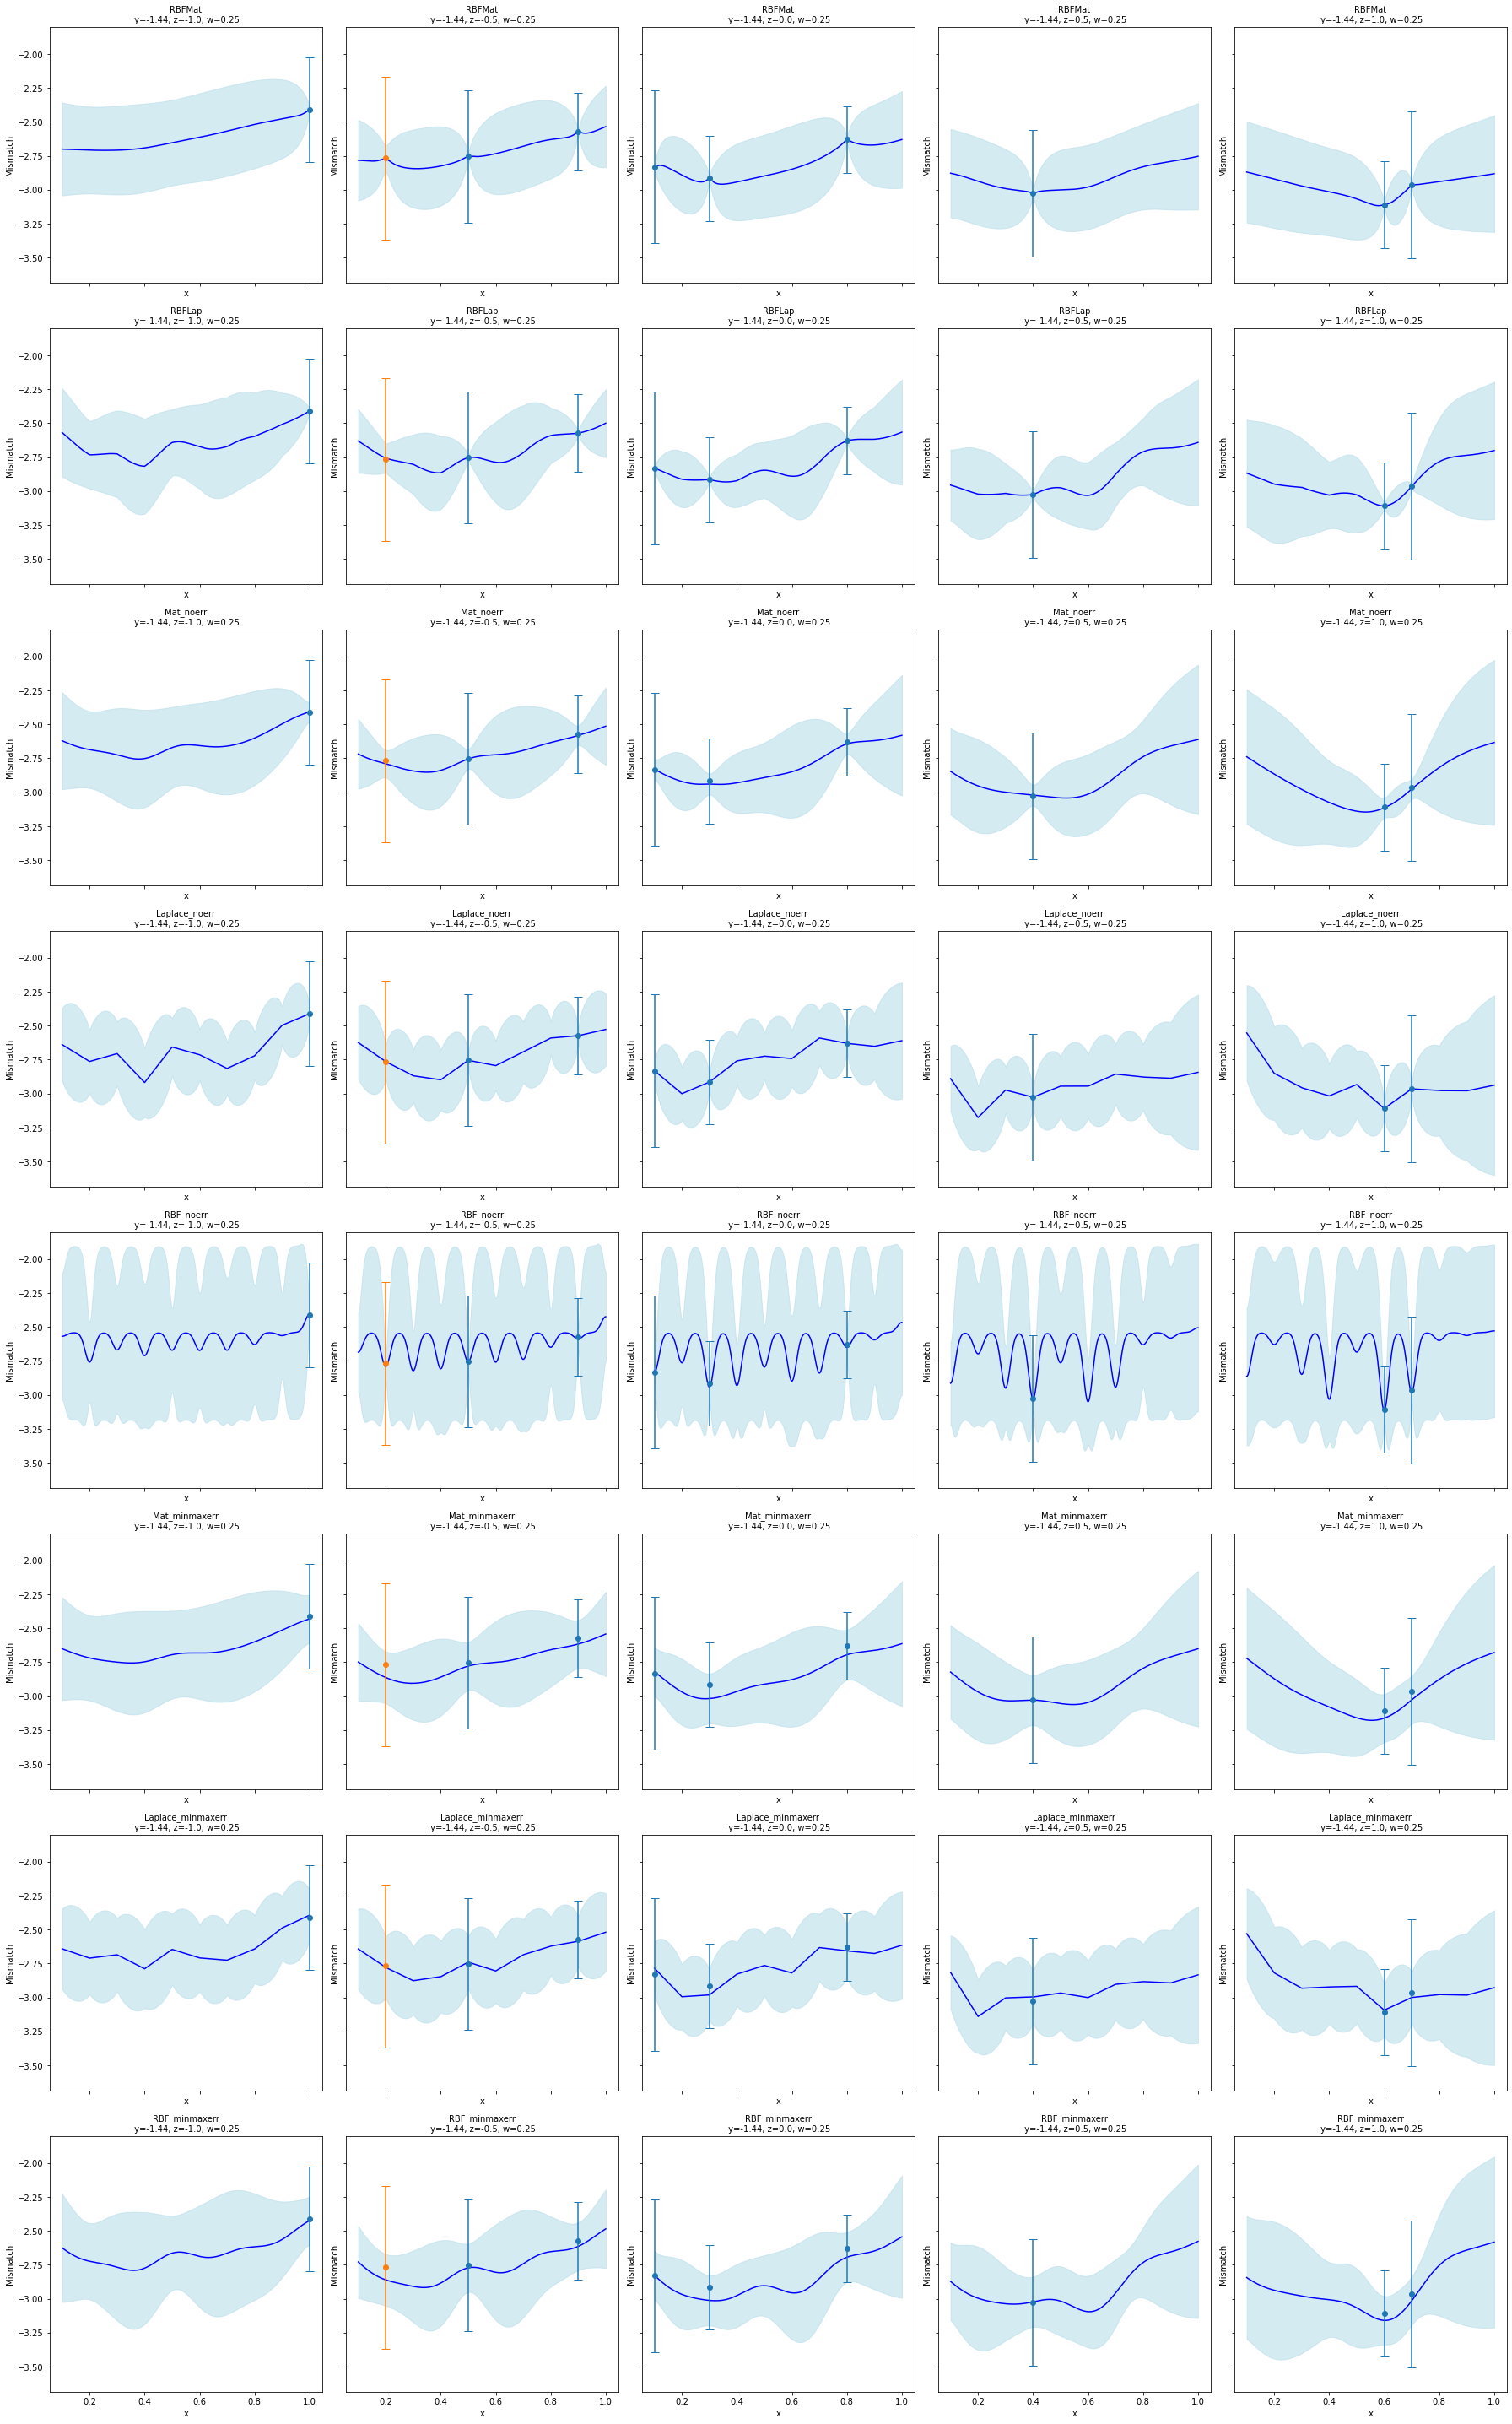
\includegraphics[width=0.8\textwidth]{LatexPlots/final_gps_plots/final_gps_ycuts.png}
    \caption{\todo{Improve caption} All 8 gps with cutting their y-axis}
    \label{fig:best8_ycuts}
\end{figure}


\begin{figure}[H]
    \centering
    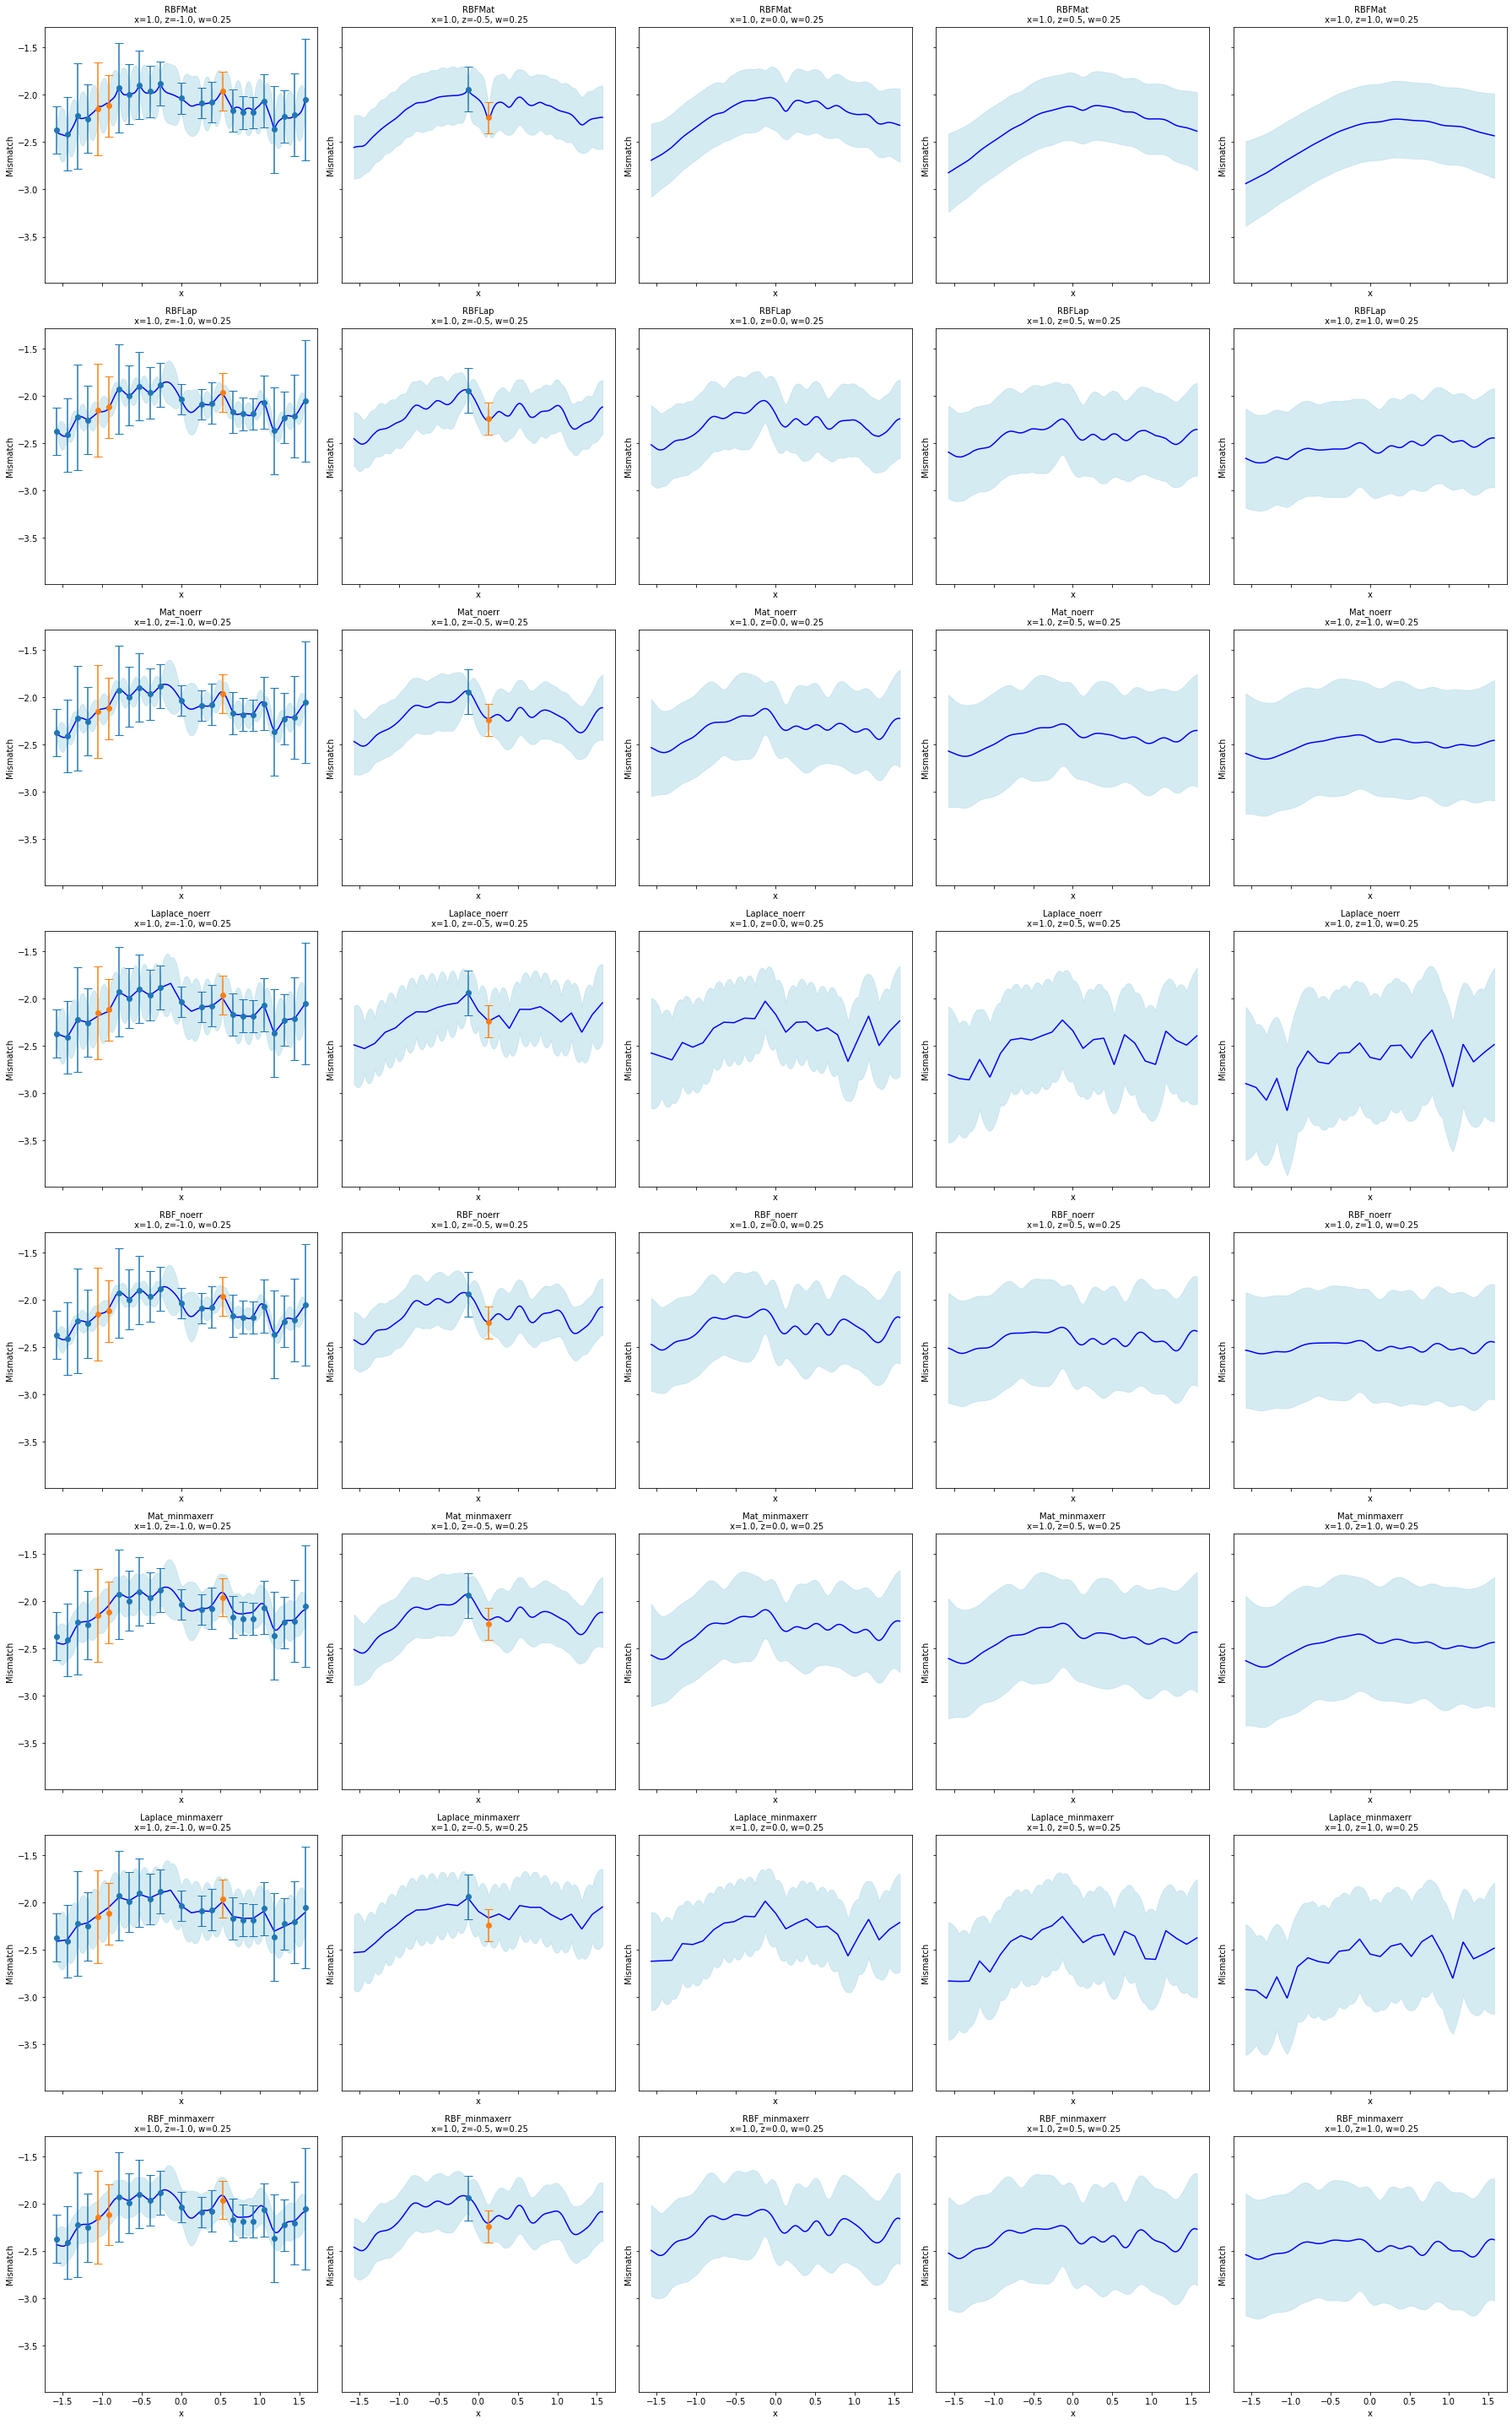
\includegraphics[width=0.8\textwidth]{LatexPlots/final_gps_plots/final_gps_xcuts.png}
    \caption{All 8 gps with cutting their x-axis}
    \label{fig:best8_xcuts}
\end{figure}

\begin{figure}[H]
    \centering
    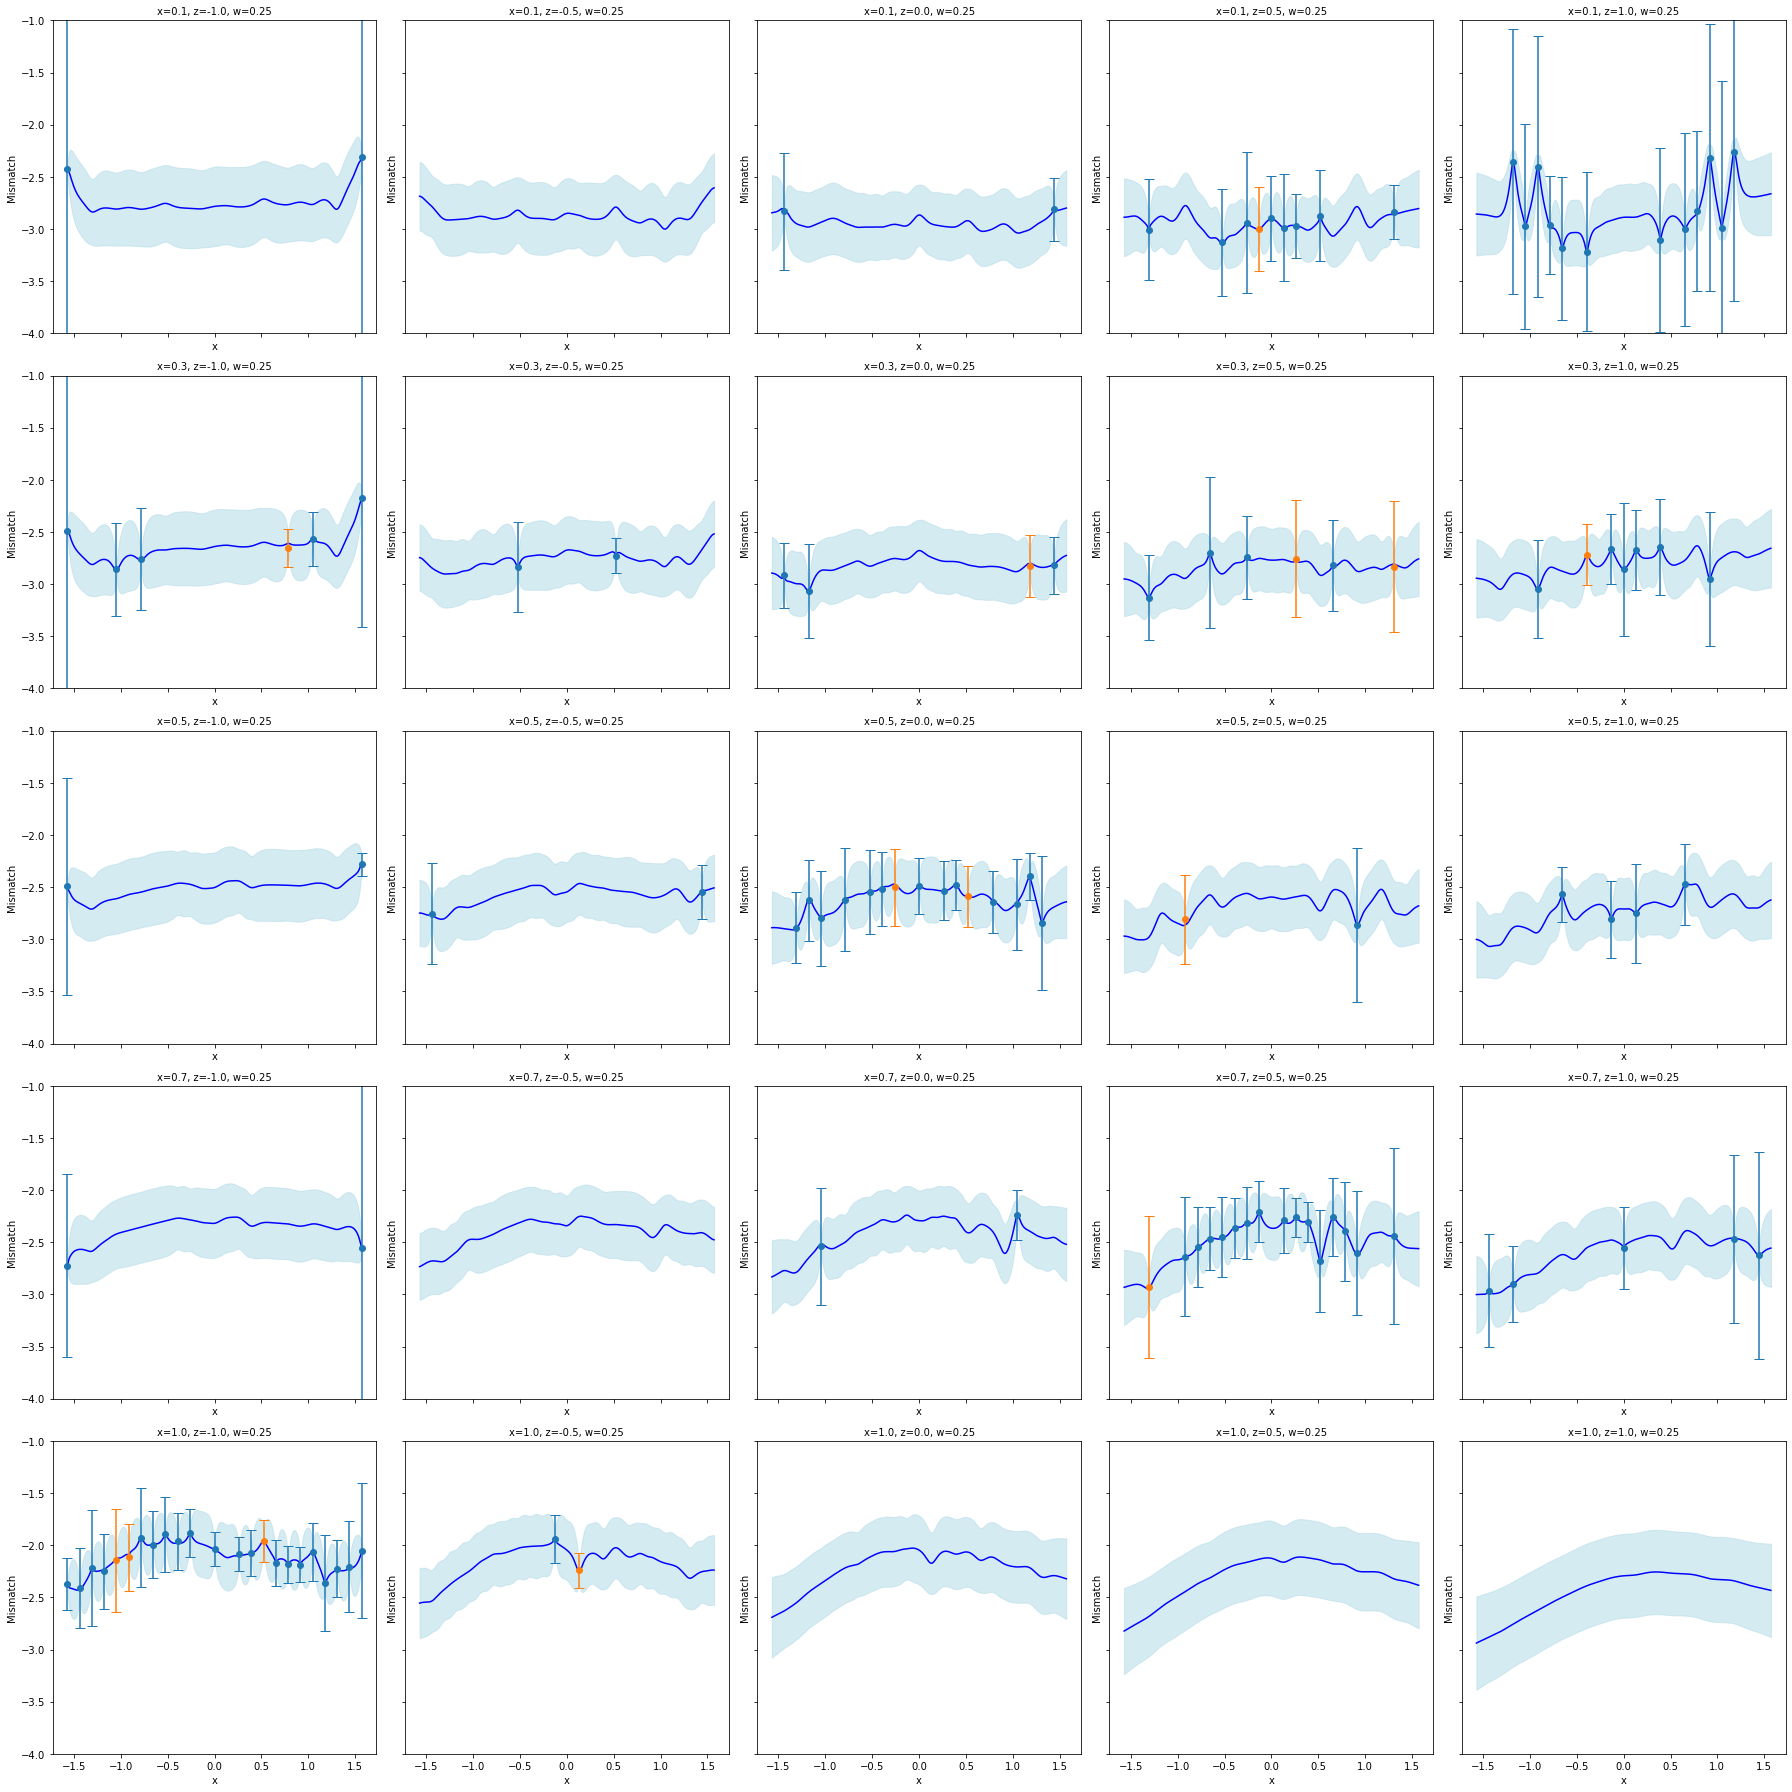
\includegraphics[width=0.8\textwidth]{LatexPlots/final_gps_plots/gps_rbfmatern_xcuts.png}
    \caption{Examining my chosen model RBF Matern kernel}
    \label{fig:RBF_Matern_xcuts}
\end{figure}


\subsection{Model Evaluation Table and graphs}
\label{appendix:D}

\begin{figure}[H]
    \centering
    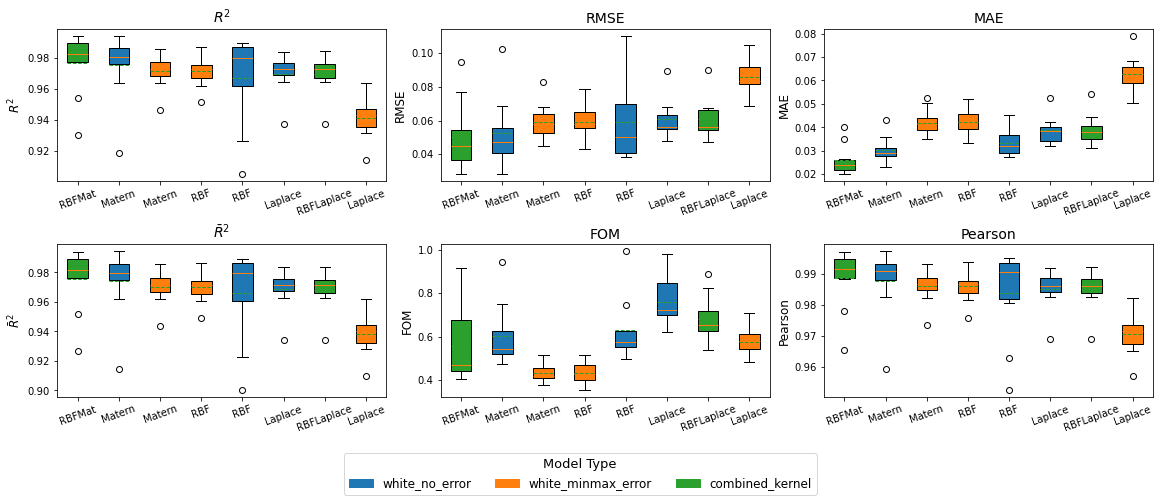
\includegraphics[width=0.8\textwidth]{LatexPlots/CV_plots/boxplots.png}
    \caption{Seeing how the best models performed over different clusters}
    \label{fig:boxplots}
\end{figure}

\begin{table}[H]
    \centering
    \caption{Final Model Rankings after training on 90\% and testing on 10\%}
    {\fontsize{7}{9.5}\selectfont
    \csvautotabular{LatexPlots/CV_plots/final_model_rankings.csv}}
    \label{tab:finalmadelsrankingtable}
\end{table}



\begin{table}[H]
    \centering
    \caption{All 32 Model Rankings from CV}
    {\fontsize{7}{9.5}\selectfont
    \csvautotabular{LatexPlots/CV_plots/model_rankings.csv}
    }
    \label{tab:rankingtable}
\end{table}
    

\subsection{Bin}
\label{appendix:bin}
\Sean{Moving Evaluation Metrics to Methods}

In figure \ref{tab:metrics-comparison}, we made a graphical representation of four out of six metrics used to evaluate our model’s accuracy. \cite{bible} discusses how these metrics provide a balanced assessment of model performance.
The Root Mean Squared Error (RMSE) and Mean Absolute Error (MAE) measure the average deviation of predictions from the true values, with RMSE penalizing larger errors more heavily.
The coefficient of determination \( R^2 \) quantifies how well the model predicts relative to the mean of the test set. It is computed as \( 1 \) minus the ratio of the squared residuals to the total variance. A value closer to \( 1 \) indicates better predictive performance.
The adjusted \( R^2 \) (\(\bar{R}^2\)) accounts for model complexity by penalizing excessive predictor variables, preventing overfitting.
The Figure of Merit (FOM) evaluates the ratio of a point’s prediction error to its associated standard deviation. A FOM near \( 1 \) is ideal, indicating that the model’s uncertainty estimates are well-calibrated. A FOM \( \ll 1 \) suggests an overly conservative model with large uncertainty, while a FOM \( \gg 1 \) may indicate overconfidence, failing to capture true variability.
The Pearson correlation coefficient measures the linear relationship between predictions and true values. A correlation of \( 1 \) (\(-1\)) signifies a perfect positive (negative) linear relationship, whereas a correlation of \( 0 \) indicates no linear association.



\begin{table}[H]
    \centering
    \renewcommand{\arraystretch}{4} % Adjust row spacing
    \setlength{\tabcolsep}{2pt} % Adjust column spacing
    \small % Reduce text size

    \begin{tabular}{|>{\centering\arraybackslash}m{2.5cm}|*{4}{>{\centering\arraybackslash}m{3cm}|}} 
        \hline
        \textbf{Metric Name} & \textbf{RMSE} & \textbf{\(R^2\)} & \textbf{FOM} & \textbf{Pearson Coefficient} \\ 
        \hline
        \textbf{Formula} & 
        \( \sqrt{\frac{1}{N} \sum (y_i - \hat{y}_i)^2} \)   & 
        \( 1 - \frac{\sum (y_i - \hat{y}_i)^2}{\sum (y_i - \bar{y})^2} \) &    
        \( \frac{RMSE}{\sigma} \) &  
        \( \frac{\text{cov}(y - \hat{y})}{\sigma_y \sigma_{\hat{y}}} \) \\ 
        \hline
        \textbf{Visual Illustration} &  
        \adjustbox{valign=c}{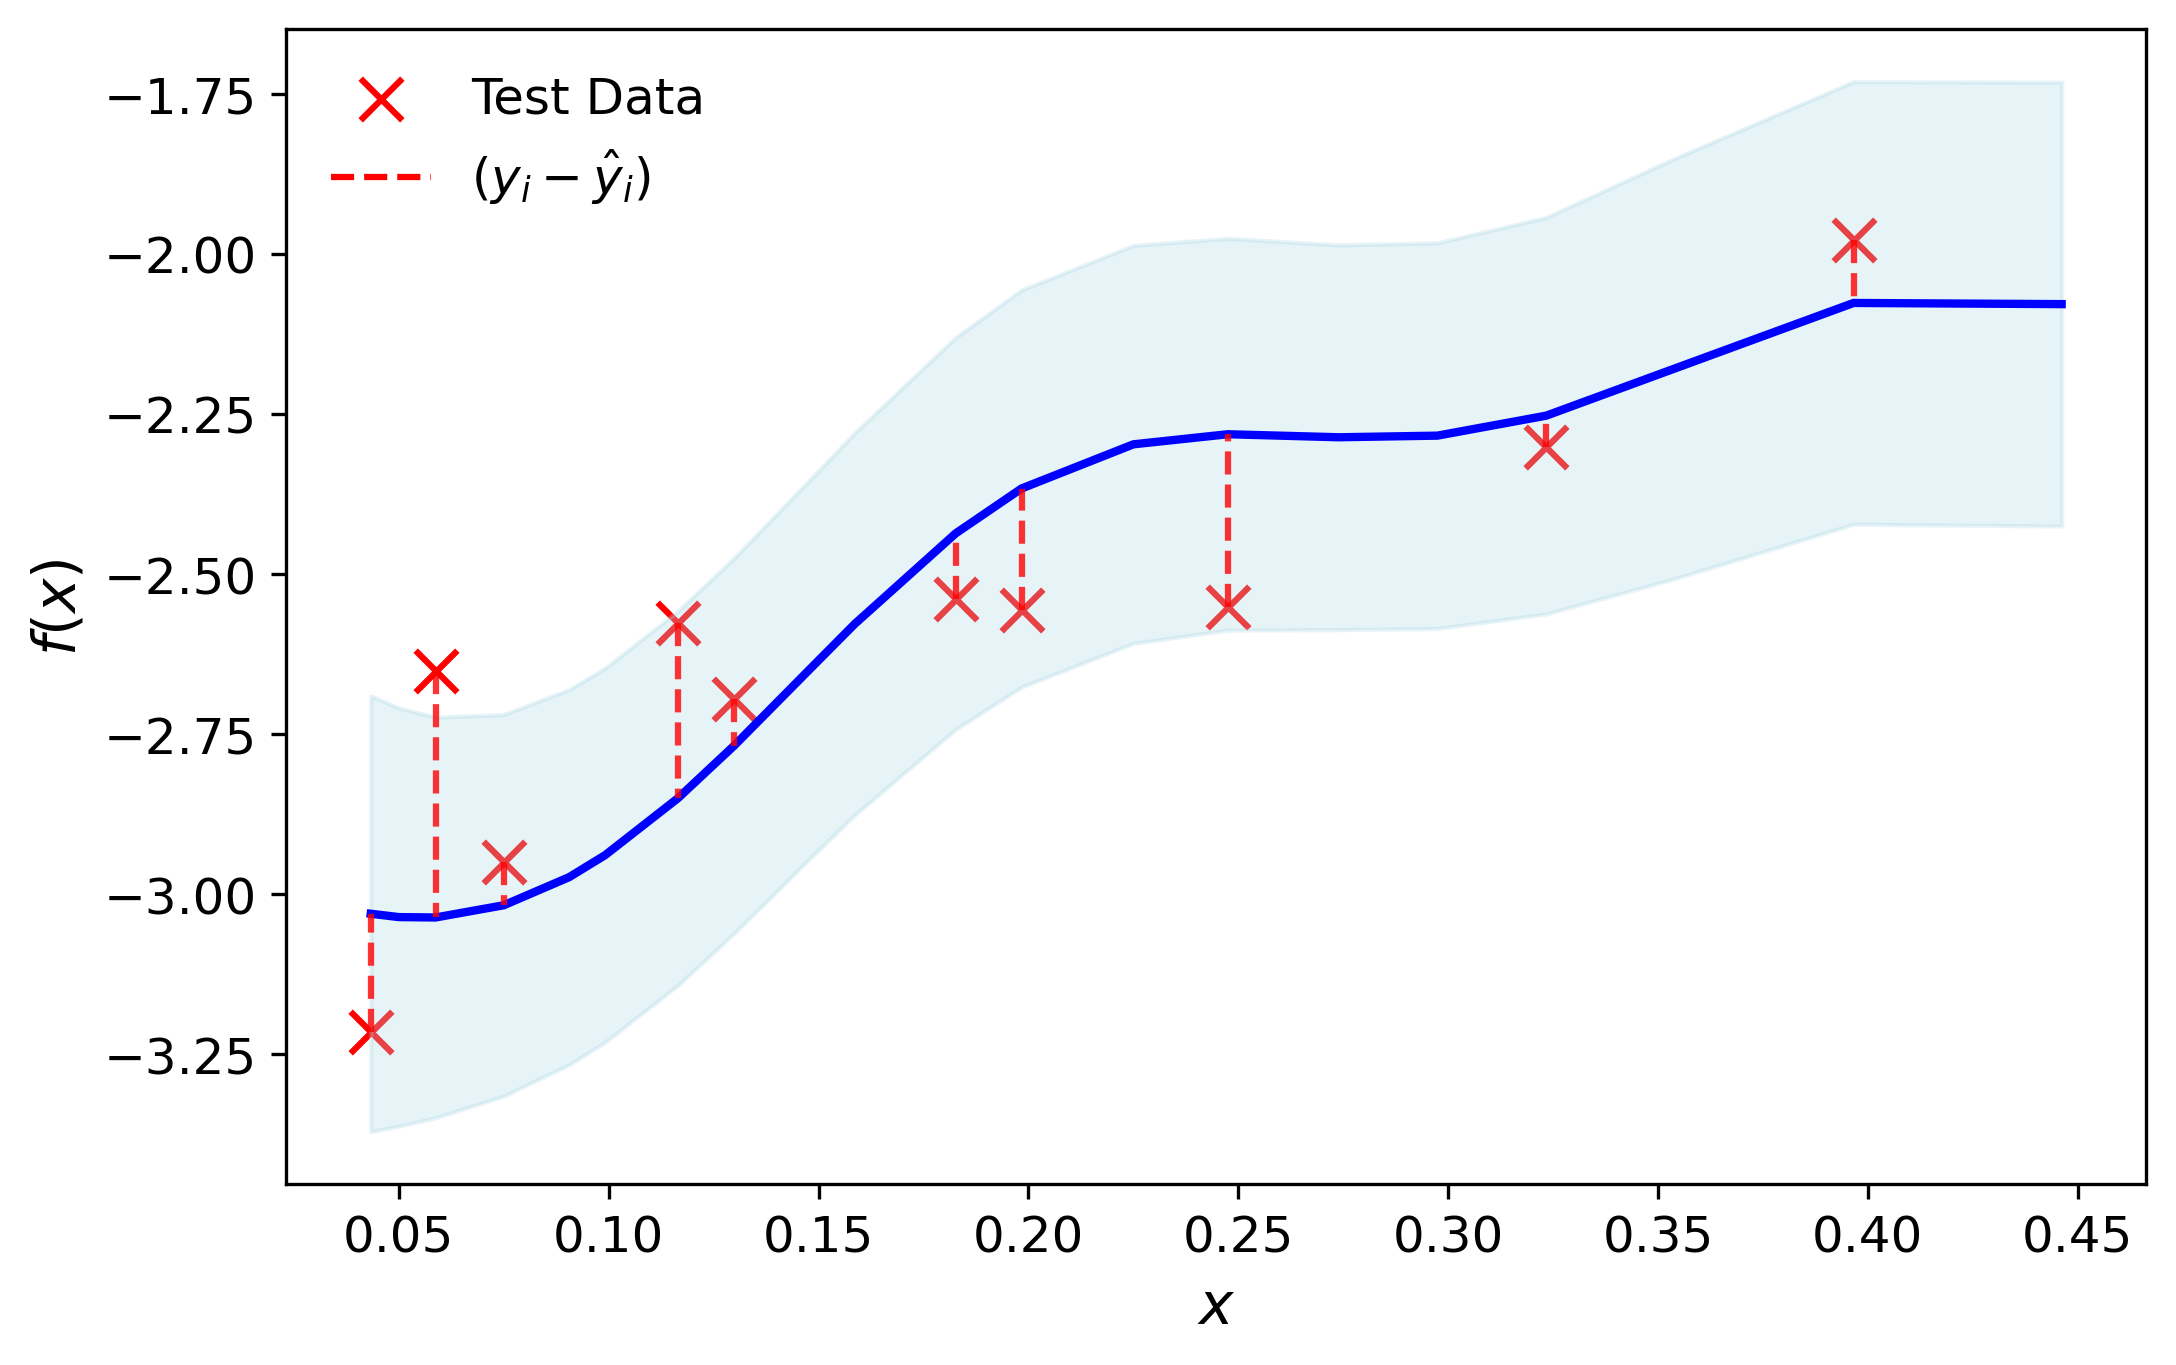
\includegraphics[width=3cm]{LatexPlots/1dplots/MAE.png}} &  
        \adjustbox{valign=c}{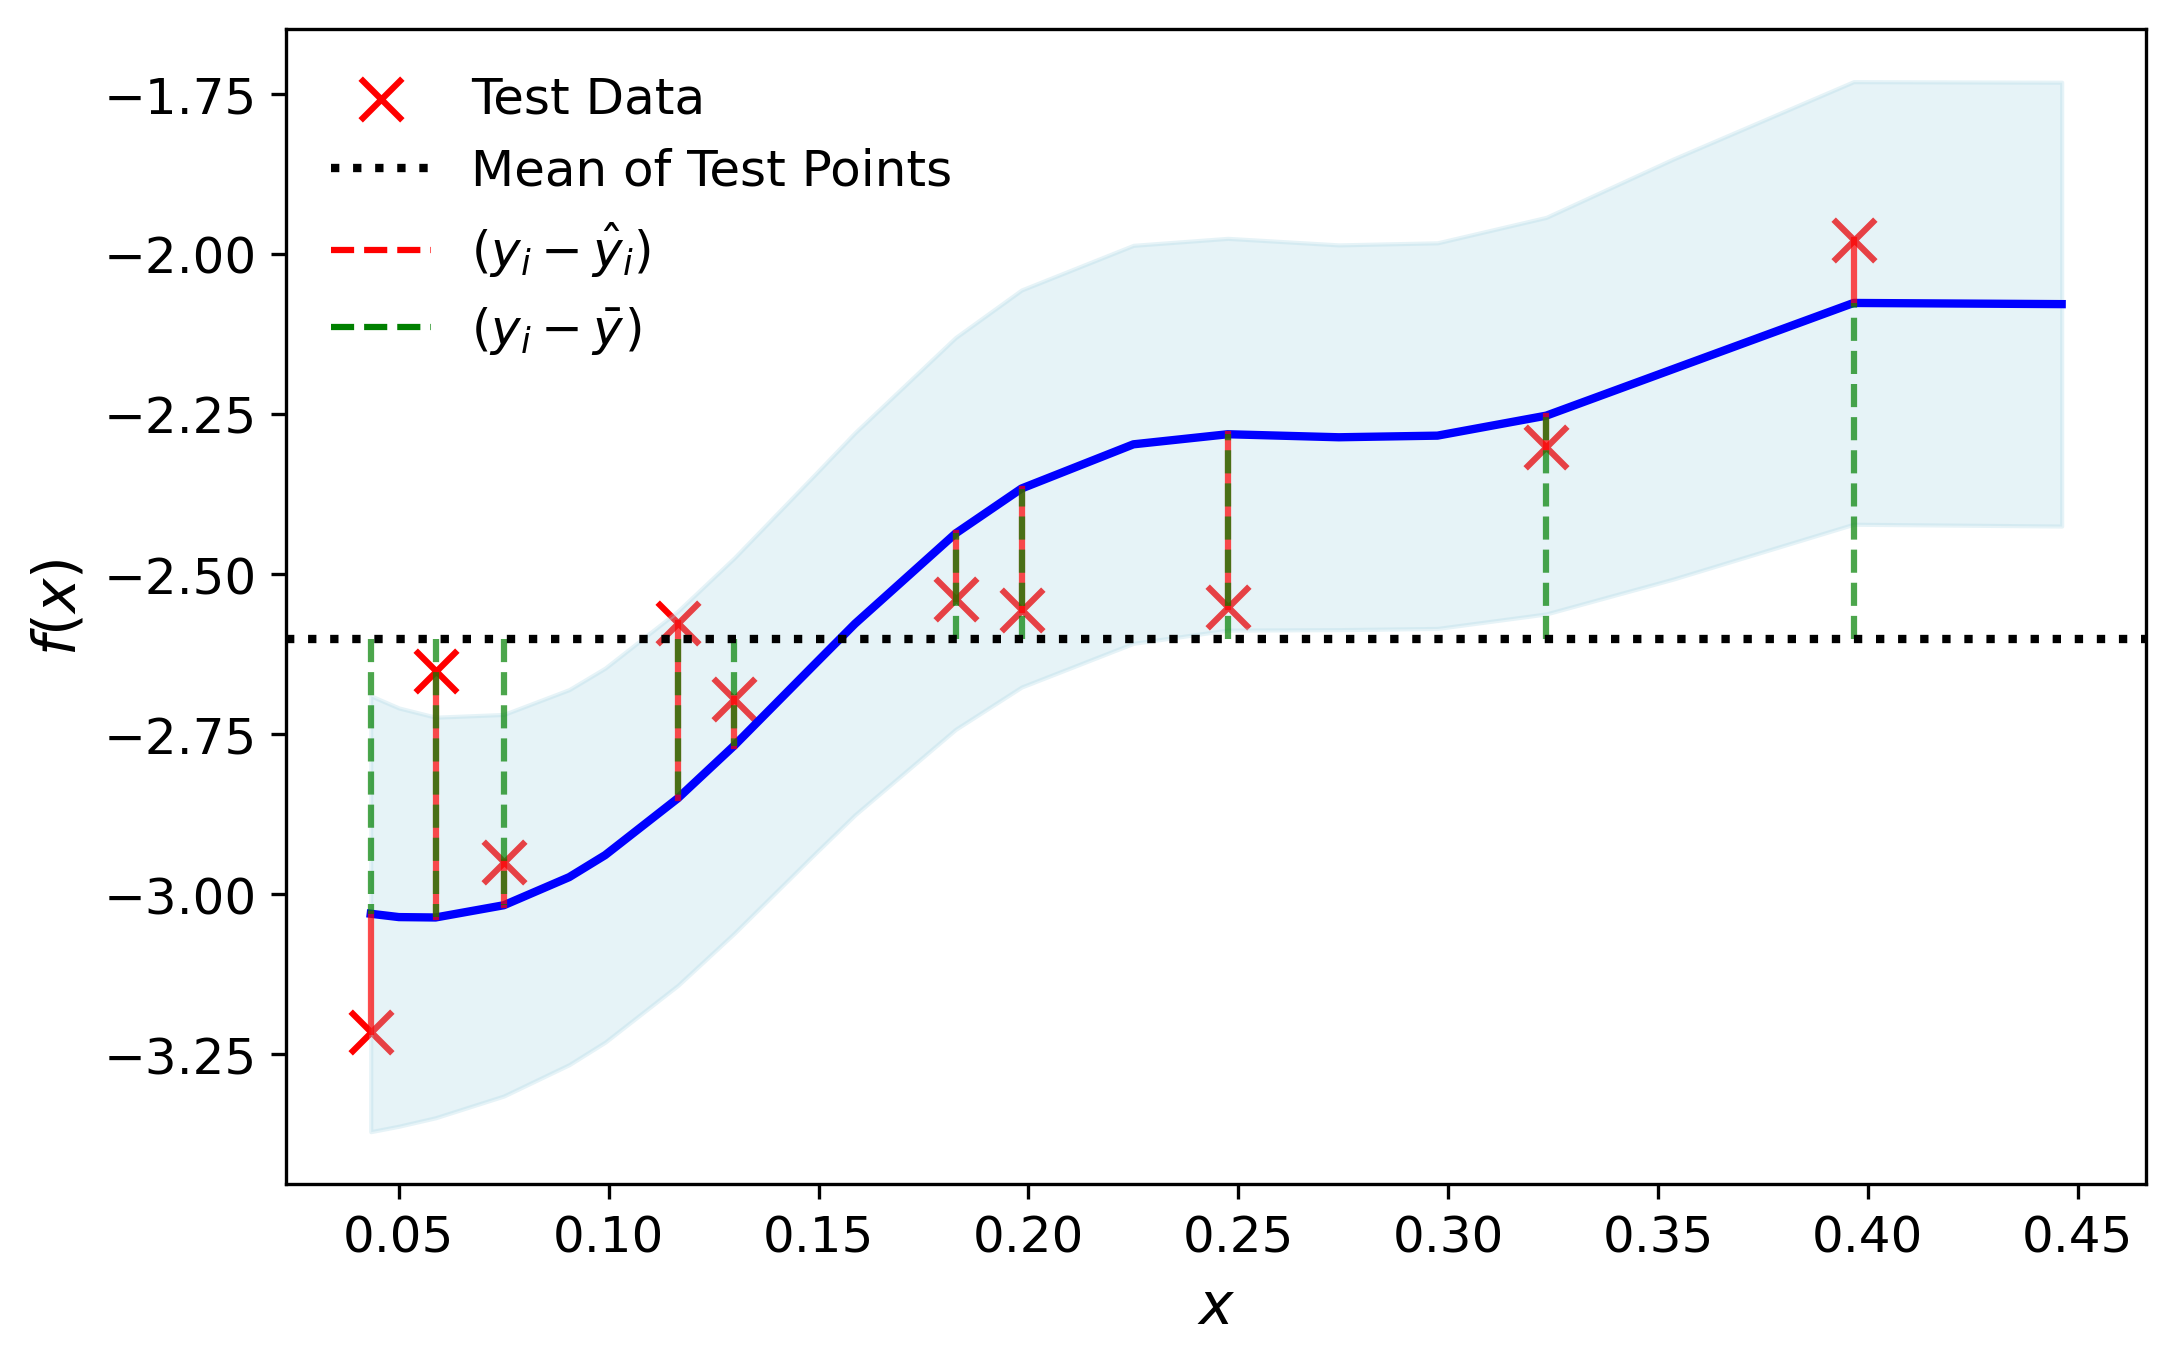
\includegraphics[width=3cm]{LatexPlots/1dplots/r2.png}} &  
        \adjustbox{valign=c}{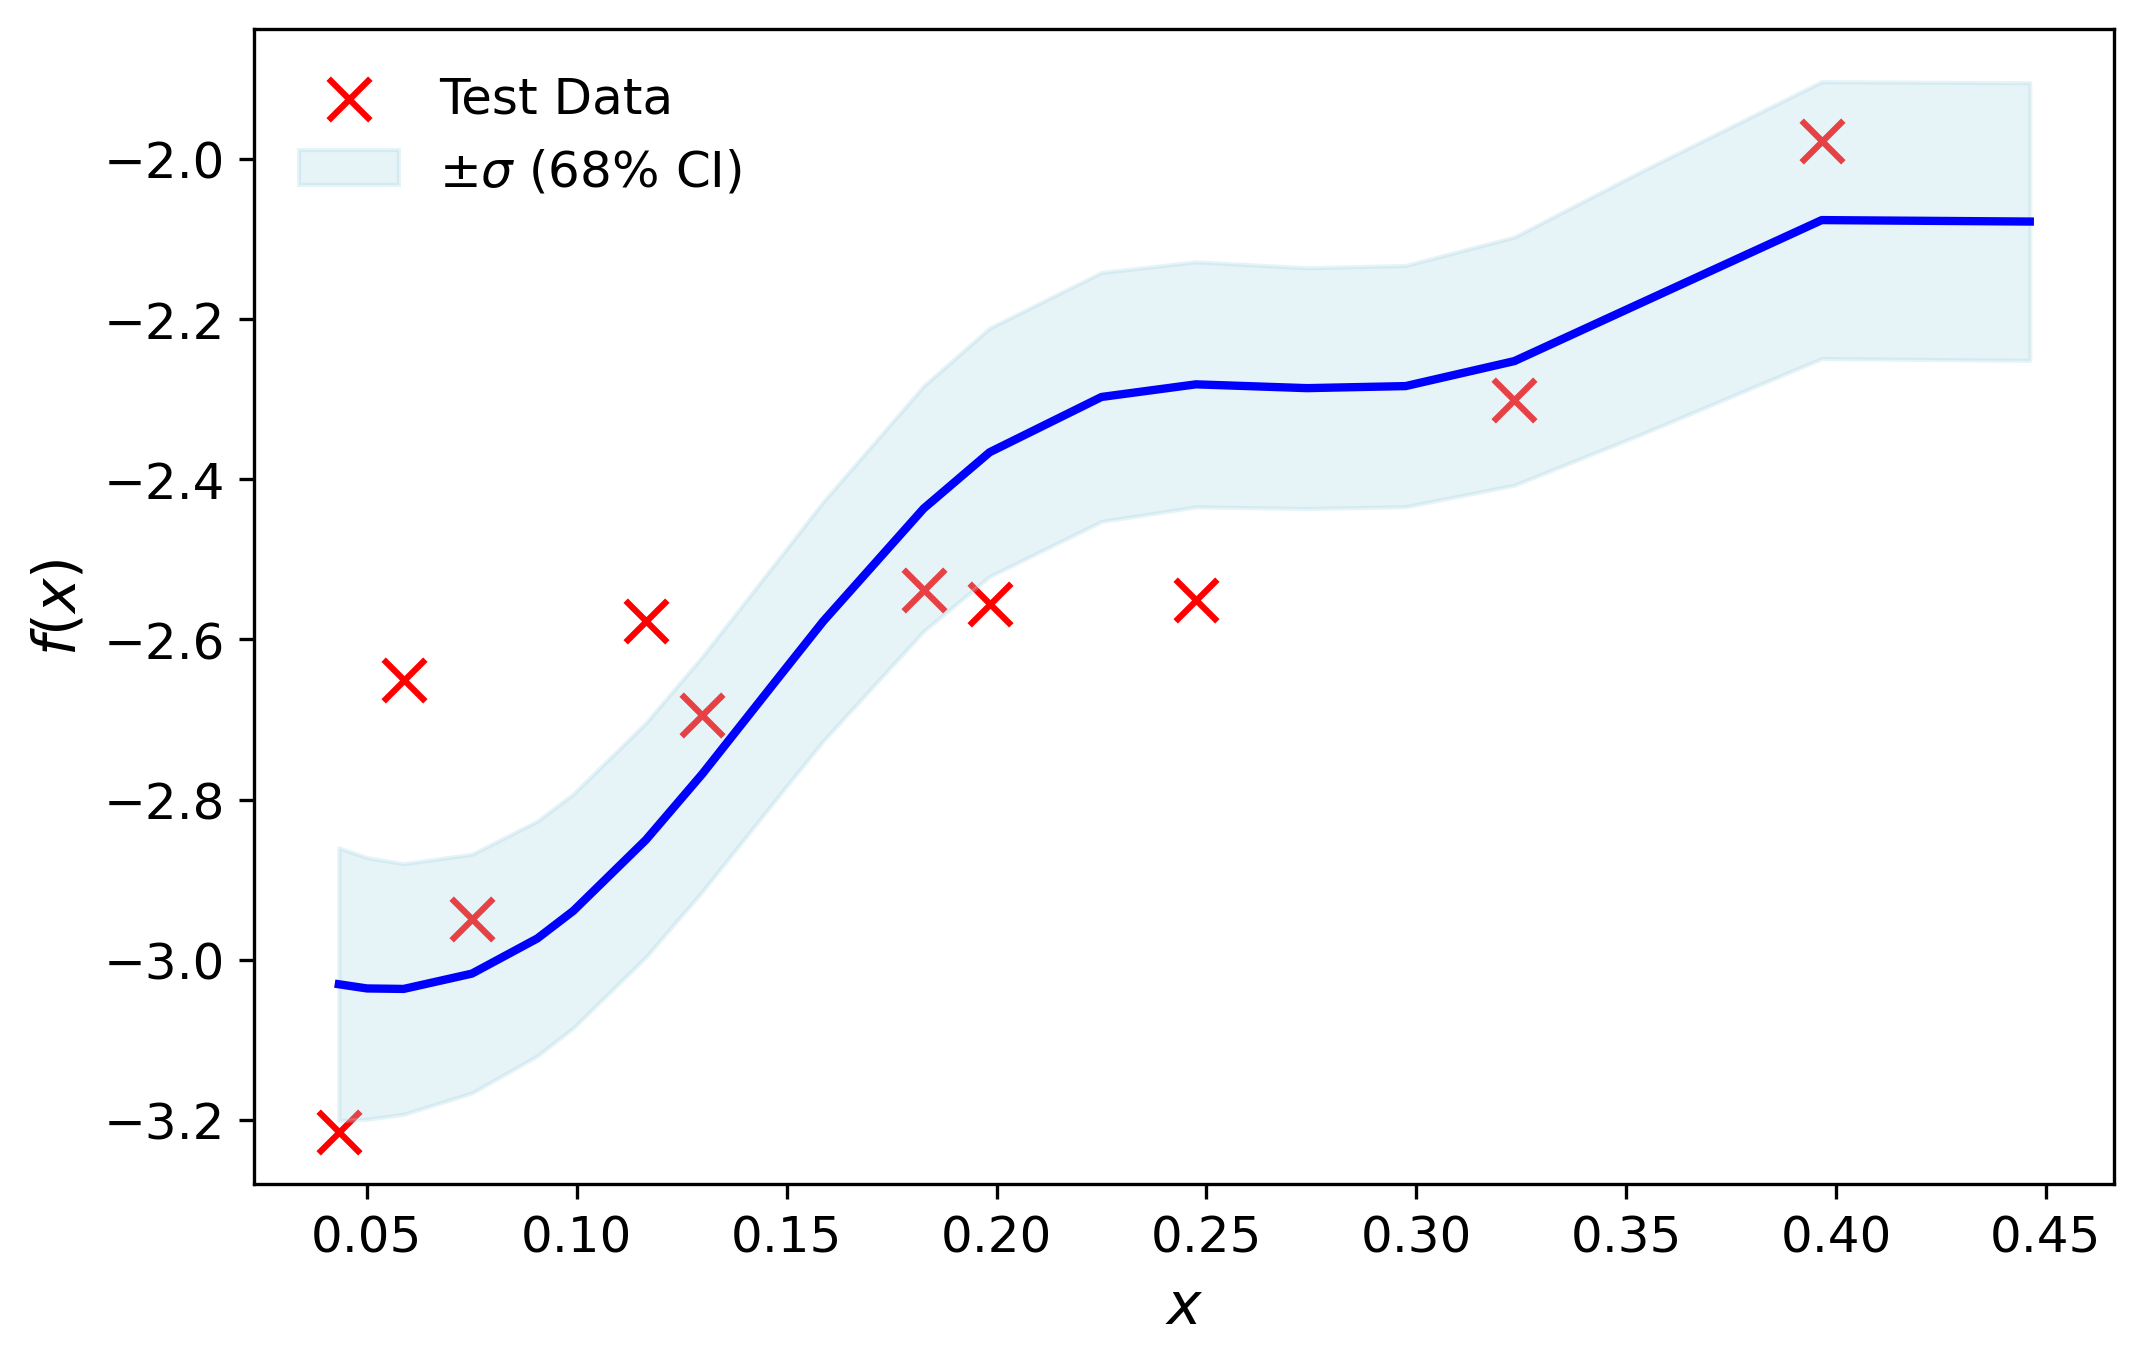
\includegraphics[width=3cm]{LatexPlots/1dplots/fom.png}} &  
        \adjustbox{valign=c}{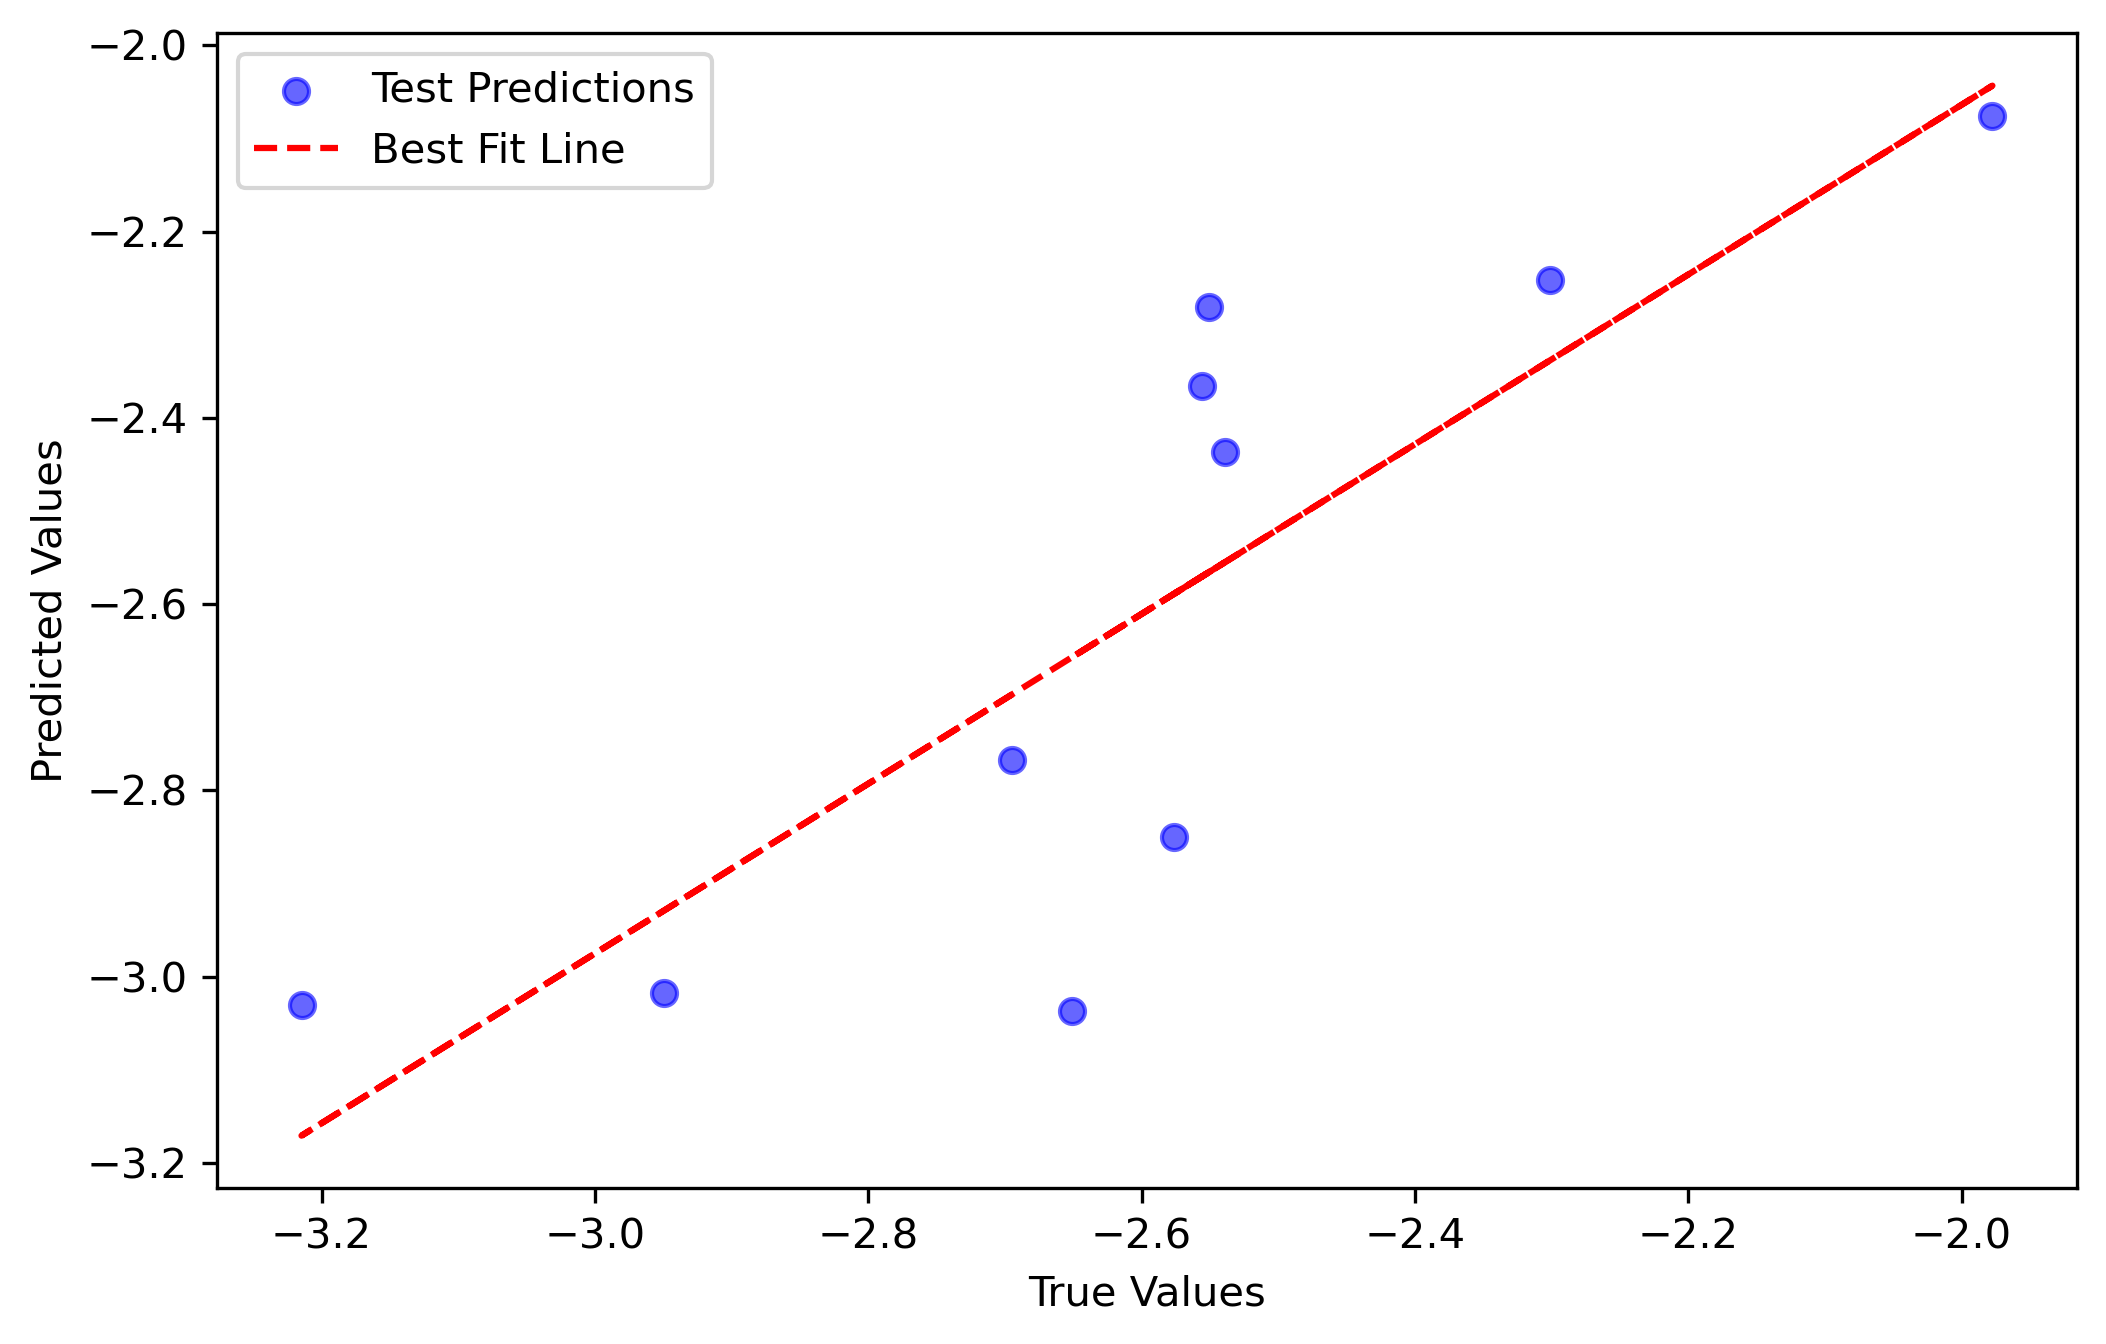
\includegraphics[width=3cm]{LatexPlots/1dplots/pearson.png}} \\  
        \hline
    \end{tabular}
    
    \caption{Comparison of different performance metrics used in evaluating models.  
    RMSE, \( R^2 \), FOM, and the Pearson Coefficient are included.  
    MAE is similar to RMSE but without squaring errors.  
    Adjusted \( R^2 \) accounts for the number of predictors and is slightly modified from \( R^2 \).
    The actual metrics for each graph are: RMSE = 0.2, \( R^2 \) = 0.6, FOM = 1.09, Pearson correlation = 0.8.}
    
    \label{tab:metrics-comparison}
\end{table}




\subsection{MCMC details}
\subsubsection*{Implementing MCMC}
\begin{figure}[H]
    \centering
    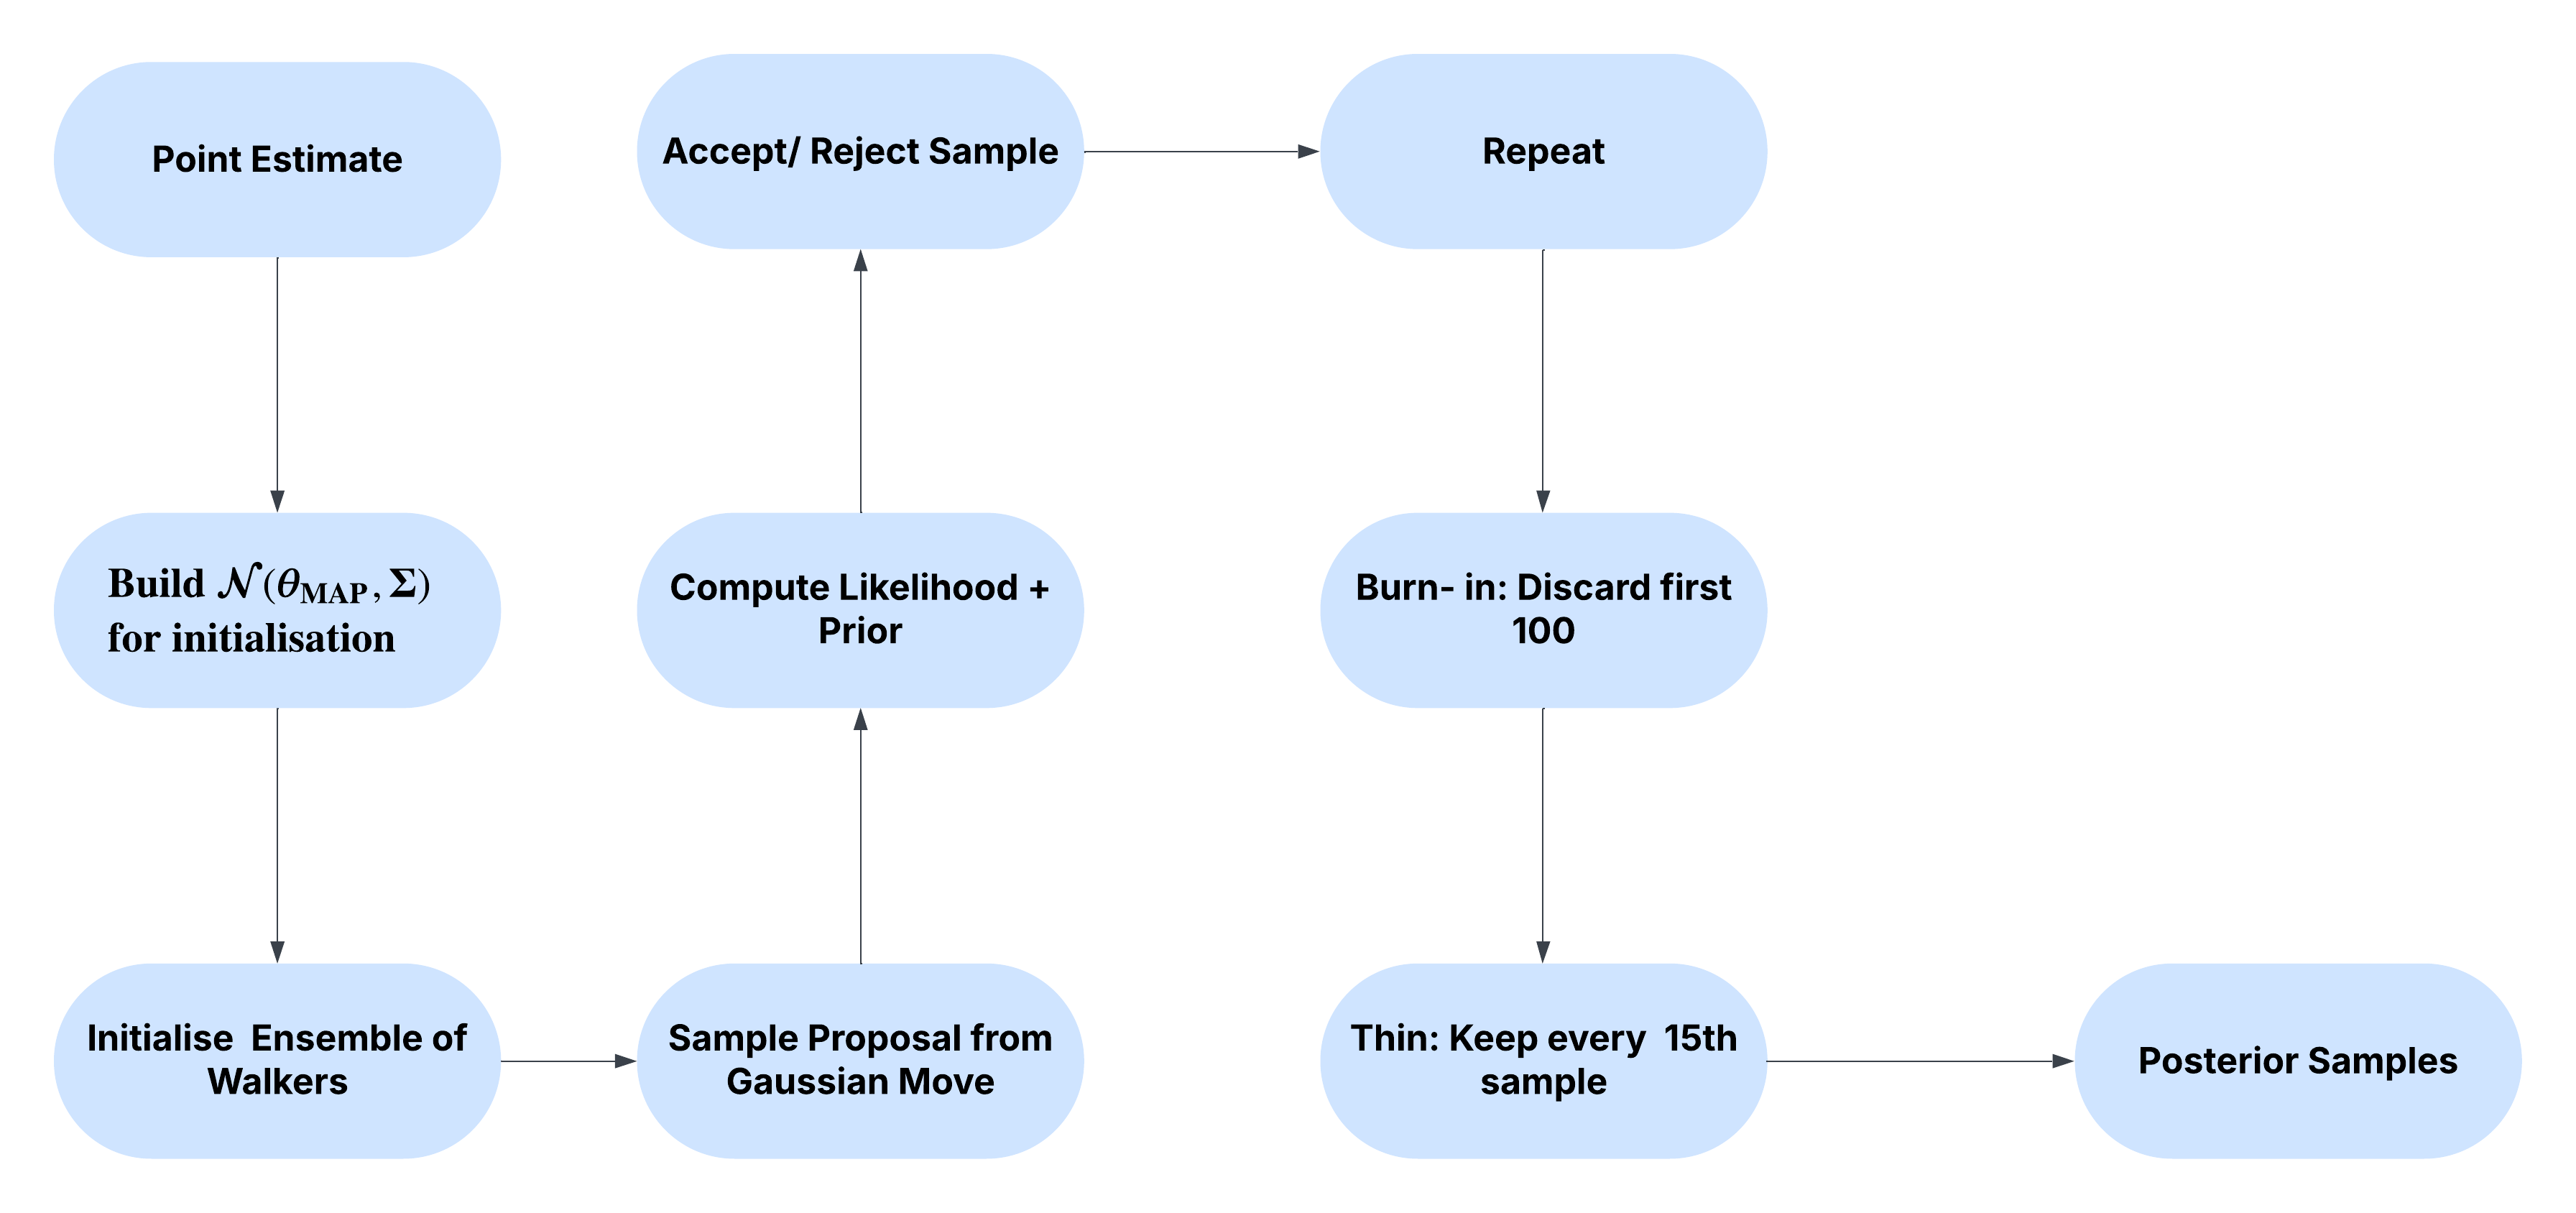
\includegraphics[width=0.8\textwidth]{LatexPlots/MCMC_Flow.png}
    \caption{Overview of the MCMC sampling procedure for Gaussian Process hyperparameter inference.
     This pipeline samples from the posterior \( p(\theta \mid \mathbf{y}, X) \) using a Metropolis-Hastings Gaussian proposal and an ensemble of walkers.}
    \label{fig:MCMC flowchart}
\end{figure}

\noindent
Before starting MCMC, we must decide which model we want to build the hyperparameter posterior for. This involves selecting one of the six kernels outlined in Section~\ref{sec: Kernels}, along with one of the three noise-modelling approaches described in Section~\ref{sec: Handlingnoise}. Once this model structure is fixed, we obtain initial point estimates for the hyperparameters by maximising the log marginal likelihood, as discussed in Section~\ref{sec: Hyper_parameters}.

\noindent
We then construct a multivariate normal distribution centred at this point estimate and sample from it to initialise each walker. From there, the walkers explore the hyperparameter space using a Gaussian proposal distribution with a specified covariance. At each step, we compute the sum of the log likelihood and log prior. The proposed sample is then accepted or rejected using the Metropolis-Hastings criterion \textcolor{red}{Could give more detail here}. This process is repeated for a fixed number of steps to generate a large set of samples.

\noindent
To ensure convergence and sample independence, we discard the first 100 samples from each walker as burn-in and apply a thinning factor of 15—retaining every 15\textsuperscript{th} sample. The resulting collection of samples forms our posterior distribution over hyperparameters, which we visualise using a kernel density estimate (KDE).


\subsection{Noise modeling using Monte Carlo Sampling}
\label{appendix:monte_carlo}

We assume the observation noise is Gaussian:
\[
\epsilon_i \sim \mathcal{N}(0, \sigma_i^2),
\]
we have the observed data \( y \) which is a noisy version of our true function values
\[
y = f + \epsilon, \quad \text{with } y \sim \mathcal{N}(f, \Sigma),
\]
where \( \Sigma = \mathrm{diag}(\sigma_1^2, \dots, \sigma_n^2) \).
Each true function value corresponds to our observed value \(\pm \epsilon\)
To account for this, we generate \( M \) noisy samples of the observations
\begin{equation}
    y^{(s)} = y + \epsilon^{(s)}, \quad \epsilon^{(s)} \sim \mathcal{N}(0, \Sigma).
\end{equation}
For each sampled dataset \( y^{(s)} \), we compute a GP posterior
\begin{equation}
    p(f_* \mid X, X_*, \theta, y^{(s)}).
\end{equation}
To obtain the final predictive distribution, we marginalize over these sampled posteriors:
\begin{equation}
    p(f_* \mid X, X_*, \theta, y) = \int p(f_* \mid X, X_*, \theta, y^{(s)}) \, p(y^{(s)} \mid y) \, dy^{(s)}.
\end{equation}
This integral is intractable so we approximate it using Monte Carlo integration where we get the average of each of our predictions on sampled datasets \(y^{(s)}\):
\begin{equation}
    p(f_* \mid X, X_*, \theta, y) \approx \frac{1}{M} \sum_{s=1}^{M} p(f_* \mid X, X_*, \theta, y^{(s)}).
\end{equation}

% %\printbibliography
% \bibliographystyle{acm}
% \bibliography{references}

\end{document}


